%%%%%%%%%%%%%%%%%%%%%%%%%%%%%%%%%%%%%%%%%
% Tufte-Style Book (Minimal Template)
% LaTeX Template
% Version 1.0 (5/1/13)
%
% This template has been downloaded from:
% http://www.LaTeXTemplates.com
%
% License:
% CC BY-NC-SA 3.0 (http://creativecommons.org/licenses/by-nc-sa/3.0/)
%
% IMPORTANT NOTE:
% In addition to running BibTeX to compile the reference list from the .bib
% file, you will need to run MakeIndex to compile the index at the end of the
% document.
%
%%%%%%%%%%%%%%%%%%%%%%%%%%%%%%%%%%%%%%%%%

%----------------------------------------------------------------------------------------
%	PACKAGES AND OTHER DOCUMENT CONFIGURATIONS
%----------------------------------------------------------------------------------------

\documentclass[a4paper,french,nobib,twoside,justified]{tufte-book} % Use the tufte-book class which in turn uses the tufte-common class
%\special{papersize=210mm,297mm}
\newcommand*\cleartoleftpage{%
  \clearpage
  \ifodd\value{page}\hbox{}\newpage\fi
}
%\usepackage{textcomp}
\hypersetup{colorlinks} % Comment this line if you don't wish to have colored links
\usepackage{microtype} % Improves character and word spacing

\usepackage{booktabs} % Better horizontal rules in tables
\usepackage{graphicx} % Needed to insert images into the document
\graphicspath{{graphics/}} % Sets the default location of pictures
%\setkeys{Gin}{width=\linewidth,totalheight=\textheight,keepaspectratio} % Improves figure scaling

\usepackage{fancyvrb} % Allows customization of verbatim environments
\fvset{fontsize=\normalsize} % The font size of all verbatim text can be changed here

% this is a local hack, to get the fancy UBdx page
\usepackage{first-page}

\usepackage{makeidx} % Used to generate the index
\makeindex % Generate the index which is printed at the end of the document

\usepackage[utf8]{inputenc}
\usepackage{listings,lstautogobble}
%\usepackage{luatextra}
\usepackage{mymacros}
%\usepackage{fontspec}
%\usepackage{polyglossia}
\usepackage{babel}
\usepackage{multirow}
\usepackage{amssymb}
\usepackage{amsmath}
\usepackage{dsfont}
\usepackage{mathrsfs}
\usepackage[normalem]{ulem} 
\usepackage{alltt}
\usepackage{stmaryrd} % for \llbracket ⟦ in math mode
\usepackage{MnSymbol} % for \llangle << in math mode
\usepackage{color, colortbl}
%\usepackage{enumerate}
\usepackage{tikz}
\usetikzlibrary{shapes.geometric, arrows,automata,positioning}

%\usepackage[rounded]{syntax}

% \usepackage{lscape}
% \usepackage{caption}
% \usepackage{float}
% \usepackage{pdfpages}


% \usepackage{subfigure}
% \usepackage{calc}
% \usepackage{amstext}
% \usepackage{amsthm}
% \usepackage{multicol}
% \usepackage{pslatex}

% \usepackage{multicol}

%\usepackage{cite}
%\usepackage[headheight=25pt]{geometry}


% make figure numbering be linear in the document, not per-chapter.
\usepackage{chngcntr}
\counterwithout{figure}{chapter}
%\counterwithout{listing}{chapter}
% make table numbering be linear in the document, not per-chapter.
\counterwithout{table}{chapter}

%\usepackage{calc}
%%%%%%%%%%%%%%%%%%%%%%%%%%%%%%%%%%%%%%%%%%%%%%%%%%%%%%%%%%%
%%% holes: stolen from Literate Agda paper.
%Define a reference depth. 
%You can choose either relative or absolute.
%--------------------------
\newlength{\DepthReference}
\settodepth{\DepthReference}{g}%relative to a depth of a letter.
%\setlength{\DepthReference}{6pt}%absolute value.

%Define a reference Height. 
%You can choose either relative or absolute.
%--------------------------
\newlength{\HeightReference}
\settoheight{\HeightReference}{T}
%\setlength{\HeightReference}{6pt}

%--------------------------
\newlength{\Width}%

\newcommand{\MyColorBox}[2][red]%
{%
    \settowidth{\Width}{#2}%
    %\setlength{\fboxsep}{0pt}%
    \colorbox{#1}%
    {%      
        \raisebox{-\DepthReference}%
        {%
                \parbox[b][\HeightReference+\DepthReference][c]{\Width}{\centering#2}%
        }%
    }%
}
\colorlet{Hole}{Dandelion!25!white}

% the hole-in-term symbol for Chapter 3
% \newcommand{\hole}{\ensuremath{\quad\cdot\quad}}
\newcommand{\minihole}{\MyColorBox[Hole]{\ensuremath{\{\,\,\}_{?}}}{}}
\newcommand{\hole}{\ensuremath{\quad}\minihole\ensuremath{\quad}}
%%%%%%%%%%%%%%%%%%%%%%%%%%%%%%%%%%%%%%%%%%%%%%%%%%%%%%%%%%%


%%% Local Variables:
%%% mode: latex
%%% TeX-master: t
%%% End:


%% Tweaking PDF bookmarks
\usepackage[numbered]{bookmark}
\hypersetup{%
  bookmarksdepth=3%
}

% "0" would disable section numbering, should i want that... Tufte
% doesn't like numbers.
\setcounter{secnumdepth}{1}
\setcounter{tocdepth}{1}

% have the bib neatly positioned after the rest of the ToC items
\newlength{\beforebibskip}
\setlength{\beforebibskip}{0em} % this might need to become 1em or other
%\selectlanguage{french}

\usepackage{hyphenat}
% more float registers
%\usepackage{etex}
%\reserveinserts{30}

\usepackage[
backend = biber,
citereset=none,
%style = debug,
style = authoryear,
dateabbrev = false,
% dashed = false, % repeat full author names every occurrence
maxbibnames = 99, % don't use 'et al.' in the Bibliography
maxcitenames=2,
citestyle = authoryear,
language = british
]{biblatex}
\addbibresource{bibliography.bib} 
% DONE really use biblatex, not the citation hack here
% https://tex.stackexchange.com/questions/45934/can-i-use-biblatex-with-tufte-classes
\DeclareBibliographyCategory{fullcited}

\newcommand{\mybibexclude}[1]{\addtocategory{fullcited}{#1}}

\DeclareNameAlias{sortname}{first-last} % this makes the names as
                                        % displayed in the
                                        % Bibliography consistent, in
                                        % my case not Last, First
                                        % followed by First Last,
                                        % First Last, ...
\usepackage{booktabs}
\usepackage{bbding} % for \Checkmark and \XSolidBrush

%\usepackage{calc}
%%%%%%%%%%%%%%%%%%%%%%%%%%%%%%%%%%%%%%%%%%%%%%%%%%%%%%%%%%%
%%% holes: stolen from Literate Agda paper.
%Define a reference depth. 
%You can choose either relative or absolute.
%--------------------------
\newlength{\DepthReference}
\settodepth{\DepthReference}{g}%relative to a depth of a letter.
%\setlength{\DepthReference}{6pt}%absolute value.

%Define a reference Height. 
%You can choose either relative or absolute.
%--------------------------
\newlength{\HeightReference}
\settoheight{\HeightReference}{T}
%\setlength{\HeightReference}{6pt}

%--------------------------
\newlength{\Width}%

\newcommand{\MyColorBox}[2][red]%
{%
    \settowidth{\Width}{#2}%
    %\setlength{\fboxsep}{0pt}%
    \colorbox{#1}%
    {%      
        \raisebox{-\DepthReference}%
        {%
                \parbox[b][\HeightReference+\DepthReference][c]{\Width}{\centering#2}%
        }%
    }%
}
\colorlet{Hole}{Dandelion!25!white}

% the hole-in-term symbol for Chapter 3
% \newcommand{\hole}{\ensuremath{\quad\cdot\quad}}
\newcommand{\minihole}{\MyColorBox[Hole]{\ensuremath{\{\,\,\}_{?}}}{}}
\newcommand{\hole}{\ensuremath{\quad}\minihole\ensuremath{\quad}}
%%%%%%%%%%%%%%%%%%%%%%%%%%%%%%%%%%%%%%%%%%%%%%%%%%%%%%%%%%%


%%% Local Variables:
%%% mode: latex
%%% TeX-master: t
%%% End:


\makeatletter
% We'll keep track of the old/seen bibkeys in this list.
\def\@tufte@old@bibkeys{}

% prevent url, doi, isbn, issn from appearing in margin-citations.
\AtEveryCite{%
 \DeclareFieldFormat{url}{}%
 \DeclareFieldFormat{urldate}{}%
 \DeclareFieldFormat{doi}{}%
 \DeclareFieldFormat{isbn}{}%
 \DeclareFieldFormat{issn}{}%
}%


% This macro prints the full citation if it's the first time it's been used
% and a shorter citation if it's been used before.
\newcommand{\@tufte@print@margin@citation}[1]{%
  % print full citation if bibkey is not in the old bibkeys list
  \xifinlist{#1}{\@tufte@old@bibkeys}{%
    \cite{#1}% print short entry
  }{%
    \fullcite{#1}\unskip% print full entry
    % add bibkey to the old bibkeys list
    \listxadd{\@tufte@old@bibkeys}{#1}%
  }%
}%

% We've modified this Tufte-LaTeX macro to call \@tufte@print@margin@citation
% instead of \bibentry.
\renewcommand{\@tufte@normal@cite}[2][0pt]{%
  % Empty variable for last bibkey, 
  \let\@temp@last@bibkey\@empty%
  % Snag the last bibentry in the list for later comparison
  \@for\@temp@bibkey:=#2\do{\let\@temp@last@bibkey\@temp@bibkey}%
  \sidenote[][#1]{%
    % Loop through all the bibentries, separating them with semicolons and spaces
    \normalsize\normalfont\@tufte@citation@font%
    \setcounter{@tufte@num@bibkeys}{0}%
    \@for\@temp@bibkeyx:=#2\do{%
      % Check if we're already dealing with the last key in the list of to-cite keys.
      \ifthenelse{\equal{\@temp@last@bibkey}{\@temp@bibkeyx}}{%
        % Add "and " to the last one. E.g. a; b; c; and d.
        % unless there was only 1 (checked with num@bibkeys).
        \ifthenelse{\equal{\value{@tufte@num@bibkeys}}{0}}{}{and\ }%
        \@tufte@trim@spaces\@temp@bibkeyx% trim spaces around bibkey
        \@tufte@print@margin@citation{\@temp@bibkeyx}%
      }{%
        \@tufte@trim@spaces\@temp@bibkeyx% trim spaces around bibkey
        \@tufte@print@margin@citation{\@temp@bibkeyx};\space%
      }%
      \stepcounter{@tufte@num@bibkeys}%
    }%
  }%
}%

\newcommand{\@tufte@normal@cite@separate}[2][0pt]{%
  \@for\@temp@bibkeyx:=#2\do{%
    \sidenote[][#1]{%
      % Loop through all the bibentries, separating them with semicolons and spaces
      \normalsize\normalfont\@tufte@citation@font%
      \@tufte@trim@spaces\@temp@bibkeyx% trim spaces around bibkey
      \@tufte@print@margin@citation{\@temp@bibkeyx}%
    }%
  }%
}%

%\renewcommand{\cite}[2][0pt]{\sidenote[][#1]{\fullcite{#2}}}% for biber / biblatex
\newcommand{\paulciteseparate}[2][0pt]{\@tufte@normal@cite@separate[#1]{#2}}% 
%\newcommand{\paulcite}[2][0pt]{\sidenote[][#1]{\fullcite{#2}}}% 
\newcommand{\paulcite}[2][0pt]{\@tufte@normal@cite[#1]{#2}}% 

% Calling this macro will reset the list of remembered citations. This is
% useful if you want to revert to full citations at the beginning of each
% chapter.
\newcommand{\resetcitations}{%
  \gdef\@tufte@old@bibkeys{}%
}
\makeatother

%%% Local Variables:
%%% mode: latex
%%% TeX-master: "paul-thesis"
%%% End:


\newcommand{\hangp}[1]{\makebox[0pt][r]{(}#1\makebox[0pt][l]{)}} % New command to create parentheses around text in tables which take up no horizontal space - this improves column spacing
\newcommand{\hangstar}{\makebox[0pt][l]{*}} % New command to create asterisks in tables which take up no horizontal space - this improves column spacing

\usepackage{xspace} % Used for printing a trailing space better than using a tilde (~) using the \xspace command

\newcommand{\monthyear}{\ifcase\month\or January\or February\or March\or April\or May\or June\or July\or August\or September\or October\or November\or December\fi\space\number\year} % A command to print the current month and year

% \newcommand{\openepigraph}[2]{ % This block sets up a command for printing an epigraph with 2 arguments - the quote and the author
% \begin{fullwidth}
% \sffamily\large
% \begin{doublespace}
% \noindent\allcaps{#1}\\ % The quote
% \noindent\allcaps{#2} % The author
% \end{doublespace}
% \end{fullwidth}
% }

%\newcommand{\blankpage}{\newpage\hbox{}\thispagestyle{empty}\newpage} % Command to insert a blank page

%----------------------------------------------------------------------------------------
%	BOOK META-INFORMATION
%----------------------------------------------------------------------------------------

% \title{Une approche événementielle pour le développement de services multi-métiers dédiés à l'assistance domiciliaire}
% %\subtitle{}
% \author{Adrien Carteron}
% \date{22 décembre 2017}

%----------------------------------------------------------------------------------------

\makeatletter

\newrobustcmd*{\parentexttrack}[1]{%
  \begingroup
  \blx@blxinit
  \blx@setsfcodes
  \blx@bibopenparen#1\blx@bibcloseparen
  \endgroup}

\AtEveryCite{%
  \let\parentext=\parentexttrack%
  \let\bibopenparen=\bibopenbracket%
  \let\bibcloseparen=\bibclosebracket}

\newlength{\fullwidthlength}
\AtBeginDocument{\setlength{\fullwidthlength}{\@tufte@fullwidth}}
\makeatother


\begin{document}
\frontmatter
\pagenumbering{roman}

%\maketitle % Print the title page

\newcommand{\montitre}{Une approche événementielle pour le développement de services multi-métiers dédiés à l'assistance domiciliaire}
\newcommand{\myshorttitle}{ }
% \newcommand{\myshorttitle}{\mytitle} %% This is too long, i don't want a line break in the streamer thing.
\newcommand{\mytitle}{An event-driven approach to developing interdisciplinary services dedicated to aging in place}
\newcommand{\myauthor}{Adrien Carteron}
\newcommand{\EDMInumber}{}




\hypersetup{ 
  pdffitwindow=false,    % window fit to page when opened
  pdfstartview={FitH},   % fits the width of the page to the window
  pdftitle={\montitre},   % title
  pdfauthor={\myauthor}  % author
}
%%%%%%%%%%%%%%%%%%%%%%%%%%%%%%%%%%%%%%%%%%%%%%%%%%%%%%%%%%%%%%%%%%%%%%%%%%%%%%%%%%%%
%%%%%%%%%%%%%%%%%%%%%%%%%%%%%%%%%%%%%%%%%%%%%%%%%%%%%%%%%%%%%%%%%%%%%%%%%%%%%%%%%%%%
%%%%%%%% FRONT MATTER
%%%%%%%%%%%%%%%%%%%%%%%%%%%%%%%%%%%%%%%%%%%%%%%%%%%%%%%%%%%%%%%%%%%%%%%%%%%%%%%%%%%%
%%%%%%%%%%%%%%%%%%%%%%%%%%%%%%%%%%%%%%%%%%%%%%%%%%%%%%%%%%%%%%%%%%%%%%%%%%%%%%%%%%%%

\ThesisTitle{\montitre}

\ThesisDate{22 d\'ecembre 2017}

\ThesisAuthor{\myauthor}

\President{ %
  Francine Krief, & Professeur à Bordeaux INP
}
\Directeur{
  Charles Consel, & Professeur à Bordeaux INP
}
\CoDirecteur{
  Nic Volanschi, & Chargé de recherche Inria Bordeaux
}
\Rapporteurs{ %
  Frederic Weis,   & Maître de Conférence HDR, Université de Rennes 1  \\
  Philippe Lalanda, & Professeur à l'Université Joseph Fourier de Grenoble
}
\Examinateurs{ %
  Francine Krief, & Professeur à Bordeaux INP \\
  Nikolaos Georgantas,    & Chargé de recherche Inria
}
 
\renewcommand{\BXed}{DE MATHÉMATIQUES ET D'INFORMATIQUE}
\renewcommand{\BXspe}{INFORMATIQUE}
\renewcommand{\BXannee}{2017}

\MakeThesisTitlePage

\clearpage

% lifted from tufte-common.def
\newcommand{\smalltitle}[1]{%
  \fontsize{14}{16}\selectfont\par\noindent\allcaps{#1}%
}
\newcommand{\largetitle}[1]{%
  \fontsize{26}{40}\selectfont\par\noindent\textcolor{darkgray}{\allcaps{#1}}%
}
\newcommand{\mediumtitle}[1]{%
  \fontsize{18}{20}\selectfont\par\noindent\textcolor{darkgray}{\allcaps{#1}}%
}
\newcommand{\Mediumtitle}[1]{%
  \fontsize{22}{34}\selectfont\par\noindent\textcolor{darkgray}{\allcaps{#1}}%
}

\renewcommand{\maketitlepage}[0]{%
  \cleardoublepage%
  {%
  \sffamily%
  \mediumtitle{\thanklessauthor}%
  \vspace{11.5pc}\\ %
  \noindent\begin{minipage}{\fullwidthlength}\strut%
  \Mediumtitle{\nohyphens{\thanklesstitle}}%
  \strut\end{minipage}%
  \vfill%
  \noindent\begin{minipage}{\fullwidthlength}\strut%
  \smalltitle{\nohyphens{%
      INRIA Bordeaux Sud-Ouest, France}}%
      % Doctoral school of mathematics and computer science, %
      % University of Bordeaux, France}}%
  \strut\end{minipage}%
  }
  \thispagestyle{empty}%
  \clearpage%
}

\title[\myshorttitle]{\montitre}
\author{\myauthor}
% Date is \today by default.


% Put the minimalistic version here. The "required"/official one precedes it.
\maketitlepage
\clearpage
\clearpage
\pagestyle{empty}

\hfill
\vskip 3cm

\noindent\begin{minipage}{\fullwidthlength}\strut%
  LaBRI\\
  Unit\'e Mixte de Recherche CNRS (UMR 5800)\\
  351 cours de la Lib\'eration\\
  33405 Talence Cedex\\
  France
  \vskip 1.0em
  Équipe PHOENIX, INRIA Bordeaux Sud-Ouest\\
  200 avenue de la Vieille Tour\\
  33405 Talence Cedex\\
  France
  \vskip 1.0em
  Universit\'e de Bordeaux

\strut\end{minipage}%

\hfill

\vfill

\pdfbookmark[1]{Colophon}{colophon}

% Colophon -- should be on verso of the title leaf.
\noindent\begin{minipage}{\fullwidthlength}\strut%
  Copyright \textcopyright\ 2017 by Adrien Carteron
  \vskip 0.5em
  www.adrien-carteron.com
  \vskip 1.0em
  Inspired from the template provided by Paul van der Walt
  \vskip 0.5em
  WWW.DENKNERD.ORG
  \vskip 1.0em
  The typographic style of this document was inspired by Edward
  Tufte's book \emph{Beautiful Evidence}, and typeset using \LaTeX\
  and a modified version of Kevin Godby's \texttt{tufte-book} class.
  The main text is typeset in \emph{\TeX\ Gyre Pagella}, which is
  based on Hermann Zapf's beautiful Palatino type face.  The
  \texttt{typewriter} text is typeset in \emph{Bera Mono}, originally
  developed by Bitstream, Inc.

  \vskip 1.0em
  
  
\includegraphics[width=4cm]{gfx/cc-by-sa.pdf}
  
  \vskip 0.5em
  
  This work and associated source code is licensed under a
  \emph{Creative Commons Attribution-ShareAlike 4.0 International
    License}, available at
  \url{https://creativecommons.org/licenses/by-sa/4.0/}.
  
  \vskip 1.0em
  
  Might the fleas of a thousand camels descend upon the armpits of
  those who would dare to make unauthorised copies of this work, in
  whole or part, without proper attribution.  Sickness and ruin upon
  those who would attempt to derive financial gain from this work,
  even unto the seventh generation.
  
  \vskip 1.0em

  \textsc{Please mind the trees: think before you reproduce.} 
  % Har har, super smug anti-natalist plug disguised as a super smug
  % environmentalist plug!

  \vskip 1.0em
  
  {\color{gray}{Version: \today.}}%

  %%% NOTE that Bruneau's thesis doesn't even include this:
  % {l'intitul\'e et l'adresse de l'unit\'e ou du laboratoire o\`u la
  %   th\`ese a \'et\'e pr\'epar\'ee}

\strut\end{minipage}%

\clearpage

%%% Local Variables:
%%% mode: latex
%%% TeX-master: "../paul-thesis"
%%% End:

\pdfbookmark[1]{Résumé}{resume}

\chapter*{Résumé}
% \begin{center}
%   \textsc{\mytitle}
% \end{center}
\vspace*{-10mm}
\begin{small}
La notion de contexte est fondamentale dans le champ de l’informatique
ubiquitaire. En particulier lorsque des services assistent un utilisateur dans ses activités quotidiennes. 

Parce qu’elle implique plusieurs disciplines, une maison équipée
d’informatique ubiquitaire dédiée au maintien à
domicile de personnes âgées demande l’implication d'une variété
d’intervenants, tant pour concevoir et développer des services
d'assistance, que pour déployer et maintenir l'infrastructure
sous-jacente. Cette grande diversité d’intervenants correspond à une diversité de contextes. Ces différents contextes sont généralement étudiés séparément, empêchant toute synergie.

Cette thèse présente une méthodologie permettant d'unifier la conception
et le développement de services sensibles au contexte et de répondre aux
besoins de tout type d'intervenant.

Dans un premier temps, nous traitons les besoins des intervenants
concernant l’infrastructure de capteurs/actionneurs: installation, maintenance et exploitation. 
Le modèle d’infrastructure de capteurs et un ensemble de règles 
en résultant
permettent de superviser en continu l’infrastructure et de détecter des dysfonctionnements. Cette supervision 
simplifie le processus de développement d’applications, en faisant abstraction des problèmes d’infrastructure.

Dans un second temps, nous analysons un large éventail de services d’assistance domiciliaire dédié aux personnes âgées, 
en considérant la variété des besoins des intervenants. Grâce à cette analyse, nous généralisons l’approche 
de modèle d'infrastructure à tout type de services. 
Notre méthodologie permet de définir des services de façon unifiée, à travers 
un langage dédié, appelé Maloya, exprimant
des règles manipulant les concepts d’état et d’évènement. 
Nous avons développé un compilateur de notre langage vers un langage événementiel dont l’exécution s’appuie sur un moteur de traitement d’évènements complexes (CEP).

Nous avons validé notre approche en définissant un large éventail de services d’assistance à la personne, à partir de services existants, 
et concernant l’ensemble des intervenants du domaine. 
Nous avons compilé et exécuté les services Maloya sur un moteur de traitement d’évènements complexes. 
Les performances obtenues en terme de latence et d'occupation mémoire sont satisfaisantes pour le domaine et compatible avec une exécution 24 heures sur 24 sur le long terme.

%Les performances obtenues sont satisfaisantes pour le domaine avec une latence de détection inférieure à une seconde et une consommation mémoire compatible avec une exécution 24 heures sur 24 sur le long terme.

\vskip 1.0em
 
\noindent\textsc{Mots cl\'es~:} 
Assistance domiciliaire,
Détection d’évènements complexes, 
Langage dédié,
Sensibilité au contexte
\end{small}
\clearpage
\chapter*{Abstract}
\pdfbookmark[1]{Abstract}{abstract}
\vspace*{-15mm}
\begin{center}
  \textsc{\mytitle}
\end{center}
\vspace*{-3mm}
% For this bit we switch into French to make hyphenation and friends
% play nicely.
\begin{small}
The notion of {\em context} is fundamental to the field of pervasive computing, and in particular when such services are dedicated to assist a user in his daily activities.

Being at the crossroad of various fields, a context-aware home dedicated to aging in place involves a variety of stakeholders to design and develop assistive services, as well as to deploy and maintain the underlying infrastructure. 
This considerable diversity of stakeholders raises correspondingly diverse context dimensions: each service relies on specific contexts (e.g., sensor status for a maintenance service, fridge usage for a meal activity recognition service). Typically, these contexts are considered separately, preventing any synergy.

This dissertation presents a methodology for unifying the design and development of various domestic context-aware services, which addresses the requirements of all the stakeholders. 

In a first step, we handle the needs of stakeholders concerned by the sensors infrastructure: installers, maintainers and operators. We define an infrastructure model of a home and a set of rules to continuously monitor the sensor infrastructure and raise failure when appropriate. This continuous monitoring simplifies application development by abstracting it from infrastructure concerns. 

In a second step, we analyze a range of services for aging in place, considering the whole diversity of stakeholders. Based on this analysis, we generalize the approach developed for the infrastructure to all assistive services. Our methodology allows to define unified services, in the form of rules processing events and states. To express such rules, we define a domain-specific design language, named Maloya. We developed a compiler from our langage using as a backend an event processing language, which is executed on a complex event processing (CEP) engine.

To validate our approach, we define a wide range of assistive services with our language, which reimplement existing deployed services belonging to all of the stakeholders. 
These Maloya services were deployed and successfully tested for their effectiveness in performing the specific tasks of the stakeholders. 
Latency and memory consumption performance turned out to be fully compatible with a 24/7 execution in the long run.
%Les performances obtenues sont satisfaisantes pour le domaine avec une latence de détection inférieure à une seconde et une consommation mémoire compatible avec une exécution 24 heures sur 24 sur le long terme.


\vskip 1.0em
 
\noindent\textsc{Keywords:} 
Assistive services,
Complex event processing, 
Domain-specific language,
Context-aware

\end{small}
% $ toilet -k -f bigmono9 says
%
% █                             ▒██                █              ███
% █                             █░                                  █
% █                             █                                   █
% █▓██  ███     █▓██ █▒██▒ ███████████ ▒███▒▒███▒███  ███ █▒██▒░███░█
% █▓ ▓█▓▓ ▒█    █▓ ▓███  ██▓ ▓█ █ ▓▓ ▒██▒ ░██▒ ░█  █ █▓ ▓██▓ ▒██▒ ▒██
% █   ██   █    █   ██    █   █ █ █   ██▒░  █▒░    █ █   ██   █    ██
% █   ██████    █   ██    █   █ █ █████░███▒░███▒  █ █   ██   █▒█████
% █   ██        █   ██    █   █ █ █       ▒█   ▒█  █ █   ██   ██▒  ██
% █▓ ▓█▓▓  █    █▓ ▓██    █▓ ▓█ █ ▓▓  ██░ ▒██░ ▒█  █ █▓ ▓██   ██░ ▓██░
% █▓██  ███▒    █▓██ █     ███  █  ███▒▒███▒▒███▒████████ █   █▒██▒█▒██
%               █
%               █
%               █
%
\chapter*{Remerciment}
\pdfbookmark[1]{Remerciements}{remerciements}
\vspace*{-10mm}
\begin{small}
Ce manuscrit de thèse marque la fin d'une période riche de multiples enseignements. 
La lecture des manuscrits de mes prédécesseurs me fait prendre conscience qu'il est une évidence concernant la réalisation d'une thèse qu'il est nécessaire de rappeler~; c'est un travail collectif. %\newline

C'est pourquoi je tiens en premier lieu à remercier mes directeurs de thèse~; \mbox{Charles} \mbox{Consel} qui m'a fait confiance durant ces trois années en m'accueillant au sein de l'équipe Phoenix et en me permettant de bâtir un projet ambitieux. \mbox{Nic} \mbox{Volanschi} pour ses nombreuses suggestions, exigences de rigueur, et sa patience infinie. %\newline

Les rapporteurs \mbox{Frederic} \mbox{Weis} et \mbox{Philippe} \mbox{Lalanda} pour leurs relectures avisées méritent mes plus sincères remerciements. Merci aussi à \mbox{Francine} \mbox{Krief} qui à accepté de présider ma soutenance et \mbox{Nikolaos} \mbox{Georgantas} pour son écoute attentive et ses questions qui ont ouverts une autre dimension à mes travaux. %\newline

Je remercie tout spécialement \mbox{Hélène} \mbox{Sauzéon} qui, grâce à son expertise dans le vieillissement et les déficiences cognitives m'a permis d'appréhender les enjeux du domaine d'un point de vue pluridisciplinaire. %\newline

Je remercie également les membres de l'équipe Phoenix, présents, passés, perdus au combat, pour avoir participé à l'ambiance quotidienne, au support technique indispensable, pour les précieux conseils, l'accueil, bref pour ces quatre années inoubliables. %\newline

Je pense particulièrement aux anciens collègues, \mbox{Charles} \mbox{F.} des heures passées à refaire le monde autour de bières, \mbox{Alex} et ses conseils professionnels et sa folie incommensurable et \mbox{Benjyx} dont le rire hantera mes cauchemars durant des années.  %\newline

Malgré la rigueur nécessaire à la réalisation de ces travaux, quelques pauses ont été marquées par leur association avec \mbox{David} \mbox{Daney} et ses conseils avisés, blagues, points de vue politique ``objectifs''. %\newline

Toutes ces personnes ont été autant d'apports constructifs et vents de fraîcheurs indispensables et ont participé d'une manière ou d'une autre à l'accomplissement de ce travail. %\newline

Enfin, et surtout je ne remercierai jamais assez Samantha, qui m'a soutenu pour que je donne le meilleur, même dans les moments les plus difficiles.

\end{small}

%%% Local Variables:
%%% mode: latex
%%% TeX-master: "../paul-thesis"
%%% End:



%----------------------------------------------------------------------------------------
% \pdfbookmark[1]{Table of Contents}{toc-contents}
% \tableofcontents % Print the table of contents
% \newpage
% %----------------------------------------------------------------------------------------

% \listoffigures % Print a list of figures
% \newpage
% %----------------------------------------------------------------------------------------

% \listoftables % Print a list of tables

\cleardoublepage
\pdfbookmark[1]{Table des matières}{toc-contents}
\tableofcontents

\cleardoublepage
\pdfbookmark[1]{Liste des figures}{list-figures}
\listoffigures 

\cleardoublepage
\pdfbookmark[1]{Liste des tableaux}{list-tables}
\listoftables

%----------------------------------------------------------------------------------------
%	DEDICATION PAGE
%----------------------------------------------------------------------------------------

% \cleardoublepage
% ~\vfill
% \begin{doublespace}
% \noindent\fontsize{18}{22}\selectfont\itshape
% \nohyphenation
% Dedicated to my family and friends.
% \end{doublespace}
% \vfill
% \vfill

%----------------------------------------------------------------------------------------
%	INTRODUCTION
%----------------------------------------------------------------------------------------


\mainmatter
\pagenumbering{arabic}

\chapter{Introduction}
\begin{quote}
``Universal law is for lackeys.
Context... is for kings.''\footnote{Gabriel Lorca: Captain of the U.S.S. Discovery (Star Trek Discovery Season 1 Episode 3)}
\end{quote}

La notion de {\em contexte} est centrale à une variété de domaines en 
informatique, comme l'informatique mobile ou l'interaction homme-machine,
mais tout particulièrement à l’informatique 
ubiquitaire~\paulciteseparate{coutaz2005context,dey2001understanding,barkhuus2003is}. Le contexte 
%ubiquitaire~\paulcite{coutaz2005context,dey2001understanding,barkhuus2003is}. Le contexte 
définit les circonstances dans lesquelles un système informatique est 
utilisé~\paulcite{coutaz2005context}. Il englobe beaucoup de 
dimensions~\paulcite{bauer2012comparison}~: connaître les interactions de 
l’utilisateur avec son environnement ({\em e.g.,} localisation géographique, 
ouverture de porte), mesurer  ses signes physiologiques ({\em e.g.,} fréquence 
cardiaque), collecter des informations sur son environnement numérique 
({\em e.g.,} email, agenda), superviser l’état des composants d’une 
infrastructure numérique ({\em e.g.,} matériels, logiciels, réseaux). Cette 
collecte d’informations est réalisée par des capteurs de tout type~: des capteurs 
portés pour mesurer les activités physiologiques, par exemple~; des capteurs ambiants 
pour mesurer les interactions de l’utilisateur avec son environnement~; 
des capteurs logiciels pour mesurer des évènements numériques de l’utilisateur, 
comme un rendez-vous.

Les informations sur le contexte de l’utilisateur sont fondamentales pour 
l'informatique ubiquitaire puisqu’elles permettent à des services de s’adapter 
aux circonstances de leur utilisation. Ainsi, un service d’activités physiques 
adaptera ses recommandations à l’activité mesurée de 
l’utilisateur~\paulcite{jovanov2005wireless}.  Un service d’économie d’énergie adaptera 
l’habitat aux présences et habitudes des occupants~\paulcite{jahn2010energy}. 
Un service de rappel d’activités du quotidien ne sollicitera l’utilisateur que 
si une activité d’intérêt n’est pas réalisée~\paulcite{chen2012sensor}. 

Le {\em domicile} a été l’objet d’une attention toute particulière de la part 
des chercheurs en informatique 
ubiquitaire~\paulciteseparate{cook2013casas,feminella2014piloteur}. C’est un lieu 
central pour l’utilisateur qui met en {\oe}uvre tous les aspects de la notion 
de contexte~: tous les types de capteurs sont pertinents~; un large éventail 
d’activités y sont réalisées~; et, une infinité de services peuvent être imaginés 
lorsque l’on prend en compte les spécificités des utilisateurs, leurs besoins et 
leurs préférences. La notion de contexte permet de déterminer quels services sont 
pertinents pour un utilisateur à un moment donné~\paulcite{brush2011home}, et plus généralement, 
de développer des méthodes pour recueillir et analyser ces 
besoins~\paulcite{coutaz2010disqo}.

Les enjeux du domicile équipé d’informatique ubiquitaire prennent une dimension 
sociétale lorsque l’on considère le maintien à domicile des personnes âgées. 
Dans ce domaine, le domicile doit fournir des services d’assistance pour 
pallier les pertes dues au vieillissement ({\em e.g.,} cognitives) et soutenir 
une vie indépendante~\paulcite{rashidi2013survey}. Ces services couvrent deux 
domaines principaux~: (1) superviser les activités du quotidien ({\em e.g.,} 
préparation de repas, toilette, se coucher) pour maintenir le statut fonctionnel 
de l'utilisateur~\paulcite{caroux2014verification} et (2) détecter 
les situations potentiellement dangereuses ({\em e.g.,} cuisinière, porte 
d'entrée) pour garantir la sécurité de l'utilisateur~\paulcite{rashidi2013survey}. 
\paragraph{}
Dans le domaine du maintien à domicile des personnes âgées, une maison équipée 
d’informatique ubiquitaire repose sur des expertises appartenant à différentes 
disciplines. Au-delà des personnes âgées elles-mêmes, on trouve les aidants 
professionnels ou informels, les experts en vieillissement, les professionnels 
de santé, les développeurs d'applications ainsi que les techniciens de 
maintenance. Cette grande diversité d’intervenants se reflète par une grande 
diversité de besoins en matière d’informations contextuelles. Les besoins de 
services de chaque intervenant reposent sur des contextes spécifiques (état des 
capteurs pour la maintenance, utilisation du frigidaire pour l’assistance à 
domicile. etc.). Ces différents contextes sont généralement étudiés séparément, en 
silo. Typiquement, chaque intervenant développe sa propre approche, pour 
extraire ses informations contextuelles, empêchant toute synergie. En outre, 
cette extraction d’informations est généralement programmée avec des couches 
logicielles génériques (librairies, middleware) qui ne sont pas nécessairement 
adaptées à cette collecte d’informations et qui ne favorisent pas la 
réutilisation et la factorisation d’une expertise.

Par conséquent, couvrir l'ensemble des besoins de services pour le maintien à domicile de personnes âgées demande de déployer différentes solutions, dédiées aux différentes problématiques du domaine, pour couvrir les différents intervenants. Cette situation ne permet pas le passage à l'échelle dans un environnement écologique, car une hétérogénéité dans les solutions à déployer complique le déploiement, la maintenance, ainsi que la création de nouveaux services.  L'expression de besoins de services de chaque intervenant dans le domaine de l'assistance domiciliaire pourrait être unifiée par la mutualisation des informations de contexte.

% En conséquences, déployer une technologie d'assistance domiciliaire qui couvre le spectre des besoins du maintien à domicile de personnes âgées impliquerai soit de déployer en parallèle plusieurs plates-formes dédiées aux différentes problématiques du domaine, soit de répondre à la question:
% {\em Comment mutualiser les informations contextuelles et l'expression des besoins de services de chaque intervenant d'un domicile équipé d’informatique ubiquitaire?}

%de proposer une approche unifiée de définition de contextes et d'expression de services couvrant la diversité des préoccupations des intervenants d’une maison équipée d’informatique ubiquitaire. Une telle approche implique 
\section{Contributions}
Nous proposons une approche unifiée de définition de contextes couvrant la 
diversité des préoccupations des intervenants d’une maison équipée 
d’informatique ubiquitaire. En particulier, nous étudions notre approche dans le 
domaine du maintien à domicile et faisons ainsi levier sur une étude 
expérimentale incluant plus de cent personnes âgées, équipées d’une plate-forme 
d’assistance domiciliaire. Cette étude nous permet de réaliser une analyse de 
besoins s’appuyant sur des cas d’usage pratiques, émanant d’un éventail 
d’expertises, comme par exemple~: l'assistance à la réalisation des activités du quotidien 
(\eg préparation de repas), la sécurisation du domicile (\eg alerter l'utilisateur 
lorsqu'une porte d'entrée est ouverte et non surveillée pendant un certain temps), ou bien la
maintenance de l'infrastructure (\eg alerter l'exploitant en cas d'absence de communication entre le capteur 
et la passerelle). 
%... ??

Notre approche unifiée repose sur un paradigme événementiel dédié à la détection de contextes.  %DSL… [Reprendre le résumé en donnant plus de détails]

\subsection{Langage dédié}
Notre première contribution porte sur 
%La principale contribution de ce manuscrit est 
la conception d'un langage dédié à la définition de services dans un domicile sensible au contexte. Ce langage, nommé Maloya, fournit des constructions de haut niveau pour exprimer des services sensibles au contexte avec (1) les concepts relatifs au domaine de l'assistance domiciliaire et (2) des opérateurs de composition permettant de manipuler ces concepts. En outre, Maloya permet de couvrir les besoins de services des intervenants impliqués dans domicile sensible au contexte. Enfin, notre langage fournit à la fois un cadre conceptuel et des outils pour concevoir et développer des services domiciliaires pour les personnes âgées.

\subsection{Implantation}
Nous avons développé un compilateur de notre langage vers un langage d'évènements. La compilation de Maloya comprend plusieurs étapes pour implanter les abstractions contextuelle du langage, tout en masquant la complexité propre aux traitements d'évènements temporels. L'exécution des règles compilées en langage d'évènements s’appuie sur un moteur existant de traitement d’évènements complexes (CEP) et une architecture logicielle {\em centrée données}, unifiant les sources de données hétérogènes. Des flux d'évènements, produits sous forme canonique, alimentent le moteur CEP qui exécute les règles. Ces règles peuvent être modifiées pendant l'exécution.

%Il permet de restituer les concepts masqués par le langage dédié.
%\subsection{Validation}

\subsection{Validation}
Nous avons validé notre approche écrivant dans notre langage 55 services d'assistance existants et couvrant le spectre des besoins des intervenants du maintien à domicile. Les règles écrites dans notre langage sont compilées dans un langage événementiel et déployées pendant une période de temps suffisante pour évaluer la performance des services en conditions réelles d'utilisation.
% et exécutées par un moteur CEP 
%alimenté par une forme canonique de flux d'évènements issues de domiciles sensibles au contexte. 

%\subsection{Fiabilité des services contextuels}
\subsection{Modèle d'infrastructure}
Une déclinaison de notre approche, particulièrement importante du point de vue pratique, est la supervision en continu d'une infrastructure de capteurs. Celle-ci consiste à factoriser les préoccupations de fiabilité de capteurs entre les différents services contextuels déployés sur une plateforme, sous la forme d'un modèle d'infrastructure. Ce concept peut être formulé complètement dans notre paradigme évènementiel sous la forme d'un ensemble de services de surveillance. Le modèle d'infrastructure permet dès l'étape de déploiement de vérifier le bon positionnement des capteurs, pour fournir ainsi des informations contextuelles fiables aux différents services, et d'assurer par la suite le bon fonctionnement des capteurs, libérant ainsi les autres services de cette préoccupation.

\section{Organisation du manuscrit}
Ce document est organisé comme suit.\\

Le {\bf Chapitre 2} présente un état de l'art de la sensibilité au contexte dans l'informatique ubiquitaire. Nous discutons des différentes méthodologies d'implantation de services sensibles au contexte.\\

Le {\bf Chapitre 3} présente une première brique de notre approche adressant les besoins de fiabilité d'une infrastructure de capteurs et actionneurs. Elle montre que la définition d'un modèle d'infrastructure permet 1) de s'assurer du bon positionnement des capteurs, dès la phase de déploiement, 2) de superviser en continu l'infrastructure et 3) de faciliter le développement de services.\\

Le {\bf Chapitre 4} procède à une analyse des besoins contextuels dans le domaine de l'assistance domiciliaire de personnes âgées. À travers l'étude de différents scénarios couvrant la variété de besoins d'intervenants, nous isolons les concepts et besoins communs des services d'assistance domiciliaire.\\

Le {\bf Chapitre 5} présente le coeur de notre approche, constituée d'un langage de règles, nommé Maloya, et d'une architecture logicielle sous-jacente. Maloya permet d'exprimer aisément un ensemble de services d'assistance domiciliaire en restreignant son expressivité aux seuls concepts du domaine. Les règles sont exécutées sur un flux continu d'évènements de contexte.\\

Le {\bf Chapitre 6} décrit plus en détail les étapes de compilation de notre langage vers un langage événementiel. Nous validons le langage Maloya et son compilateur par une expérimentation en grandeur réelle dans une plate-forme d'assistance domiciliaire\\

Enfin, le {\bf Chapitre 7} conclut notre étude et détaille des pistes pour de futurs travaux.


\chapter{\'Etat de l'Art}
\begin{preamble}
La recherche en informatique ubiquitaire est indissociablement liée à la notion de contexte. Il existe de nombreuses approches pour capturer le contexte et définir des services sensibles au contexte. Dans ce chapitre, nous examinons le domaine de l'implantation de services sensibles au contexte pour le maintien à domicile.
\end{preamble}
\chpsummary{Aperçu}
{
Une analyse des approches de la capture du contexte.;
Une analyse des méthodes pour concevoir des services sensibles au contexte.;
Une analyse des enjeux de la sensibilité au contexte dans le maintien à domicile des personnes âgées.
}
% There are many works aiming to simplify and support the development of context-aware applications in smart homes. Let us classify them with respect to how they approach service development: user-oriented domain-specific languages, automata-oriented event processing approaches, and middleware-oriented approaches.

\section{Informatique Ubiquitaire}

La notion d'informatique ubiquitaire a été décrite pour la première fois
par Weiser~\parencite{weiser1993some} dans une définition que nous traduisons comme suit.
\begin{quote}
L'objectif est de réaliser le type de technologie le plus efficace, celui qui 
est essentiellement invisible pour l'utilisateur. Pour amener les ordinateurs à 
ce point tout en conservant leur puissance, il faudra des types d'ordinateurs 
radicalement nouveaux, de toutes tailles et formes, à la disposition de chaque 
personne. J'appelle ce monde futur ``l'informatique ubiquitaire''
\end{quote}
Cette notion d'informatique ubiquitaire est définie par la composition 
d'éléments matériels et logiciels~; il doit être invisible pour les utilisateurs 
dans leur quotidien. Dans cette relation entre l'utilisateur et l'ordinateur, 
ce dernier doit être capable d'assurer toutes ses fonctionnalités tout en 
restant à l'écart. Pour compenser le manque d'interactions explicites avec
l'utilisateur, il est nécessaire de prendre en compte des informations
implicites, regroupées sous le terme de {\em contexte}.

\subsection{La notion de contexte}
Depuis cette première définition de l'informatique ubiquitaire, les
progrès technologiques (miniaturisation, fiabilité de capteurs), ont
permis de préciser la vision de Mark Weiser. Les ordinateurs peuvent
être à la fois physiquement cachés à l'utilisateur et les capteurs
permettent aux ordinateurs d'interagir avec l'utilisateur sans son
intervention directe. Dès lors, le contexte prend une dimension
centrale dans l'informatique ubiquitaire et sa définition évolue,
comme le montre celle proposée par Anind Dey~\parencite{dey2001understanding}.

\begin{quote}
  Le contexte correspond à n’importe quelle information qui peut être
  utilisée pour caractériser l’état d’une entité. Une entité est une
  personne, un lieu, ou un objet. Cette entité est considérée comme
  pertinente pour l’interaction entre un utilisateur et une
  application, incluant l’utilisateur et l’application eux-mêmes.
\end{quote}

Cependant, Coutaz~\etal apportent une nuance à la
définition de contexte en expliquant que {\it``le contexte n'est pas
  seulement l'état d'un environnement prédéfini par un ensemble fixe
  de ressources d'interaction. Il fait partie d'un processus
  d'interaction avec un environnement en constante évolution composé
  de ressources reconfigurables, migratoires, distribuées et
  multi-échelles''}~\parencite{coutaz2005context}. 

Cette vision présente le contexte comme une situation qui se produit
et peut évoluer, il ne peut donc pas être caractérisé comme une entité
fixe. Son exploitation est alors soumise à des techniques de
machine-learning.  Bien que différentes, ces deux visions du contextes
peuvent être complémentaires, notamment dans le domaine de
l'assistance domiciliaire, où les informations contextuelles peuvent
varier au cours du temps en fonction de l'évolution des capacités
cognitives de l'utilisateur.
%Impliquant que le contexte est vu comme une situation qui se produit, faisant appel, pour utiliser ce contexte à des techniques de machine-learning. \\
%approche complémentaire\\
%Cette définition pose un problème majeur dans le domaine du vieillissement à domicile en terme d'acceptabilité. En effet, une phase d'apprentissage est nécessaire pour avoir un système pleinement opérationnel. Or pour être accepté par un utilisateur dans un environnement écologique, le système doit être opérationnel le plus rapidement possible \parencite{?}.
%
%Concernant la définition de services exploitants le contexte
Ainsi, la définition proposée par Anind Dey, comme source
d'information d'une situation qui se produit, permet aux concepteurs
de services de définir des services utilisant explicitement le
contexte comme source d'information, pour prendre des décisions d'une
manière déterministe, selon les besoins précis d'un utilisateur à un moment
donné. La notion de contexte évolutif peut être utilisée pour
concevoir des services moins déterministes, qui s'adaptent par exemple
à l'évolution de ses besoins dans le temps.  Néanmoins, le
déterminisme d'une application d'assistance peut être un critère
influant sur son acceptabilité par des personnes âgées, qui sont
souvent fortement routinisées \parencite{caroux2014verification}.
%
%La définition de Anind Dey d'un contexte déterministe permet aux concepteurs définir un service en avec le contexte comme source d'information d'une situation qui se produit.

\subsection{Sensibilité au contexte}
Pour être sensible au contexte, un système doit {\it ``utiliser le contexte pour 
fournir des informations pertinentes et/ou des services à l'utilisateur, où la 
pertinence dépend de la tâche de l'utilisateur''}~\parencite{dey2001understanding}. Par exemple 
si à la fin d'une période définie de petit déjeuner, les informations de 
contexte relatif à la préparation de celui-ci n'ont pas été détectées, alors le 
système peut envoyer un message à l'utilisateur pour lui rappeler de prendre 
son petit déjeuner. En d'autres termes, un système est dit ``sensible au 
contexte'' si il est capable d'utiliser le contexte~\parencite{alegre2016engineering}. 

Pour être accepté par l'utilisateur, tout en étant intégré dans son
environnement, Barkhuus et Dey proposent trois principes
d'interaction d'un système sensible au contexte~\parencite{barkhuus2003is}~; (1) personnalisation~:
l'utilisateur doit pouvoir définir manuellement ses préférences et
attentes~; (2) sensibilité passive au contexte~: le système surveille
continuellement l'environnement et offre le choix à l'utilisateur
d'agir~; (3) sensibilité active au contexte~: le système surveille
continuellement l'environnement et agit automatiquement.
%...
De ces trois principes, nous retenons l'importance de pouvoir
spécifier facilement et finement des services de détection de
contextes. En effet, l'existence même de tels services sous-tend à la
fois la sensibilité passive et active.  De plus, leurs précision et
facilité de développement est une condition cruciale pour la
personnalisation des services contextuels. L 'approche que nous présenterons
par la suite tâchera donc de
répondre à ces besoins, à travers un langage dédié de haut niveau et
suffisamment expressif.

Dans une analyse de commonalités sur 13 méta modèles de contexte formalisés dans la
littérature, et environ 300 publications sur les applications d'informatique 
ubiquitaire, Bauer a identifié six niveaux de 
{\em dimensions contextuelles} largement utilisées dans l'informatique 
ubiquitaire~\parencite{bauer2012comparison}~: le monde physique, le monde logiciel, l'utilisateur, ses activités, 
le contexte social et leurs dynamiques. 
Pour être sensible au contexte, un système doit être capable de capturer ces dimensions contextuelles et de les traiter pour fournir un service.
%...
Nous retenons ici la nécessité d'une large expressivité, couvrant toutes ces dimensions, pour une approche visant le développement
de services contextuels.

Perera~\etal~\parencite{perera2014context} ont classé le cycle de vie de l'information de contexte en quatre séquences~;
(1) l'acquisition, qui définit la façon dont la donnée est acquise, selon cinq facteurs (\eg fréquence de l'évènement, source, type de capteur, \etc)~;
(2) la modélisation, qui correspond à la technique choisie pour la modélisation du contexte (\eg graphique, orientée objet, ontologie, \etc)~;
(3) le raisonnement, qui exprime la façon dont va être créé un nouveau ``savoir'' à partir des données de contexte (\eg apprentissage, règles, probabilités, \etc)~;
et (4) la diffusion, qui est la manière dont l'information obtenue va être livrée à son consommateur (\eg requête ou abonnement).
%...
Le modèle d'infrastructure de capteurs que nous introduirons, constitué de règles de surveillance, tâchera de répondre aux points (2) et (3) ci-dessus, pour le cas particulier où les informations de contexte concernent la fiabilité d'une maison connectée.

% Ces dimensions contextuelles sont le 
% résultat d'une analyse de commonalité sur 13 méta modèles de contexte formalisés dans littérature, et environ 300 publication sur les applications d'informatique ubiquitaire.
% Les capteurs permettent de capturer le contexte à différents niveaux et de fournir un service en conséquences. 

%Conceptuellement, un cas intéressant d'approche descendante de sensibilité au contexte est l'identification de 6 niveaux élevés 

\section{Acquisition du contexte}

L'acquisition du contexte repose sur la collecte d'informations de mesure d'environnement à partir de capteurs de tous types. Pour fournir un service, un système ubiquitaire doit être capable de composer avec des capteurs hétérogènes. Pour ce faire il existe des approches fournissant une abstraction sur le réseau de capteurs, et d'autres définissant une sémantiques aux capteurs aussi uniforme que possible, malgré leur hétérogénéité. Par ailleurs, le placement des capteurs étant un élément central pour la mesure d'un contexte, d'autres approches se concentrent sur la modélisation du placement des capteurs. 

\subsection{Réseaux de capteurs}
%Beaucoup de recherches sont dédiées à simplifier la programation des applications sur les infrastructures de capteurs, en définissant des modèles de programmation adaptés. 
%%Alegre et al~\parencite{} présentent un ressencement complet de ces approches. 
%%Sugihara and Gupta
% ~\parencite{sugihara-gupta-08} présentent un recensement complet de ces approches. Des modèles bas niveaux simplifient la programmation de chaque n\oe ud du réseau, séparément utilisant des mini systèmes d'exploitations ou des supports de visualisation. Des modèles de haut niveau permettent de programmer l'ensemble du réseau de capteur en un système global. Dans chaque cas (1) en utilisant des langages de requêtes, similaires à celles utilisée dans les base de données, pour interroger les données de capteurs, (2) écrire des programmes fonctionnels pour masquer la manipulation des état des n\oe uds, ou (3) étendre les langages de programmation existants pour prendre en compte la nature distribuée des capteurs.

Un réseau de capteurs est un système composé de différents appareils aux 
capacités de calcul plus ou moins limitées, capable de mesurer l'environnement et 
éventuellement d'agir sur ce dernier. Ces capteurs communiquent le plus souvent 
par ondes et sont alimentés par batteries. Beaucoup de recherches visent à 
simplifier la programmation d'applications destinées à l'infrastructure de capteurs, en 
définissant des modèles de programmation adaptés. Sugihara et Gupta~\parencite{sugihara2008programming} 
présentent un recensement complet de ces approches. Les auteurs définissent une 
taxonomie de modèles de programmation en fonction de leur niveau d'abstraction. 
Ils classent les approches de programmation de réseaux de capteurs en modèles de 
bas niveau et haut niveau.

\paragraph{Modèles de bas niveau}
Ces modèles de programmation permettent de s'abstraire des préoccupations 
matérielles de chaque n{\oe}ud de capteur pour en simplifier la programmation. 
Par exemple, 
le système d'exploitation TinyOs~\parencite{hill2000system} fournit un support de 
programmation via nesC, un langage dédié au domaine des réseaux de 
capteurs~\parencite{gay2003the} dérivé du C. Greenstein~\etal~\parencite{greenstein2004sensor}, avec SNACK 
fournissent aux développeurs un langage de composition et une bibliothèque. Cet 
ensemble permet le développement de bibliothèques de services à combiner 
directement dans les applications.

\paragraph{Modèles de haut niveau}
Ces modèles offrent un point de vue centré sur l'application pour programmer les 
réseaux de capteurs. Les approches de haut niveau se concentrent sur la façon dont les n{\oe}uds 
collaborent pour partager, agréger et traiter les données mesurées. Ces 
approches peuvent être organisées en fonction du niveau auquel les n{\oe}uds 
collaborent (\ie groupe, réseau)~\parencite{sugihara2008programming}. 
Ces approches offrent la possibilité de programmer le réseau de capteurs (1) en 
utilisant des langages de requêtes~\parencite{madden2003design}, similaires à 
celles utilisées dans les bases de données, pour interroger les données de 
capteurs, (2) écrire des programmes fonctionnels pour masquer la manipulation 
des états des n{\oe}uds~\parencite{whitehouse2004hood}, ou (3) étendre les 
langages de programmation existants pour prendre en compte la nature distribuée 
des capteurs~\parencite{gummadi2005macro}.

Ces approches simplifient la programmation de la couche applicative sur une 
infrastructure de réseau de capteurs, en proposant des abstractions à différents 
niveaux de ce réseau.
%...
Ces abstractions fournissent des supports efficaces pour orchestrer un
système distribué hétérogène, en aidant dans la répartition des
calculs, la communication et la synchronisation entre les n{\oe}uds, et
en cachant les différences entre des capteurs physiques.  Dans le cas
d'un domicile connecté, ces aspects sont habituellement gérés par une
boîte (``Box'') domotique.  Par ailleurs, les travaux concernant les
réseaux de capteurs fournissent peu de support pour décrire la logique
applicative. Notamment, il manque des abstractions de haut niveau,
telles que des relations temporelles entre les évènements et états des
différents capteurs. Ainsi, implanter des conditions complexes
impliquant plusieurs capteurs (e.g. le frigidaire est ouvert pendant
que le four est allumé, le tout pendant le créneau du petit déjeuner)
peut s'avérer difficile en l'absence d'un support adéquat.

% Ces approches permettent essentiellement de fournir une abstraction sur la 
% couche matérielle de l'infrastructure de capteurs afin de permettre au 
% programmeur de ne pas avoir à prendre en compte les préoccupations concernant 
% cette infrastructure.

\subsection{Sémantique des capteurs}
D'autres approches permettent d'abstraire, 
dans les applications sensibles au contexte utilisant des capteurs,
les détails concernant les capteurs, comme
la gestion de mesures bas niveau ou le traitement des dysfonctionnements. 
%pour abstraire les applications des détails concernant les capteurs, comme le traitement des dysfonctionnements ou la gestion de mesures bas niveau, fournissent une abstraction de plus haut niveau sur les capteurs.
%Une autre approche courante dont le but est d'abstraire les détails des capteurs aux applications, comme le traitement des dysfonctionnements ou la gestion de mesures bas niveau, vise à fournir des abstractions de plus haut niveau sur les capteur.
La sémantique de flux, proposée par Whitehouse~\etal~\parencite{whitehouse2006semantic} permet aux 
applications d'effectuer des requêtes sémantiques, telles que 
``détecter un véhicule'', plutôt que d'interroger directement un magnétomètre 
bas niveau et de vérifier si sa valeur excède un certain seuil. L'implantation 
est basée sur Prolog et permet de composer des capteurs et des unités d'inférence.
Issus du génie logiciel, les capteurs logiciels
offrent une abstraction sur chaque capteur matériel. Dans la proposition 
de Lin~\parencite{lin2004software} ces capteurs logiciels décrivent des services 
implantés dans un middleware sur Jini, une architecture distribuée basée sur 
Java. Cette approche permet de combiner de multiples capteurs de manière 
flexible. Il existe également des standards exposant les capteurs en tant que 
services Web, comme le standard Sensor Web Enablement (SWE), porté par le 
consortium OGC~\parencite{botts2008ogc}. Ce standard permet d'améliorer 
l'interopérabilité des services sur de nombreux aspects (représentation des 
mesures, découverte des capteurs, flux de données des capteurs, \etc).
%These semantic sensor abstractions conceptually correspond to roles in our framework. We also recognize the importance of an abstraction layer over raw sensor measurements and characteristics, building our model at this level of abstraction. In effect, any of the semantic sensor abstractions can be used to implement our notion of role. When retrofitting HomeAssist in our approach, we simulated the semantic sensor layer using Prolog rules, similar to the implementation of Semantic Streams~\parencite{whitehouse-semantic-wireless2006}, discussed earlier.\\
Au-dessus du standard SWE, La Semantic Sensor Web~\parencite{sheth2008semantic} ajoute une 
sémantique de méta données, exploitant des ontologies et des règles d'inférences 
(également standardisée par la W3C). Par exemple, une règle d'inférence 
déclarative, exprimée dans le Semantic Web Rule Language peut définir un 
capteur pour les conditions de tempête, construit à partir de capteurs 
de température, de vent, et de précipitation.
%Our approach also uses declarative inference rules over abstracted sensors (our roles), but with a different goal: verifying the coherence between different sensors data.  To the best of our knowledge, this approach has not been used for conformance checking with respect to a model of sensors.

Nous retenons de ces travaux l'importance que peut jouer une couche d'abstractions sémantique
pour faciliter le développement de services contextuels. En conséquence, nous reprendrons la
vue des mesures fournis pas les capteurs comme un flux d'évènements, le plus uniforme possible.
Il reste à trouver un niveau adéquat d'abstraction pour une maison connectée. Par exemple, il est évident que le développement
de services sera plus simple si on considère des évènements du type ``cafetière utilisée pendant 3 minutes'' plutôt que la
séquence correspondante des consommations électriques.

\subsection{Placement de capteurs}
Des efforts de recherche ont été déployés pour systématiser et vérifier le placement
de capteurs. Hong~\etal~\parencite{hong2013toward} proposent une
méthodologie empirique de décomposition pour suivre automatiquement le
placement de capteurs dans les pièces d'un immeuble et déterminer si
les capteurs peuvent être déplacés et si la configuration physique du
bâtiment peut évoluer. 
%Malgré la différence d'échelle entre une maison et un bâtiment,
%cette méthode peut être utile pour construire un modèle des capteurs dans une 
%maison qui évolue, mais ne peut pas fournir d'informations sur la conformité 
%entre les mesures de capteurs et les besoins des applications.
À l'échelle plus modeste d'une maison connectée, 
la dynamique des capteurs ne semble pas
un problème important, 
%stringent, 
mais certains enseignements de ce travail peuvent être utiles lorsqu'un
service doit s'exécuter en même temps dans une grande variété de configurations domiciliaires.

Murao~\etal~\parencite{murao2013evaluation} ont pour but de déterminer le meilleur 
positionnement de capteurs portés pour surveiller une activité. Ils proposent 
des fonctions d'évaluation qui permettent d'évaluer la position d'un capteur 
en terme de précision de reconnaissance et de portabilité du capteur. À cause
des contraintes qu'ils imposent, de nombreux utilisateurs refusent les capteurs 
portés pour surveiller les activités du quotidien.
Surie~\etal~\parencite{surie2008wireless} valident la capacité de reconnaissance 
d'activités d'un réseau de capteurs en comparant les résultats d'identification 
de l'activité avec la capture des images de cette activité par une caméra portée 
par l'utilisateur. 
Même si cette approche fournit des informations sur la fiabilité de 
l'infrastructure, le temps nécessaire à l'analyse vidéo empêche tout passage à 
l'échelle. De plus, les caméras sont perçues comme étant trop intrusives pour être 
utilisées dans les domiciles des personnes, particulièrement à des endroits comme
une chambre ou une salle de bain. 
L'approche présentée par Philipose~\etal~\parencite{philipose2004infering} pour la 
reconnaissance d'activités consiste à placer des tags RFID sur les objets du 
quotidien qui sont pertinents pour l'activité. La reconnaissance d'interaction se fait 
donc par l'utilisation de gants intégrant un lecteur RFID. Cette approche évite les problèmes de 
positionnement de capteurs, mais peut introduire des faux positifs causés par 
la portée d'émission du gant RFID et la distance entre les objets tagués.

À la différence de ces approches implémentatoires, Beckmann~\etal~\parencite{beckmann2004some} 
définissent cinq principes de conception pour guider l'installation de 
capteurs dans un domicile.
\begin{itemize} 
\item Utiliser une technologie familière, de façon appropriée par rapport à la 
vision conceptuelle qu'en a l'utilisateur. Par exemple il est plus aisé pour un 
utilisateur de concevoir qu'une ouverture de porte est détectée en plaçant un 
capteur de contact, plutôt que d'utiliser une caméra.
\item Prendre en compte l'usage du domicile dans les choix 
d'implantation de capteurs. Le placement de capteurs dans un environnement 
soulève des questions à la fois esthétiques et des questions sur la durabilité 
de leur positionnement sur le long terme en fonction de l'environnement 
(\eg présence d'animaux, d'enfants \etc).
\item Éviter l'utilisation de capteurs trop sensibles à la direction de leur 
placement. En effet, des capteurs comme des caméras et des microphones, mis à 
part les questions de vie privée qu'ils peuvent soulever, sont des capteurs dont 
l'efficacité de la mesure est extrêmement sensible à la façon dont ils sont 
orientés. Ces capteurs demandent donc une grande précision dans la façon dont 
ils sont placés, ce qui augmente les risques d'un mauvais positionnement à 
l'installation.
\item Détecter la mauvaise installation de composants et fournir un résultat 
même pour une installation partielle. Le résultat de services sensibles au 
contexte dépend des mesures d'interaction~; il est donc indispensable de pouvoir 
détecter une installation de capteurs incorrecte, pour la rectifier et pouvoir 
fournir ces services. De plus, des problèmes d'installation (défaillante ou 
incomplète) ne doivent pas empêcher les services de fonctionner, même si cela 
peut impliquer un mode dégradé.
\item Informer l'utilisateur sur la façon dont les données sont collectées, 
stockées et transmises. Cette étape permet à l'utilisateur de comprendre comment 
ses interactions avec son environnement sont mesurées. Cette phase d'éducation 
permet de démystifier le système ubiquitaire, facilitant son appropriation par 
l'utilisateur. 
\end{itemize}
%...
Nous considérons ces principes comme très pertinents pour faciliter l'acceptation et pour assurer le bon fonctionnement
d'une plateforme d'assistance domiciliaire.
Cependant, ce ne sont là que des principes. Pour les mettre en {\oe}uvre, il reste à fournir un support concret pendant
le cycle de vie des applications d'assistance, tel qu'un modèle explicite de l'infrastructure, et des services de surveillance
continuelle de ce modèle pendant l'exécution des applications déployées.

Beaucoup de travaux de recherche qui se concentrent sur des plates-formes de 
domiciles connectés visent à impliquer l'utilisateur final dans les étapes 
d'installation et/ou de maintenance de l'infrastructure de capteurs.
En particulier, Kawsar~\etal~\parencite{kawsar2088deploy} proposent un cadre de 
développement pour supporter le déploiement de capteurs par un utilisateur final 
dans un domicile ubiquitaire. Combiner ce cadre de développement avec les cinq 
principes de Beckmann~\etal~\parencite{beckmann2004some} facilite le positionnement des 
capteurs et leur configuration individuelle par l'utilisateur. Cependant, aucun 
outil n'est fourni pour contrôler le bon positionnement effectif des capteurs 
et vérifier leur fiabilité.
Sadoun~\etal~\parencite{sadoun2011ontology} partent d'une description en langage naturel de 
l'installation et des scénarios pour en déduire un modèle d'environnement. Ce 
modèle est une ontologie OWL accompagnée de règles d'inférence en SWRL. 
Utilisant des règles d'inférence automatique, la cohérence du modèle et la 
conformité des scénarios décrits avec le modèle peuvent être vérifiées. Cette 
vérification peut signaler à la fois les scénarios incohérents et les 
incohérences dans la description de l'installation. Cependant, cette approche ne 
vérifie que le placement de l'installation (notamment les problèmes de couvertures), 
et non son fonctionnement écologique.
En particulier, leurs règles d'inférences ne raisonnent pas en terme d'intervalles de temps, 
ce qui est une notion clé pour beaucoup d'applications d'assistance.

\section{Définition de services}
Un service sensible au contexte traite différentes informations de contexte pour fournir une information de plus haut niveau. Il existe plusieurs types d'approches permettant d'effectuer ce traitement~:
\begin{itemize}
\item De type middleware~;
\item Basées sur des automates~;
\item Par traitement d'évènements.
\end{itemize}
Mis à part ces approches de programmation de services, destinées aux programmeurs professionnels, plusieurs travaux proposent des techniques permettant à l'utilisateur final de définir lui-même des services.

% pas grand chose concernat directement les intervenants

% *\\
% on s'occupe de fournir des services pour les utilisateurs et particulièrement les personnes agées, on s'occupe pas de la maintenance.

% La définition de services peut être traitée de différents points de vue. \parencite{SCHMIDT-METHODS-PERCOM2007}

\subsection{Approches de type middleware}
% Le middleware est la structure la plus utilisée pour collecter les informations 
% de contexte, supporter le déploiement de capteurs et masquer l'hétérogénéité.
Certaines approches pour développer des applications sensibles au contexte 
reposent sur un middleware pour fournir aux programmeurs, utilisant un langage 
de programmation général, des abstractions pour opérer et gérer des équipements 
(\eg découverte de capteurs) et des services sensibles au contexte.
Avec FedNet,  Kawsar~\etal~\parencite{kawsar2088deploy} proposent un framework permettant 
aux applications d'être exprimées comme des collections de tâches indépendantes 
de l'implantation. HomeOS, de Rosen~\etal~\parencite{rosen2004homeos}, permet de définir des interfaces 
pour s'abstraire d'appareils connectés spécifiques. 
%Ces interfaces permettent de définir des applications en Java en facilitant la communication avec les appareils. 
Román~\etal~\parencite{roman2002middleware} avec Gaia et Ballesteros~\etal~\parencite{ballesteros2006planb} avec Plan B, 
proposent des approches basées sur des systèmes de fichiers, en prolongeant
la philosophie des systèmes Unix au delà des périphériques habituels d'entrée/sortie,
pour couvrir aussi les capteurs/actionneurs.
Ranganathan~\etal~\parencite{ranganathan2005olympus} avec Olympus, présentent une approche séparant les 
préoccupations relatives à la gestion d'un environnement ubiquitaire dynamique. Ainsi, un administrateur a la 
possibilité de définir des règles Prolog pour gérer la politique relative à 
l'environnement. Le développeur, quant à lui, peut définir ses services sans se soucier de certaines 
contraintes de l'environnement.

Augmentant le niveau d'abstraction, d'autres approches introduisent un processus 
de développement déclaratif rigoureux, dédié aux services sensibles au contexte. 
Des exemples d'approches de développement 
outillées sont DiaSuite~\parencite{bertran2014diasuite,cassou2012toward} et IoTSuite~\parencite{patel2015enabling}.\\
Ces approches automatisent certaines parties routinières de la tâche de programmation 
en générant un cadre de programmation spécialisé pour un environnement donné, décrit par une
hiérarchie de capteurs/actionneurs avec leurs interfaces de programmation respectives. 

Toutes ces approches orientées middleware ont pour but de fournir une abstraction sur la gestion des détails de 
l'infrastructure de capteurs. En cela, elle fournissent une bonne base pour le développement de services contextuels
mais ne supporter pas les besoins de programmation applicative,
à savoir la reconnaissance des interactions avec l'environnement et de leurs combinaisons. 
%Le c\oe ur du traitement contextuel tourne autour de la reconnaissance de motifs spécifiques d'états et d'évènements. Sans support spécifique, cette programmation est bas niveau, fastidieuse, sujette aux erreurs, même pour des programmeurs aguerris. Our approach provides the programmer with this specific support.

\subsection{Approches orientées automates}
Plusieurs types d'approches exploitent des modèles d'automates et leurs outils associés. 
En effet, les contextes peuvent être représentés par des séquences 
particulières d'évènements dans l'environnement, contraintes dans leur ordre et 
dans leurs temporisation. Par exemple, la situation de porte non surveillée 
peut être identifiée par un automate acceptant un évènement de porte ouverte et 
un évènement de porte fermée, séparés par un délai temporel supérieur à une 
certaine valeur. De tels modèles d'exécution de reconnaissance de contextes 
peuvent être exprimés avec des langages dédiés pour modéliser les automates.
Ces langages 
peuvent être visuels (StateCharts, SyncCharts) ou textuels (langages 
synchrones)~\parencite{gamatie2010synchronous}. Les délais temporels, dans ces modèles, 
doivent être gérés explicitement en utilisant des minuteries externes pour 
générer des évènements d'expiration de délais. Les automates temporels \parencite{bengtsson2004timed} 
ajoutent l'expression native des délais temporels dans le modèle. Ces modèles 
à base d'automates sont habituellement accompagnés par des outils formels pour 
prouver des propriétés temporelles utiles au modèle, tels que l'atteignabilité 
d'un état. Ils sont assez expressifs pour manipuler tous les cas requis par les 
services d'un domicile sensible au contexte, mais imposent aux
développeurs d'implanter des motifs communs comme le séquençage d'évènements, 
la reconnaissance d'un ensemble d'événements au cours d'un état, \etc Lorsqu'ils
implantent ces motifs de base sous forme d'automates temporels, les développeurs
peuvent introduire de subtiles erreurs ou de légères variations dans le 
comportement qui devrait être identifié. Ce problème est amplifié quand les 
modèles sont écrits par les intervenants avec différents niveaux d'expertise.

\subsection{Approches de traitement événementiel}\label{sec:cep}
%c'est quoi le CEP, ça marche
D'autres approches conceptualisent également les informations de
capteurs comme un flux de données d'évènements temporels, dans lequel
des séquences peuvent être identifiées~\parencite{krishnan2014activity}. Ces
approches cherchent à offrir des modèles plus haut niveau que les
automates pour décrire des séquences d'évènements d'intérêt. C'est le
cas du langage IFTTT~\parencite{augusto2004the}, qui intégre des opérateurs
temporels sur des événements d'environnement.

Plus généralement, il existe un domaine qui, historiquement, n'est pas
lié à l'informatique ubiquitaire et offre un paradigme de traitement
de flux d'évènements~: le traitement d'événements
complexes~\parencite{cugola2012processing} (CEP comme {\it
  Complex Event Processing}). Ce domaine
introduit des opérateurs de composition qui implantent des motifs
d'événements fréquents, comme des séquences ordonnées dans un laps de
temps, des évènements alternatifs, \etc Certains CEP associent à un
évènement complexe, l'intervalle de temps comprenant tous les
évènements y contribuant, et utilisent l'algèbre d'intervalles d'Allen~\parencite{allen1983maintaining} pour combiner les évènements entre
eux~\parencite{anicic2010rule, li2011complex, helmer2016highlevel,
  hausmann2014language}.  Cette approche permet de prendre en
considération des évènements non ponctuels, ayant une certaine durée.
Toutefois, cette sémantique d'intervalle ne fournit pas pour autant
une notion d'état associée à des objets physiques courant d'un
domicile connecté.  Par exemple, l'état d'une porte qui est ouverte
doit être implantée avec un évènement complexe commençant par
l'ouverture d'une porte et finissant par la fermeture d'une porte,
sans autre évènement de porte entre les deux. Ce type d'encodage est
sujet aux erreurs et a tendance à complexifier les formules CEP.
%(Comme illustré par nos exemples)
%Cet encodage est exactement ce que notre compilateur génère automatiquement, de façon uniforme et prévisible, fournissant donc un ensemble fiable d'opérateur commun d'états et d'événements.
Néanmoins, les CEP peuvent constituer une excellente base pour une approche
introduisant les bonnes abstractions du domaine de l'assistance domiciliaire, tout
en assurant leur encodage uniforme et prévisible par des formules CEP.

%\subsection{Conception orientée utilisateurs}
% c'est pas du tout user-centered development, mais plutot end-user programming (languages/systems)
\subsection{Programmation par les utilisateurs}
Ces approches partent des besoins de l'utilisateur final du domicile 
ubiquitaire, et lui fournissent des langages dédiés pour développer des applications 
sensibles au contexte par lui-même. Ces langages dédiés sont habituellement complétés par un 
environnement de développement dédié. Ces approches de programmation dédiées à 
l'utilisateur final ont abouti à des langages textuels et visuels. Scratch, 
présenté par Resnick~\etal~\parencite{resnick2009scratch}, offre des notations de 
programmation visuelle, couvrant la plupart des usages d'un langage de 
programmation général. En principe, ce langage permet à l'utilisateur d'écrire 
une variété de programmes dans le domaine des domiciles ubiquitaires mais cette 
approche n'autorise pas des abstractions spécifiques au domaine de l'assistance 
domiciliaire. IFTTT (If This Then That)\footnote{\url{https://ifttt.com}} offre des 
notations graphiques plus spécialisées pour automatiser des processus simples 
impliquant des services web, des capteurs et des actionneurs. Cette approche 
réduit l'effort conceptuel de l'utilisateur final au détriment d'une réduction 
drastique de l'expressivité du langage. Par exemple, les conditions permettent 
l'utilisation d'un unique capteur ou service, et ne peuvent pas être composées. 
De plus, l'absence de distinction possible entre les états et les évènements, 
peut rendre leur utilisation confuse~\parencite{Huang2015supporting}.
Améliorant IFTTT, Coutaz et Crowley~\parencite{coutaz2016first}, présentent AppsGate qui contient un 
langage textuel dédié. Ce langage permet de faire une distinction claire entre 
les états et les évènements, et permet quelques compositions limitées des conditions 
dans les règles. AppsGate propose également un environnement de développement pour 
l'utilisateur final dédié aux domiciles ubiquitaires. Il a été validé par des expériences avec des
utilisateurs portant sur des règles simples d'automatisation dédiées au confort. Même si 
cette extension d'IFTTT est prometteuse, elle n'est cependant pas satisfaisante 
pour couvrir les besoins d'applications d'assistance domiciliaire. Par exemple, 
les auteurs expliquent qu'{\it``exprimer des conditions composées [impliquant de 
multiples états ou évènements] est difficile''}~\parencite{coutaz2016first}.
De plus, même de simples compositions temporelles telles que ``A précède 
immédiatement B'' ne peuvent pas être exprimées dans ce langage, dû à
l'absence de connecteurs booléens dans les conditions.

La plate-forme Casensa~\parencite{criel2011deconstructing}, utilise une ontologie, 
appelée CAEMP, qui permet à l'utilisateur d'instancier des entités, dans le sens
que l'utilisateur crée une représentation virtuelle d'une entité physique en 
définissant diverses propriétés. À partir de ces entités il peut leur attribuer 
des {\em comportements intelligents} à partir d'un catalogue disponible en 
ligne. Cependant, cette approche reste centrée sur les développeurs pour ce qui 
est de la création de ces comportements intelligents.


% \subsection{Domicile ubiquitaire Do-it-yourself}
% Beaucoup de travaux de recherche se concentrent sur des plates-formes de domiciles ubiquitaire. Les approches les plus pertinentes en ce qui concerne notre travail impliquent les aspects utilisateurs finaux concernant les étapes d'installation et/ou de maintenance dans le cycle de vie du système. En particulier,~\parencite{KAWSAR-DEPLOY-UBICOMP2008} proposent un cadre de développement pour supporter le déploiement de capteurs par un utilisateur final dans une domicile ubuquitaire. Combiner ce cadre de développement avec les cinq principes de conceptions pour supporter l'installation des capteurs explicités par~\parencite{BECKMANN-SOME-UBICOMP2004} facilite le positionnement des capteurs et leur configuration individuelle par l'utilisateur. Cependant, aucun outils n'est fourni pour contrôler le bon positionnement effectif des capteurs et vérifier leur fiabilité.\\
% ~\parencite{SADOUN-ONTOLOGY-MICAI2011} part d'une description en langage naturel de l'installation et des scénarios pour en déduire un modèle d'environnement. Ce modèle est un modèle d'ontologie OWL et des règles d'inférence en SWRL. Utilisant des règles d'inférences automatiques, la cohérence du modèle et la conformité des scénarios décris avec le modèle peuvent être vérifié. Cette vérification peut signaler à la fois les scénarios incohérents et les incohérences dans la description de l'installation. Cependant cette approche ne vérifie que la description de l'installation, et non son fonctionnement écologique.
% %La principale différence avec notre travail est que leur approche ne vérifie que la description de l'installation, et non son fonctionnement écologique. 
% Donc leur règles d'inférences ne raisonent pas en terme d'intervals de temps, ce qui est une notion clé pour beaucoup de nos règles, comme la non omniprésence et l'inclusion de présence. 

\section{Autonomie domiciliaire des personnes agées}

Veillir chez soi est à la fois une solution permettant de diminuer le
coût pour la société d'une population vieillissante, et un confort
pour la personne. Cependant, plusieurs facteurs peuvent compromettre
le maintien à domicile d'une personne agée~: d'une part, les pertes
d'autonomie dues au vieillissement~; d'autre part, le fardeau pour
l'entourage ou les aidants professionnels avec les risques
psychosociaux associés. Dans ce contexte, un domicile équipé
d'informatique ubiquitaire sensible au contexte peut favoriser le
maintien à domicile des personnes âgées et réduire le fardeau des
aidants.

Il existe de nombreuses plates-formes d'assistance domiciliaire dédiées au 
vieillissement à domicile qui ont été développées ces dernières années
%, comme étudiées par
~\parencite{chan2008review,rashidi2013survey}. 
Ces plates-formes répondent à des besoins d'assistance que l'on peut classer en 
trois catégories~\parencite{nehmer2006living}~: 
\begin{itemize}
\item Les traitements d'urgences, relatifs aux situations de danger pour l'utilisateur. Il s'agit de détecter les situations anormales~\parencite{hoque2015holmes}.
\item Le renfort de l'autonomie. Il s'agit de tous les services qui vont compenser la perte d'autonomie de l'utilisateur. Le renfort d'autonomie passe souvent par l'observation des activités du quotidien~\parencite{lee2015sensor}.
\item Le confort. Ces services sont relatifs au lien social~\parencite{baecker2014technology}. 
\end{itemize}
Cependant, la plupart des approches sont dédiées à la résolution d'un
problème donné parmi ce spectre de besoins. Or une assistance
domiciliaire efficace requiert que l'ensemble des problèmes soit
couvert. Pour une utilisation in-vivo, il est difficile de concevoir
le déploiement d'une technologie par problème à adresser, ne serait ce
que pour en assurer la maintenance.
%~\parencite{fabbricatore2011toward} proposent une architecture unifiée pour les solution d'assistance domiciliaire reposant sur OSGi. Les services sont implanté sous forme de programme Java et exécutes en tant que bundles dans un middleware OSGi. 

Une autre limitation quasi-générale des travaux de recherche existants est que la plupart de ces systèmes sont validés uniquement par
des expériences en environnement contrôlé~: les participants se rendent dans un appartement de recherche pour effectuer des tâches 
spécifiques~\parencite{rashidi2013survey,rantz2011using}. 
Les conclusions de ces études sont ainsi difficile à généraliser pour prédire le
fonctionnement de la plate-forme et de ses services dans un environnement 
naturel à long terme.

\section{Synthèse}

Le développement de systèmes sensibles au contexte suit quatre étapes explicitées par Alegre~\etal~\parencite{alegre2016engineering}.
\begin{enumerate}
\item Le {\bf recueil des besoins} dépend du domaine dans lequel
  s'intègre le système sensible au contexte. S'il est admis que
  l'utilisateur final doit être impliqué dans la conception des
  services, l'ensemble des intervenants gravitant autour du système
  n'est pas encore pris en compte dans la
  conception~\parencite{alegre2016engineering}. L'intégration de l'ensemble des
  intervenants est critique dans le domaine du maintien à
  domicile. Par exemple les aidants naturels et professionnels sont
  des sources d'informations indispensables sur l'assistance à fournir
  à l'utilisateur, et les techniciens de maintenance sont
  indispensables à la fiabilité de l'infrastructure.

\item L'{\bf analyse et la conception} se font selon les besoins recueillis. 
%... 
  Cette étape inclut principalement la définition d'une architecture
  logicielle et/ou le choix de modèles de conception (design patterns)
  adaptés au développement de services contextuels. La littérature
  recense déjà des modèles de conceptions adaptés aux services
  orchestrant des capteurs et actionneurs, tels que le modèle SCC,
  utilisé avec succès dans le passé dans plusieurs domaines, y compris
  l'assistance domiciliaire. Notons que ce modèle est même supporté
  par des outils de développement~\parencite{bertran2014diasuite}. Le
  choix d'une architecture est plus spécifique au domaine cible, mais
  il existe des principes architecturaux comme les architectures
  centrées données~\parencite{qin2016when} ou les architectures
  dirigées par les données~\parencite{chen2012knowledge}, qui semblent
  bien adaptés à une maison connectée.

\item L'{\bf implantation} de services est largement couverte par la
  littérature. De nombreuses approches proposent même des méthodes
  destinées aux utilisateurs finaux. Cependant, ces approches sont soit
  (1) trop générales par rapport au domaine de l'informatique
  ubiquitaire, et n'offrent pas les abstractions ou l'expressivité
  nécessaires~; soit (2) trop spécifiques pour couvrir le spectre des besoins
  d'assistance du domaine ciblé.\\
  Cette étape inclut aussi le choix des capteurs pour mesurer
  l'environnement, et le choix de la plate-forme.
%Ce choix de plate-forme est crucial car l'implantation des services en dépend directement.
%De plus, la généralité dans les possibilités d'exprimer un service implique que le concepteur, si il n'est pas nécessairement programmeur, doit tout de même avoir une certaine culture technologique, sa seule culture du domaine de l'assistance ne lui permet pas d'exprimer des services. 

\item Le {\bf déploiement} est une étape clé. En effet, c'est à cette
  étape que les capteurs sont installés~; il faut donc s'assurer de
  leur bon positionnement. Or il n'existe à l'heure actuelle que peu
  de travaux couvrant ce besoin. La {\bf maintenance} est également
  une étape importante. Si certaines plates-formes intègrent des
  mécanismes de qualité de services, peu d'approches intègrent
  directement la possibilité d'exprimer des services de maintenance de
  l'infrastructure. Cela s'explique par le fait qu'il existe encore
  peu d'expérimentations écologiques à large échelle et la fiabilité
  de l'infrastructure mise en place sur le long terme n'y est donc pas
  encore primordiale.
\end{enumerate}

La spécification de services sensibles au contexte doit pouvoir être
proche du domaine auquel ses services sont appliqués, pour qu'ils
correspondent aux besoins des intervenants.  En outre, les services
doivent pouvoir utiliser des contextes exprimés de façon suffisamment
large pour prendre en compte tous les besoins de contextes. En
particulier, cette expressivité doit permettre également d'exprimer
un modèle d'infrastructure, où les informations de contexte concernent
la fiabilité continue d'une maison connectée.

Dans un domaine comme l'assistance domiciliaire des personnes âgées,
où l'acceptabilité de la technologie est parfois critique, il est
indispensable que tous les intervenants soient impliqués, et qu'ils
puissent s'approprier au mieux la technologie en leur permettant
d'exprimer eux même des services grâce à leur culture du domaine de
l'assistance et en limitant le besoin de culture informatique dans
cette conception.

%  il est admit que les utilisateurs finaux doivent être impliqué dans la conception de domicile sensibles au contexte, il y encore peut d'implication de l'ensemble des intervenants, notamment les aidants professionnels comme le montrent \parencite{Blaschke et al., 2009}.
% De plus, les aspects de fiabilité de l'infrastructure de capteurs sont souvent traités à part.







% La conception de services sensibles au contexte d'assistance domiciliaire permet d'exprimer les besoins des personnes âgées sont la plupart du temps limités à cette composante, n'impliquant pas l'ensemble des intervenants à la conception et à l'exploitation de ces services.

%In fact, this compilation approach sets apart our work from most works in CEP, typically introducing a
%new CEP language with its standalone implementation, rather than translating in an existing, standard CEP language.

%\section{Related work}

%according to the angle of attacking the problem in three categories: top-down, bottom-up, and middleware (see Figure \ref{fig:approaches}).
%
%\begin{figure}[H]
%\centering\includegraphics[scale=0.4]{gfx/schema.png}
%\caption{Approaches to the development of smart home services}
%\label{fig:approaches}
%\end{figure}






%A notable
%exception is a scheme for translating between different CEP languages \parencite{Cep2Cep}; however, this scheme is only 
%semi-automated and sometimes produce translations which are not fully equivalent, as opposed to the present work.

%\subsection{Temporal composition requests}
%Temporal composition 
%\begin{itemize}
%\item CEP
%\item temporal db
%\item temporal automaton
%\item synchronous language
%\end{itemize}




%\section{Related work}\label{sec:relatedwork}



\chapter{Rendre le domicile sensible au contexte}\label{cha:fiabilite} 
\begin{preamble}
Ce chapitre présente une approche visant à assurer la fiabilité de la sensibilité au contexte pour les applications d'assistance domiciliaire. 
Cette approche consiste à rendre explicite un {\em modèle de rôles} joué par les capteurs, à travers des règles, contribuant à assurer que le fonctionnement du capteur correspond à son rôle. Ces {\em règles de conformités} permettent de fournir des instructions détaillées quant à l'installation et le positionnement de capteurs dans le monde physique et assurer la conformité d'une installation déployée par rapport à son modèle durant son exploitation\footnotemark{}\footnotetext{Ce travail à fait l'objet d'une publication~:~\fullcite{carteron2016improving}.}.
\end{preamble}
\chpsummary{Contributions}
{
  Une approche qui améliore la fiabilité des applications sensibles au contexte pour la surveillance d'activité.;
  Un concept de {\em modèle de rôles de capteurs} est introduit pour capturer les besoins des applications en terme de capteurs, et permet de vérifier en continu l'infrastructure de capteurs en parallèle de l'exécution des applications.;
  Ce modèle de rôles de capteurs peut être {\em factorisé} entre les applications, {\em partagé} entre les intervenants, et {\em utilisé} pour les évolutions de la plate-forme.
}

Dans un domicile équipé d'informatique ubiquitaire, la sensibilité au contexte 
permet à une application de notifier l'utilisateur à propos d'une 
activité~\paulcite{chan2008review}, {\em uniquement} si l'activité a été 
oubliée~; elle permet de déclencher une alerte pour une porte restée ouverte 
{\em uniquement} si il n'y a personne dans la zone~; elle permet d'appeler 
l'utilisateur lorsque la cuisinière est restée allumée, {\em uniquement} 
si elle n'est pas surveillée depuis un certain temps.
La sensibilité au contexte devient alors une clé essentielle pour que ces 
applications puissent être intégrées à la vie
quotidienne de l'utilisateur. En effet, 
des notifications issues de reconnaissances de contexte erronées fatiguent 
l'utilisateur et ralentissent, voire empêchent l'acceptation de la technologie.
Il est donc essentiel de minimiser les faux positifs dans la détection de 
situations nécessitant l'attention de l'utilisateur. 

La fiabilité d'une application ubiquitaire et sensible au contexte est définie 
par la fiabilité du système dans son 
ensemble~\paulciteseparate{stankovic2005opportunities,mennicken2014from}. 
En informatique ubiquitaire, le système est principalement constitué d'une 
couche logicielle et d'une couche matérielle. 
La fiabilité logicielle a été amplement étudiée~; des approches à base de 
simulation ont été proposées~\paulcite{bruno2009diasim} pour tester la 
fiabilité du logiciel avant son déploiement. Ces approches permettent de tester,
in-vitro, des scénarios sur des applications, en simulant les interactions de 
l'utilisateur avec son environnement (\eg une ouverture de porte, une présence 
dans une pièce, la mise en marche d'un appareil). Malgré la rigueur et 
l'exhaustivité que permet la mise en {\oe}uvre de cette phase de test, la 
fiabilité logicielle reste dépendante de la fiabilité de la couche matérielle 
elle-même, fournissant les données de contexte.

La fiabilité de la couche matérielle d'un système dépend de nombreux facteurs. 
D'un point de vue unitaire, la fiabilité de la détection d'un contexte relève de la fiabilité du capteur sous-jacent. 
Elle peut être assurée simplement en vérifiant que le capteur fonctionne 
correctement. Cependant, pour être sensible au contexte, une application 
peut avoir besoin de combiner des données en provenance de plusieurs 
capteurs~\paulcite{stankovic2005opportunities}. Conceptuellement, un 
capteur est vu comme jouant un {\em rôle} dans la logique applicative~: il mesure 
les interactions des utilisateurs avec leur environnement. Ainsi, le capteur est 
supposé être placé de façon appropriée (orientation, fréquence d'échantillonnage, absence d'interférences, \etc) 
pour mesurer efficacement ces 
interactions~\paulcite[-2.8cm]{edward2011athome}. 
Quand la caractérisation d'un contexte dépend d'une combinaison d'interactions, 
le développeur construit un modèle implicite de rôles %qui doivent être 
joués par une combinaison de capteurs~\paulcite[-1.54cm]{henricksen2002modeling}. 
Par exemple, un capteur de contact sur la porte d'entrée peut
être couplé avec un capteur de mouvement couvrant la zone de l'entrée. 
Une application peut utiliser cette paire de capteurs comme suit~: si la 
porte d'entrée est restée ouverte pendant un certain temps, mais que la présence de l'utilisateur est détectée 
à proximité pendant tout ce temps, alors aucune alerte ne doit être envoyée. Cependant, il y a
certaines dépendances entre les capteurs couplés, dues au fait qu'une porte ne
s'ouvre jamais toute seule. Ces dépendances font partie du modèle implicite construit
par le développeur. Si ce modèle implicite 
est transgressé par une défaillance du capteur de mouvement, l'application 
sensible au contexte est compromise. Il peut en résulter une notification erronée 
alertant d'une situation de porte d'entrée ouverte et non surveillée, et ce, 
même si l'utilisateur est a proximité.

Pour adresser la fiabilité des capteurs, le développeur 
introduit généralement du code pour tester la validité de ce modèle implicite. Cette 
stratégie consiste à retranscrire des {\em règles implicites} via des 
instructions conditionnelles réparties à travers le code de l'application. 
Ces règles contribuent à assurer que la lecture des capteurs est conforme au 
modèle implicite. Par exemple, si une cuisine est équipée d'un capteur de contact 
sur un certain placard dans la cuisine et d'un capteur de mouvement dans la cuisine, alors, la porte du 
placard ne doit pas être détectée comme étant ouverte sans la détection 
préalable d'une présence dans la cuisine. Si cette situation se produit, 
alors il y a transgression du modèle implicite. De nombreuses raisons peuvent 
être la cause de cette violation (placement, dysfonctionnement) et doivent conduire à 
une intervention pour résoudre le problème. Détecter ces situations est un 
élément essentiel de la fiabilité des applications d'informatique ubiquitaires 
sensibles au contexte déployées dans un domicile~\paulcite{beckmann2004some}.

\section{Étude de cas}\label{seq:fiabilite:cas}
Pour illustrer notre approche, nous présentons, comme étude de cas, la 
surveillance de deux activités de cuisine. Ces exemples sont simples mais complets. 
Ils utilisent différents types de capteurs pour reconnaître différents types 
d'interactions entre l'utilisateur et son environnement dans la cuisine.

La surveillance d'activité est extrêmement dépendante de la population ciblée 
par les applications d'assistance~\paulcite{durick2013dispelling}. 
Par exemple, une personne âgée peut simplement avoir besoin d'un rappel pour la 
réalisation de ses activités quotidiennes~\paulcite{caroux2014verification}, 
alors qu'une population avec déficience intellectuelle (\eg syndrome de Down) 
peut avoir besoin de supervision pour l'exécution d'étapes clés d'une tâche~\paulcite{lussierdesrochers2016analysis}.

Pour déterminer {\em quelles} activités doivent être surveillées et {\em comment} 
elles doivent être surveillées, nous avons besoin d'expertise sur la population 
ciblée. Des professionnels comme des ergonomes et des ergothérapeutes 
fournissent cette expertise. Dans notre exemple, un expert définit les activités 
qui doivent être surveillées dans la cuisine. À partir de cet ensemble d'activités, 
l'expert détermine {\em quelles interactions} avec l'environnement doivent être 
détectées pour identifier ces activités. Typiquement, l'expert demande à 
l'utilisateur de simuler les différentes étapes effectuées pour réaliser son 
activité~\paulcite{caroux2014verification}. Une fois que les interactions 
clés concernant chaque activité d'intérêt ont été identifiées, nous devons 
déterminer {\em quels capteurs} sont pertinents pour mesurer ces interactions. 
Cette étape a été étudiée par Beckmann~\etal~\parencite{beckmann2004some}. 
Ils présentent un guide pratique pour installer les capteurs et l'évaluent à 
travers une étude utilisateurs.

Supposons maintenant que l'expert définit les activités suivantes~: (1) la 
surveillance de la préparation du petit déjeuner, pour envoyer un rappel à 
l'utilisateur si cette activité a été manquée et (2) la surveillance de la 
cuisinière pour s'assurer de son utilisation en toute sécurité.

\subsection{Surveillance de la préparation du petit déjeuner}
Pour surveiller la préparation du petit déjeuner, l'expert du domaine définit 
des scénarios typiques réalisés par l'utilisateur. 
Un de ces scénarios peut par exemple être décrit ainsi~: l'utilisateur (1) fait 
du café en utilisant une machine à café électrique, (2) prend une tasse depuis 
un placard spécifique ou le lave-vaisselle, et (3) prend du lait dans son frigidaire. 
À partir de ce scénario, il est possible d'extraire les interactions à 
mesurer~: (1) allumer la machine à café, (2) ouvrir la porte du placard, 
(3) ouvrir la porte du frigidaire. Pour mesurer ces interactions, un capteur de 
consommation électrique est associé à la machine à café~: si une consommation 
électrique est captée, alors la machine à café est allumée. Les interactions 
avec la porte du frigidaire sont détectées au moyen d'un 
capteur de contact. Pour simplifier nous n'avons pas placé de capteur de 
contact sur le lave-vaisselle, et supposons que dans ce cas, l'action de prendre 
une tasse ne peut pas être détectée.

\subsection{Sécurité de l'utilisation de la cuisinière}
Le signalement des problèmes de sécurité liés à la cuisinière dépend principalement de la détection de son 
utilisation et de la présence d'un utilisateur à proximité pour surveiller 
la cuisson. Un capteur de consommation électrique est utilisé pour détecter 
si la cuisinière est en fonctionnement, et un capteur de mouvement est positionné pour 
détecter une présence dans un périmètre stratégique autour de la cuisinière 
(typiquement l'ensemble la cuisine).

\subsection{Rendre explicite un modèle implicite}
Pour résumer, les activités à surveiller dans notre cas d'utilisation 
sollicitent la reconnaissance de cinq interactions avec l'environnement de la 
cuisine~: 
ouvrir la porte d'un placard spécifique, 
ouvrir la porte du frigidaire, 
allumer la machine à café, allumer la cuisinière, et détecter la présence dans 
la cuisine.

Pour schématiser, dans le contexte de notre cas d'utilisation, la dernière 
étape de notre méthode consiste à rendre explicite le modèle implicite qui 
assure la fiabilité des interactions détectées. Nous savons qu'un capteur de
mouvement couvre l'ensemble de la cuisine, donc, chacune des 
interactions mesurées dans la cuisine doit être précédée par la détection 
d'une présence. 
Ainsi, si une interaction est mesurée sans être 
précédée par la détection d'une présence dans la cuisine, 
%on peut supposer
il est probable 
que les capteurs impliqués ont un dysfonctionnement. Ces règles contribuent 
à assurer qu'une infrastructure de capteurs fonctionne en conformité avec 
le modèle de rôles.

\section{Besoins des applications}\label{seq:fiabilite:besoinapp}
Les applications de support d'activité domiciliaire fournissent des services 
de surveillance et d'assistance pour un utilisateur. Ces services reposent sur 
un ensemble de données contextuelles relatives à des mesures d'interactions de 
l'utilisateur avec son environnement, comme illustré avec notre cas d'étude.

Cependant, il y a souvent un fossé entre les données brutes, fournies par les 
capteurs, et le point de vue conceptuel du développeur d'applications sur 
les interactions avec l'environnement. Par exemple, un capteur de contact produit des 
valeurs booléennes définissant les états ouvert/fermé. Cet état doit être 
combiné avec l'emplacement spécifique (et/ou un identifiant) du capteur pour 
rendre l'interaction exploitable par l'application. De plus, plusieurs capteurs 
combinés peuvent être requis pour détecter une interaction. Par exemple, la 
détection d'une présence dans une pièce en forme de L nécessite plusieurs 
capteurs de mouvements.

\subsection{Rôle}
Du point de vue de l'application, le rôle définit les informations d'interaction 
directement exploitables par la logique applicative. Ce rôle consiste en un type 
d'interaction (\eg présence) et l'emplacement de l'interaction (\eg la cuisine). 
D'un point de vue physique, un rôle définit les besoins qui doivent être 
satisfaits par un ou plusieurs capteurs pour détecter une certaine interaction. 
Conceptuellement, les rôles sont positionnés entre la couche physique des 
capteurs et les applications, comme représenté en Figure~\ref{fig:appreqrole}. 
Pour être en conformité avec un rôle, les capteurs doivent être disposés 
correctement en terme de position et d'orientation. 
Comme illustré précédemment, détecter une présence dans une cuisine en forme de L 
nécessite au moins deux détecteurs de mouvements, orientés de façon à couvrir 
entièrement la cuisine, sans pour autant détecter les mouvements des espaces 
adjacents (\eg le couloir adjacent à la cuisine). Il est à noter que les rôles 
permettent la séparation des préoccupations entre les applications et la couche 
physique des capteurs.

\begin{figure}[!h]
  \centering
  
\includegraphics[width=\linewidth,totalheight=\textheight,keepaspectratio]{gfx/Roles_etc.png}
  \caption{Besoins d'application et rôles.}
  \label{fig:appreqrole}
\end{figure}

\subsection{Sémantique des rôles}
La sémantique d'un rôle couvre (1) la détection d'une interaction avec 
l'environnement, produisant une valeur {\em true}, et (2) la détection de la fin 
de cette interaction, produisant une valeur {\em false}. Ce comportement est 
illustré dans la Figure~\ref{fig:semofroles}. Un rôle est alors une fonction 
définie sur le temps et couvrant des valeurs booléennes. Quand une interaction 
est détectée à un instant, celle-ci produit true, jusqu'à ce qu'elle ne soit 
plus détectée, alors elle produit false.

\begin{figure}[!h]
  \centering
      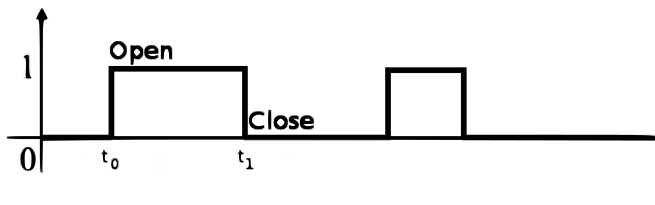
\includegraphics[width=\linewidth,totalheight=\textheight,keepaspectratio]{gfx/graph2.png}
      \caption{Sémantique des rôles.}
      \label{fig:semofroles}
\end{figure}

En pratique, pour fournir cette sémantique temporelle à l'application, 
l'implémentation d'un rôle doit être filtrée pour isoler les séquences de 
données atypiques (bruit). Par exemple, pour un rôle joué par un capteur de 
contact, s'il fournit deux valeurs true (ouverture) consécutives, l'implementation
filtrera habituellement la seconde valeur.

\section{Modèle d'infrastructure}\label{seq:fiabilite:model}
Les capteurs installés dans un domicile forment une infrastructure qui supporte 
les rôles requis par les applications déployées. 
La bonne implantation des rôles est critique pour la fiabilité de la 
sensibilité au contexte de cette infrastructure et donc des applications qui 
reposent sur cette infrastructure. 
Cette fiabilité va au-delà des tests unitaires de chaque rôle.

Pour adresser la fiabilité de l'infrastructure, nous proposons de construire un 
modèle de cette infrastructure qui peut être vérifié. Ce modèle ne prend pas 
uniquement en compte les rôles individuels, mais également leur conformité par 
des règles globales portant sur l'infrastructure de capteurs.

\subsection{Les évènements de rôle}\label{archi:algebra} 
La première étape pour expliciter le modèle d'infrastructure par un
ensemble de règles, est de délimiter le domaine des objets sur lesquels les 
règles pourront agir~: les évènements de rôle. Un évènement de rôle se compose de trois 
éléments~: (1) une interaction qui s'est produite (2) à une localisation donnée, 
(3) pendant une période de temps spécifique. Tout d'abord examinons la notion 
de période. Elle est définie en tant qu'intervalle délimité par deux horodatages. 
Ainsi~: 
\begin{displaymath}\label{archi:algebra:period1}
 \begin{array}{c} 
  Period = \mathds{N}^2\\
    \forall~p \in Period, p = <t_1, t_2>~and~t_1~<~t_2
 \end{array}
\end{displaymath}

Une période peut également être vue comme un ensemble de valeurs
de temps croissantes (ou d'instants), allant de $t_1$ à $t_2$, séparées chaque 
fois d'une seconde -- une granularité plus fine n'est pas 
nécessaire en pratique. Nous pouvons alors utiliser les opérations habituelles sur 
les ensembles pour opérer avec les périodes, comme $\subseteq, \supseteq$.

Enfin, un évènement de rôle est une interaction qui est arrivée pendant une 
période. L'ensemble d'interactions est définie par $Inter$ (\eg Présence, 
Ouverture, Utilisation). Un ensemble de localisations, $Loc$, spécifie 
les emplacements d'intérêt dans le domicile (\eg Cuisine, Salle de bain, Chambre). 
Les évènements de rôle sont donc définis comme suit.
\begin{displaymath}\label{archi:algebra:event}
  \begin{array}{c}
    e~\in~Event = Inter \times Loc \times Period \\
  \end{array}
\end{displaymath}

Lorsque l'infrastructure de capteurs surveille le domicile, elle produit des 
logs de données structurés en flux d'évènements de rôles, définis précédemment. 
Le log d'évènements de rôles est défini ainsi $log~\in~Log = \mathscr{P}(Event)$

\subsection{Formuler des règles}
Maintenant que les logs d'évènements de rôles sont définis et peuvent ainsi 
être manipulés, nous nous intéressons aux règles du modèle d'infrastructure. 
Ces règles sont exprimées par un ensemble de formules logiques dans le 
calcul de prédicats du premier ordre. Nous introduisons ces règles en examinant 
trois exemples de notre cas d'utilisation.

\myparagraph{Présence dans la cuisine.} Cette règle rend explicite la dépendance 
des capteurs dans la cuisine. En substance, nous voulons exprimer le fait que 
chaque interaction détectée, qui n'est pas un mouvement, doit être encadrée par 
une interaction de mouvement. Ce faisant, nous exprimons le fait que le capteur 
de mouvement dans la cuisine couvre toutes les autres interactions dans la 
cuisine (\eg porte de placard, machine à café). Une fois exprimée, cette 
sémantique assure la conformité des relevés de capteurs dans la cuisine.

Notre règle de présence dans la cuisine est définie ainsi~: 
\begin{displaymath}\label{archi:algebra:example}
  \begin{array}{c}
    \forall~<i, Kitchen, p>~\in~Log, i \neq Presence~ \Rightarrow \\
    ~~~~\exists~ <Presence, Kitchen, p'>~\in~Log,~p \subseteq p' 
  \end{array}
\end{displaymath}

\myparagraph{Portes restées ouvertes.} Nous supposons que dans un but 
d'assistance domiciliaire, une porte équipée d'un capteur de contact ne doit 
pas rester ouverte au-delà d'une certaine durée, notée $MAX$. Une telle règle 
s'applique typiquement sur la porte du frigidaire et sur la porte d'entrée 
parce que dans des conditions d'utilisation normales d'une maison, elles ne 
peuvent pas rester ouvertes très longtemps. La durée $MAX$ 
peut varier en fonction des préférences de l'utilisateur et du type de porte.

Cette règle est définie ainsi~:
\begin{displaymath}\label{archi:algebra:example2}
  \begin{array}{c}
    \forall~<Opening, l, p>~\in~Log \Rightarrow  \# p < MAX
  \end{array}
\end{displaymath}

Notons qu'une porte restée ouverte très longtemps peut être associée soit à un dysfonctionnement du 
capteur (comme pour les portes suscitées, de l'entrée ou du frigidaire), soit à un oubli de l'utilisateur de fermer la porte si celle-ci 
n'est pas surveillée par une application déclenchant une notification de 
sécurité. Par exemple, la porte du placard de notre cas d'utilisation est 
surveillée uniquement pour rappeler à l'utilisateur de préparer ses repas, et non pas pour 
lui rappeler qu'elle est restée ouverte. 

\myparagraph{Non omniprésence.} Certaines règles de conformité peuvent être 
spécifiques à un certain domaine d'application. Par exemple, 
nos recherches en informatique ubiquitaire sont principalement concentrées sur 
l'autonomie domiciliaire de personnes âgées vivant seules. Cette situation nous 
permet de définir la règle de conformité suivante: un rôle de présence ne peut 
pas être détecté simultanément à deux emplacements différents. La règle de non 
omniprésence est définie ainsi. 
\begin{displaymath}\label{archi:algebra:example3}
  \begin{array}{c}
    \forall~<Presence, l, p>~\in~Log \Rightarrow \\
     ~~~~\nexists~ <Presence, l', p'>~\in~Log,~l \neq l' \wedge ~p' \cap p \neq \emptyset
  \end{array}
\end{displaymath}

En pratique, définir des règles de conformité doit être associé à la fourniture d'instructions 
précises pour installer et positionner les capteurs dans le monde physique. 
Par exemple, la règle de présence dans la cuisine nécessite que la présence 
soit reconnue dans toute la cuisine. Une fois un domicile installé, les 
règles assurent la conformité entre l'installation et le modèle.

\section{Validation}\label{seq:fiabilite:validation}

Pour valider le concept de modèle d'infrastructure à base de règles,
nous présentons tout d'abord une architecture pour vérifier en continu qu'une installation 
est conforme à son modèle. Ensuite, nous décrivons une implantation de
cette architecture~; celle-ci nous a permis de valider l'approche expérimentalement.

\subsection{Architecture}
Globalement, l'architecture que nous proposons consiste à abstraire les lectures brutes de 
capteurs à travers une couche de rôles, alimentant à la fois les applications 
avec des valeurs de plus haut niveau, et les logs d'évènements de rôles utilisés par les 
règles de conformité du modèle d'infrastructure. Cette architecture est décrite 
en Figure~\ref{fig:archi}.

Les évènements de rôles sont traités simultanément par les applications et le 
module de vérification du modèle. Ce faisant, les règles de conformité peuvent être exécutées à la 
volée pour relever les erreurs quand elles apparaissent. Alternativement, les 
règles peuvent être exécutées hors ligne, sur des log déjà enregistrés, pour diagnostiquer des problèmes lorsque 
un opérateur est disponible pour de la maintenance.

\begin{figure}[!h]
  \centering
  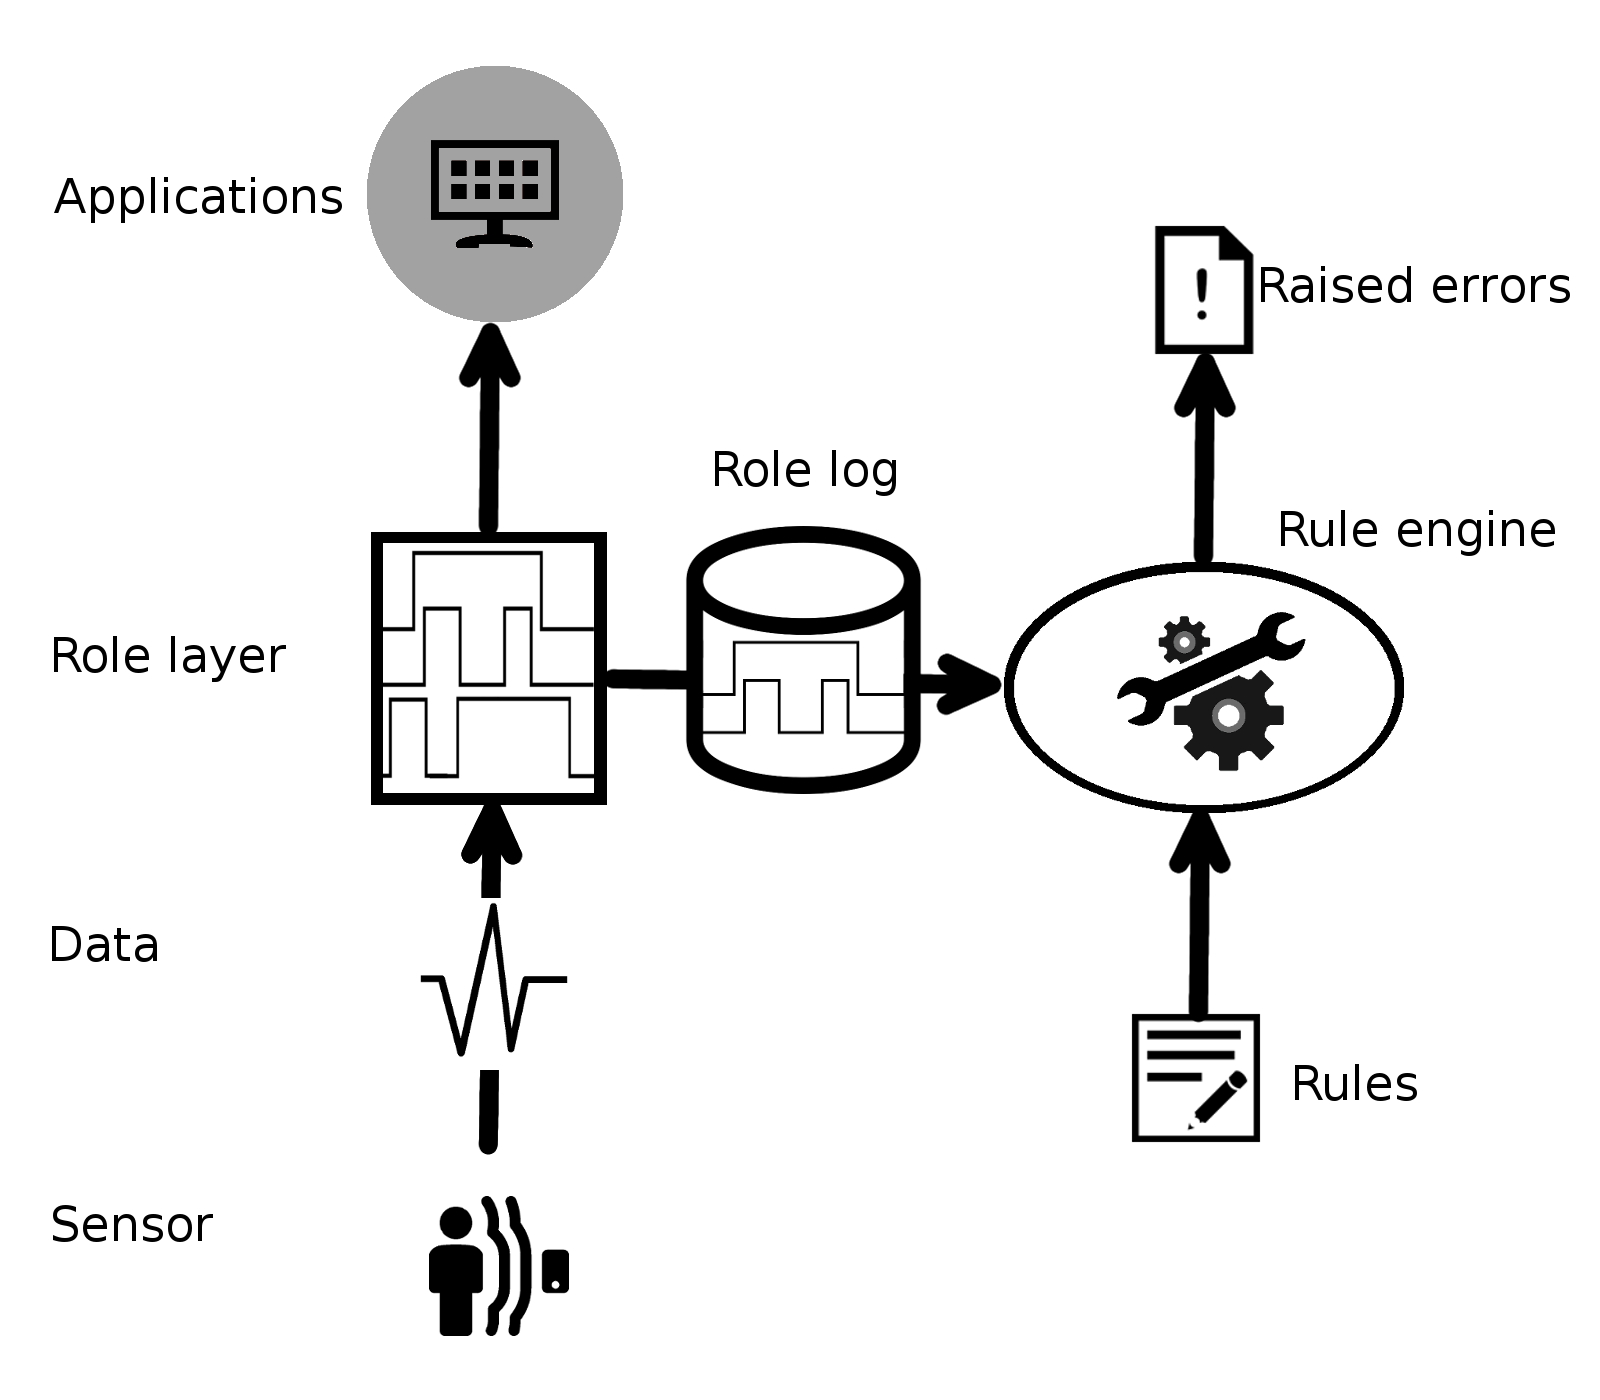
\includegraphics[width=\linewidth,totalheight=\textheight,keepaspectratio]{gfx/architecture.png}
  \caption{Architecture de notre approche de vérification continue d'une infrastructure par rapport à un modèle.}
  \label{fig:archi}
\end{figure}

Au-delà de la maintenance, les logs d'évènements de rôle peuvent aussi être 
précieux pour analyser l'évolution des activités quotidiennes des 
personnes âgées. En effet, ces logs permettent des analyses longitudinales qui 
peuvent, le cas échéant, révéler des dégradations du fonctionnement quotidien dues au 
vieillissement. Ces analyses permettent au professionnel d'adapter l'assistance 
en supprimant ou installant de nouvelles applications pour satisfaire l'évolution 
des besoins des utilisateurs. 

En outre, en faisant levier sur les logs d'évènements de rôle, la 
reconnaissance d'activités du quotidien peut être ajustée. Par exemple, le seuil 
de déclenchement des notifications peut être modifié pour prévenir la fatigue 
de l'utilisateur. De plus, ces logs peuvent servir pour rejouer des séquences 
d'interactions et déboguer des applications au comportement erroné.

\myparagraph{Règles.}
Les règles de conformité sont implantées sous la forme de prédicats Prolog, utilisant 
des opérateurs manipulant les évènements de rôles. 

\myparagraph{Analyseur de rôles.}
La plate-forme d'assistance utilisée pour valider notre approche ne fournissant 
pas la couche d'abstraction nécessaire pour produire les rôle, nous simulons 
cette couche dans notre implantation en utilisant un ``analyseur de rôles''. Ce 
composant construit un log d'évènements de rôles en transformant le log de 
lecture de capteurs et les informations associées (type de capteur, localisation, 
état et horodatage). Cet analyseur de rôle est implanté par un module C++.

\myparagraph{Moteur de règles.}
Ce module parcourt le log d'évènements de rôle produit par l'analyseur de rôles, 
et appelle un interpréteur Prolog pour exécuter chaque règle. De cette façon, 
quand une règle échoue, le moteur de règles identifie les évènements de rôle 
impliqués et produit une liste d'évènements de rôles non conformes avec les 
règles qu'ils ont fait échouer. Ce module est également implanté en C++. 
\newline

Le moteur de règles et l'analyseur de rôles totalisent plus de 2700 lignes de codes C++, 
pour transformer les données brutes de capteurs en évènements de rôles, et alimenter les règles en Prolog.

\subsection{L'expérimentation DomAssist}\label{seq:fiabilite:validation:domassist}
Le projet DomAssist\footnote{\url{http://phoenix.inria.fr/research-projects/homeassist}} 
vise à prolonger l'autonomie des personnes âgées dans leur propre 
domicile, en leur fournissant une plate-forme d'assistance domiciliaire avec des 
applications d'aide à la réalisation des activités quotidiennes. 
Des ergothérapeutes, psychologues et experts en vieillissement ont défini les 
activités à surveiller et l'ensemble des interactions à mesurer avec l'environnement.

Pour ce projet, deux types d'applications ont été définies~: (1) des applications 
pour surveiller les activités du quotidien et pour assister l'utilisateur quand elles 
n'ont pas été effectuées, et (2) des applications pour sécuriser le 
domicile ({\em e.g.,} porte d'entrée restée ouverte). Une première étude utilisateur a 
été conduite en recrutant 24 participants et en déployant à leur domicile notre 
plate-forme d'assistance domiciliaire pour une durée de neuf mois. Nous avons 
utilisé les données collectées durant cette première étude du projet DomAssist pour valider notre 
modèle d'infrastructure.

\subsection{Modèle}\label{validation:model} 
Les capteurs utilisés dans cette expérimentation permettent de mesurer douze 
interactions différentes avec l'environnement. Les interactions de présence sont 
mesurées avec des capteurs de mouvement, les ouvertures sont mesurées avec des 
capteurs de contact, et l'utilisation d'appareils électriques est mesurée avec 
des capteurs de consommation électrique. La configuration de DomAssist en terme 
de capteurs et leur rôles associés est résumée dans la Table~\ref{tab:domassist:role}.
\begin{table}[h!]
  \centering
  \begin{tabular}{|l|l|l|}
    \hline
    Room & Role & Sensor \\
    \hline
    \multirow{5}{*}{Kitchen} & Coffee maker in use & EM \\
    & Cabinet door open & CS \\
    & Fridge door open & CS \\
    & Microwave in use & EM \\
    & Presence & CS \\
    \hline
    \multirow{2}{*}{Entrance} & Door open & CS \\
    & Presence & MD \\
    \hline
    \multirow{2}{*}{Bathroom} & Shower in use & MD \\
    & Presence & MD \\
    \hline
    \multirow{2}{*}{Bedroom} & Dressing open & CS \\
    & Bedside lamp in use & EM \\
    & Presence & MD\\
    \hline
  \end{tabular}
\ \\ EM = Electric Meter, CS = Contact Sensor,\\ MD = Motion Detector.
  \caption{Rôles dans DomAssist.}
  \label{tab:domassist:role}
\end{table}

Pour des raisons pratiques, notre approche n'a pas pu être déployée au commencement 
de l'expérimentation DomAssist. 
% Nous avons donc appliqué notre 
% approche a posteriori. 
Notre modèle a donc été appliqué rétrospectivement pour 
vérifier la conformité du domicile de chaque participant en exécutant les règles 
sur les logs accumulés durant l'expérimentation.

En étudiant les conditions de l'expérimentation et nos rôles, nous avons 
spécifié les règles de conformité qui rendent explicites les conditions de 
l'étude~: les participants vivent seuls (règle de non omniprésence) 
et certaines interactions avec l'environnement doivent suivre un motif spécifique 
(porte restée ouverte). D'autres règles ne dépendent pas de l'objectif de l'étude 
et peuvent être généralisées. La règle d'inclusion de présence et ses 
raffinements (intersection de présence et besoin de présence) en sont des illustrations.
Examinons maintenant ces règles.

\myparagraph{Non omniprésence.}
Cette règle assure qu'un rôle de présence n'est pas détecté simultanément à deux 
localisations différentes. En pratique, en fonction de la réactivité des capteurs 
de mouvements utilisés pour la détection de présence, quelques brefs chevauchements 
peuvent survenir et doivent être ignorés. Typiquement, un détecteur de présence 
signale une absence avec une latence. Cette latence rend possible la
détection simultanée  de l'utilisateur dans deux pièces pendant quelques instants.

\myparagraph{Porte restée ouverte.}
Cette règle assure que la période d'un rôle d'ouverture de porte ne dure pas 
plus d'un certain temps (trois heures dans notre configuration). 
Notons que cette règle est exécutée sur les logs d'évènements, en complément
d'autres applications d'assistance qui peuvent réagir aussi 
à une telle situation. Par exemple, DomAssist inclut une application qui 
surveille la porte d'entrée. Cette application notifie l'utilisateur quand la porte est restée 
ouverte, sans surveillance pendant quelques minutes (la durée est configurée 
en fonction de l'utilisateur). Aussi, quand elle est appliquée aux logs 
de notre étude, cette règle détecte dans la plupart des cas des problèmes 
d'installation. 
% \cc je ne comprends pas la phrase suivante. Remplace "cela" par un mot et relis l'ensemble du paragraphe.
% Cependant, cette règle reste vrai même pour des portes non surveillées par des 
% applications de sécurité. 
Cette situation concerne également les portes non surveillées par des 
applications de sécurité (telle une porte de placard), ce qui s'explique par le fait que
les participants sont routinisés dans leurs
activités~\paulcite{bergua2013restriction} et n'ont pas déclinés  
cognitivement de façon significative durant l'étude.

\myparagraph{Inclusion de présence.}
Chaque pièce pour laquelle une interaction doit être détectée est équipée avec 
un détecteur de mouvement. Par conséquent, nous avons généralisé la règle de 
présence dans la cuisine à toutes les pièces~: toute interaction, qui n'est pas 
une présence, à une localisation donnée, doit être inclue dans un rôle de 
présence à la même localisation. 

\myparagraph{Intersection de présence.}
L'inclusion de présence peut être trop contraignante pour s'appliquer à 
certaines situations. Parfois, nous devons simplement nous assurer que la 
présence et d'autres interactions ont une intersections non nulle quand elle 
sont situées dans la même pièce. Une telle règle s'applique dans l'entrée du 
domicile, équipée d'un capteur de contact sur la porte d'entrée et un capteur 
de mouvement dans l'entrée (zone située à l'intérieur du domicile). 
En effet, si l'utilisateur ouvre la porte, que ce soit 
depuis l'extérieur ou depuis l'intérieur, les rôles de présence et d'ouverture ont une 
période de temps durant laquelle leur intersection est non-nulle.

\myparagraph{Besoin de présence.}
Pour s'assurer que le détecteur de mouvement est toujours actif même si il est 
mal positionné, nous introduisons la règle suivante~: chaque rôle, qui n'est pas 
une présence, doit être accompagné d'un évènement de rôle présence à la même 
localisation. Cette présence doit arriver au même moment plus ou moins dix minutes. 
Cette règle rend explicite le fait que le capteur de mouvement est toujours 
couplé avec un ou plusieurs autres capteurs dans notre configuration. La 
violation de cette règle indique principalement que le capteur de mouvement 
ne fonctionne pas correctement, probablement car il est toujours enregistré dans le système, 
mais n'émet plus aucune donnée.

\subsection{Méthodologie}\label{validation:methodology}
Nous avons collecté les logs des capteurs placés dans les habitations des 24 participants à 
l'étude. Ces participants sont âgés de 80 ans en moyenne et habitent seuls. Les 
données collectées couvrent une période de neuf mois. Cependant, des problèmes 
techniques (\eg accès internet, passerelle domotique, serveur) nous ont poussé 
à ignorer certaines périodes de temps~; ces problèmes peuvent être directement 
détectés par la plate-forme. Les logs de l'expérimentation ont également 
été nettoyés en éliminant les évènements de rôle non conformes 
pouvant être détectés par un mécanisme de tolérance aux fautes détectant 
les fautes de capteurs et de réseau, selon la classification définie 
par Chetan~\etal~\parencite{chetan2005toward}.
% simple système de surveillance de type
% heartbeat. 
% \cc mettre une citation et mentionner que c'est un mecanisme de tolerance aux fautes (a verifier)
%En effet, 
Par exemple, l'absence de signal de heartbeat, normalement émis par tout capteur, 
est détectée par les couches basses de la plate-forme et signalée comme un échec 
de communication avec le capteur.

Nous avons examiné le plan du domicile de chaque participant, spécifiant le placement 
et le positionnement des capteurs. Ce document a été utilisé pour 
diagnostiquer les problèmes quand des violations de conformités sont arrivées dans 
les logs. D'autres ressources ont été également disponibles pour diagnostiquer 
les violations, telles que les fichiers de suivi des interventions remplies par les 
professionnels chargés de faire passer des questionnaires à chaque participant
durant l'étude.

\subsection{Résultats expérimentaux}\label{validation:results}
Le modèle défini pour DomAssist permet de lever deux types 
d'anomalies~: (1) {\em les non-conformités permanentes} -- elles font réfèrence à une règle 
systématiquement transgressée, indiquant des non concordances permanentes entre 
l'infrastructure et le modèle~; (2) {\em les non-conformités émergentes}
-- elles correspondent à une règle qui est vérifiée la plupart du temps, mais échoue 
ponctuellement.

\myparagraph{Non-conformités permanentes.}
Dans un domicile, l'interaction d'ouverture est détectée pour la porte du 
placard de la cuisine, mais les règles {\em inclusion de présence} et 
{\em intersection de présence} échouent systématiquement. Cependant, 
la règle de {\em besoin de présence} n'échoue jamais, indiquant que la porte de 
placard est ouverte mais jamais couverte, ni même en intersection avec une interaction de présence dans la 
cuisine~; la présence est donc détectée à des moments proches mais disjoints de
l'interaction d'ouverture. La consultation des documents relatifs à cette 
installation ont montré que ce placard n'est pas localisé dans la cuisine mais 
dans une pièce attenante, comme montré en Figure~\ref{fig:map}. Cette situation 
montre un problème dans la définition du modèle pour cette
installation. Par conséquent, nous avons modifié le modèle de cette installation en y supprimant 
les règles d'inclusion de présence et d'intersection de présence. Nous
les avons remplacées par la règle besoin de présence, mieux adaptée à cette configuration.

Dans ce même domicile, un autre problème à été identifié~: la règle 
{\em inclusion de présence} échoue systématiquement sur le rôle d'ouverture du 
frigidaire, mais l'{\em intersection de présence} n'échoue jamais. Bien que le 
frigidaire soit localisé dans la cuisine, le capteur de mouvement utilisé pour 
mesuré la présence dans la cuisine, n'a pas été positionné pour couvrir 
l'ensemble de la cuisine, comme montré en Figure~\ref{fig:map}. 
Ce problème provient dans ce cas d'une erreur à l'installation et la solution
consiste simplement à changer le positionnement du capteur de mouvement. 

Nous avons observé la même configuration du placard de la cuisine situé en 
dehors de la cuisine, dans deux autres domiciles.

Généralement, ces types de problèmes surviennent quand la plate-forme d'assistance est 
déployée à large échelle. Dans ce contexte, les installations sont faites par 
un professionnel, et non par les chercheurs qui ont conçu la
plate-forme et qui possèdent un savoir implicite sur la bonne manière de déployer. Dans notre cas, 
même pour 24 domiciles, quelques installations ont été faites par des membres 
n'ayant pas ce savoir, et donc n'ont pas pu se conformés à certaines règles implicites.

\begin{figure}[!h]
  \centering
      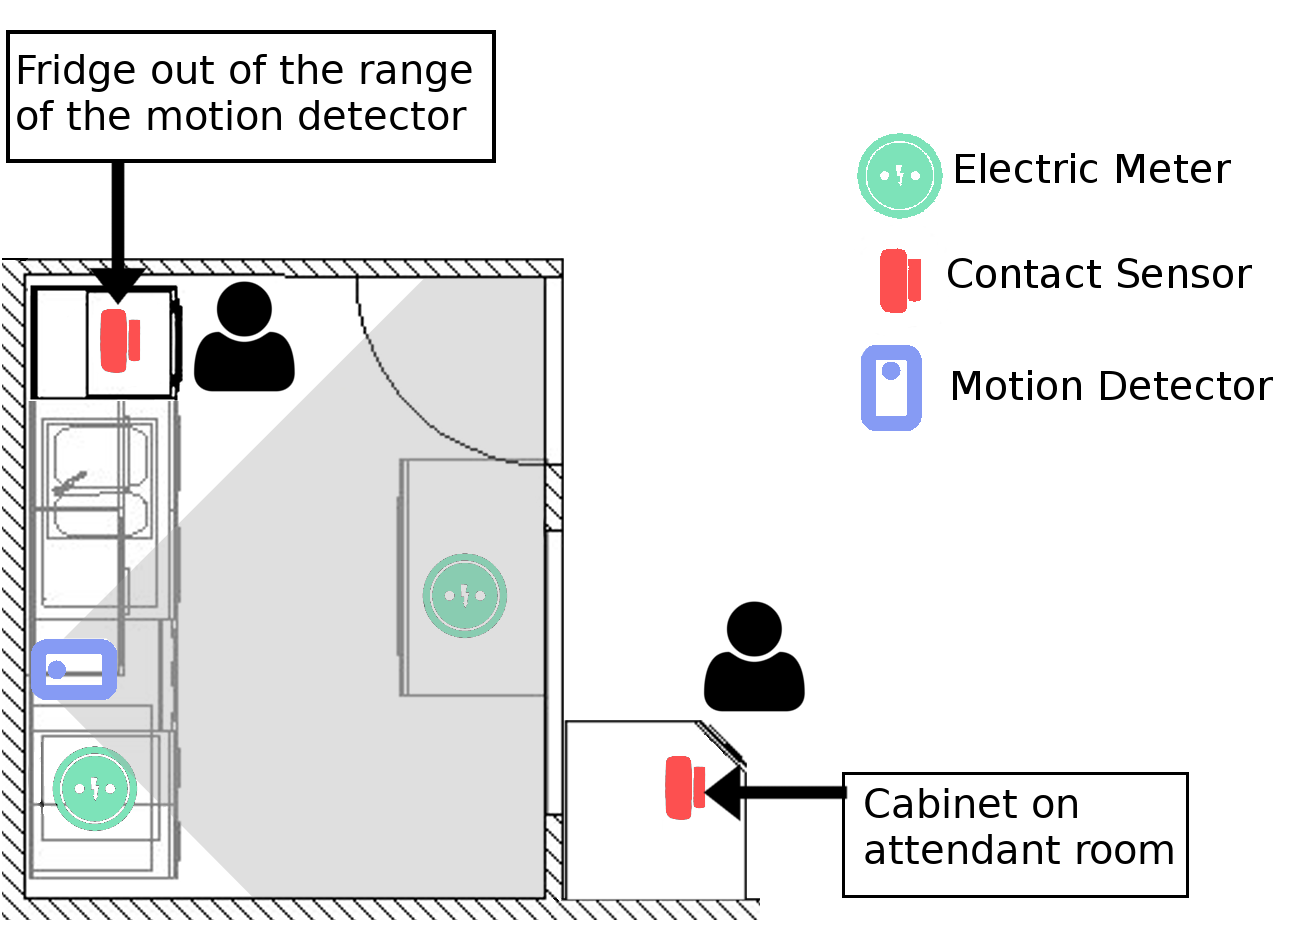
\includegraphics[width=\linewidth,totalheight=\textheight,keepaspectratio]{gfx/nconf2.png}
      \caption{Illustration de problèmes d'installation.}
      \label{fig:map}
\end{figure}

Si notre outil avait été utilisé dès la phase de déploiement, il aurait été 
possible de détecter les anomalies d'installation dès le départ, pendant 
l'installation ou dans les premiers jours d'exploitation. Par ailleurs, une 
fois déployées, des règles supplémentaires peuvent affiner les modèle pour 
prendre en compte des spécifications imprévues (\eg cuisine en forme de L). 
Une fois l'installation ou le modèle affiné, notre approche contribue à la détection 
d'anomalies au quotidien, en une période de fonctionnement normal.

\myparagraph{Non-conformités émergentes.}
Un motif de non concordance a été observé dans cinq domiciles à différentes 
périodes de temps. Pendant plusieurs jours, la règle {\em inclusion de présence} 
a été enfreinte par une absence de présence dans la cuisine causée par un 
capteur de mouvement qui dysfonctionnait. Dans chacun des cas, les règles 
d'{\em intersection de présence} et de {\em besoin de présence} étaient 
également transgressée durant ces périodes. Cette dernière règle montre 
qu'aucun rôle de présence n'a été reconnu durant les 20 minutes entourant cette 
violation. Les résultats de ces règles fournissent de précieuses informations 
pour trouver la cause des dysfonctionnement relevés. Il est alors raisonnable de 
supposer que la cause de cet échec des règles est un dysfonctionnement temporaire 
du rôle de présence. Nous pouvons supposer que le capteur de mouvement a pu être obstrué 
ou déplacé. 

Une situation similaire est arrivée dans l'entrée de deux autres domiciles~: la 
porte a parfois été ouverte, sans qu'aucune présence n'ait été détectée.

La {\em porte restée ouverte} a été observée dans quatre domiciles à différents 
endroits comme le frigidaire, le placard de la cuisine ou la penderie (\ie la 
porte est restée ouverte plus de trois heures). D'après les fichiers de suivi 
des interventions de l'expérimentation, les utilisateurs concernés ont été 
questionnés après quelques jours sur les comportements erronés des applications 
reposant sur ces interactions. Ils ont indiqué que les capteurs de contact 
étaient tombés. Les installations ont alors été réparées par les techniciens 
chargés des interventions. Notre modèle, si il avait été disponible durant 
cette expérimentation aurait permis de rapporter ces incidents, et de les 
solutionner plus rapidement. Cette réactivité est indispensable pour la pertinence 
des résultats des application sensibles au contexte. Elle fait toute la différence 
entre une application utile et une application qui harcèle l'utilisateur avec 
des notifications non pertinentes.

\section{Discussion}\label{sec:discussion}
Un modèle explicite d'une infrastructure est capable de détecter les 
dysfonctionnements du systèmes durant la phase d'installation ou pendant 
l'exploitation normale. Comme suggéré par certains de nos exemples, une fois 
une erreur détectée, quelques techniques de diagnostic peuvent être utilisées 
pour identifier les rôles qui sont la source de l'erreur.  

Premièrement, si plusieurs règles sont violées en même temps, et que ces règles 
concernent des ensembles de capteurs qui se chevauchent, il est alors probable 
que le rôle à la source de cette erreur soit à rechercher à l'intersection de 
ces ensembles. Par exemple, quand la règle {\em intersection de présence} 
échoue en même temps pour le rôle présence dans la cuisine et pour différentes 
interactions qui ne sont pas des présences (frigidaire, placard, \etc), 
%on peut 
%supposer que 
le rôle défaillant est 
probablement 
la présence 
dans la cuisine. 

Deuxièmement, concevoir une version raffinée d'une règle qui vérifie un ensemble 
de capteurs (ou est un sous-ensemble de la règle de base) peut s'avérer utile 
pour diriger la recherche d'un rôle défaillant ou d'un capteur qui dysfonctionne. 
Cette idée est illustrée dans notre modèle pour DomAssist. Il y a une chaîne 
de trois règles $R_i$ avec des conditions de moins en moins précises~:
{\em inclusion de présence}, {\em intersection de présence} et 
{\em besoin de présence}. Toutes ces règles sont du type 
$p \rightarrow q_i$ pour $(i=1..3)$ où le postulat $p$ est identique, mais la 
conclusion $q_i$ est de plus en plus faible. Il y a une implication tout au long 
de la chaîne, $R_1 \rightarrow R_2 \rightarrow R_3$~; ou inversement, quand une 
des règles échoue, les règles les plus fortes échouent également. Basé sur 
l'analyse des règles, nous pouvons définir un arbre de décision comme celui en 
Figure~\ref{fig:bdd} pour aider au diagnostic.

\begin{figure}[!h]
  \centering
      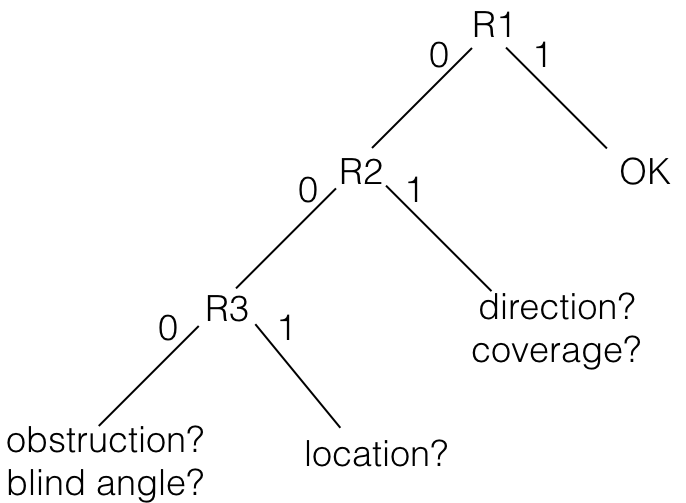
\includegraphics[scale=0.3]{gfx/bdd.png}
      \caption{Arbre de décision binaire aidant au diagnostic de la source d'une défaillance.}
      \label{fig:bdd}
\end{figure}

L'utilité de notre approche pour assurer continuellement la conformité d'une 
infrastructure va au-delà de la détection d'infrastructures défaillantes. 
Par exemple, un modèle d'infrastructure pourrait fournir un modèle de référence pour des applications 
disponibles dans un catalogue en ligne de type Appstore~: une application pourrait 
être installée uniquement lorsqu'elle est conforme au modèle d'infrastructure. 
En pratique, ce filtrage des applications au moment de l'installation pourrait remplacer
un certain nombre de tests qui sont nécessaires aujourd'hui pour chaque application déployée sur une installation
donnée, pourvu que le modèle couvre toutes les hypothèses requises par les applications.

\section{Conclusion}\label{sec:futurework}
Nous avons montré que les applications sensibles au contexte reposent 
fréquemment sur des suppositions implicites concernant l'infrastructure de capteurs. Ces 
suppositions se traduisent généralement en terme de programmation par des instructions conditionnelles qui 
polluent le code avec des préoccupations non fonctionnelles. Cette approche de programmation
défensive peut être évitée en exprimant ces suppositions, non pas dans le code 
des applications, mais en les factorisant dans un modèle explicite 
d'infrastructure de capteurs. Non seulement la violation d'une règle
du modèle d'infrastructure
permet d'alerter rapidement sur un dysfonctionnement de
l'installation, mais cette situation
contribue également à diagnostiquer le problème. 
Une telle approche permet de s'assurer de la fiabilité de la sensibilité au 
contexte des applications d'assistance domiciliaire. De plus, la définition du 
modèle permet de fourmuler des instructions détaillées quant à l'installation 
des capteurs dans le domicile, rendant ce dernier sensible au contexte.


% Our approach has been implemented in the context of an assisted living platform, running a set of applications dedicated to assist senior users. Our tool was applied to real sensor data collected during a 9-month field study, consisting of 24 participants aged 80 on average. The results show that some latent installation mistakes could have been found at installation time, using our model. Furthermore, several sensor problems that occurred during operation could have been detected on the fly and repaired more promptly to ensure the reliability of context-awareness applications.

% In future work, we will apply our method in a larger deployment consisting in hundreds of installations. This setting will allow us to quantify in more detail the improved reactivity in detecting emerging infrastructure issues, remotely diagnosing the underlying failure, and repairing the platform on-site. Another future work will consist of proposing log visualisation techniques and tools that contribute to identify new rules for the model by recognizing regular event patterns and anomalies. 
\chapter{Analyse de domaine}\label{chap:domain}
\begin{preamble}
Le chapitre précédent nous donne une fondation solide pour déployer des services contextuels dans une maison connectée, 
en assurant la fiabilité de son infrastructure de capteurs. 
Nous pouvons désormais nous intéresser au développement de ces services contextuels.
Pour cela, nous allons analyser dans ce chapitre un large éventail de services d'assistance domiciliaire 
dédiés aux personnes âgées, en considérant la variété des besoins des 
intervenants. 
%Ces services sont installés sur la plate-forme d'assistance domiciliaire DomAssist-2 déployée chez 129 personnes 
%âgées vivant seules et âgées de 82 ans en moyenne~\paulcite{consel2017homeassist}. 
Cette analyse permet d'identifier les concepts communs et les variations
entre différentes couches de services déployés et utilisés au quotidien,
pour en extraire des concepts clés et des opérations spécifiques aux
traitements sensibles au contexte\footnotemark{}\footnotetext{Ce travail à fait l'objet d'une soumission~:~\fullcite{carteron2017domain}.}.
\end{preamble}
\chpsummary{Aperçu}
{
{\em DomAssist} Présentation d'une expérimentation écologique large échelle sur laquelle nous nous appuyons pour notre analyse.;
{\em Analyse de domaine} Identification des concepts clés, des opérations spécifiques et des besoins communs aux services sensibles au contexte.
}

Les services d'assistance dédiés au maintien à domicile
des personnes âgées sont encore un domaine émergeant et le chemin vers l'adoption
reste un sujet d'étude~\paulcite{kaye2017making}. La littérature
comporte encore peu d'articles concernant le déploiement de solutions
d'assistance dans de vrais domiciles~\paulcite{kaye2011intelligent}. 
Cependant, nous avons pu faire levier
sur le projet DomAssist pour conduire notre analyse du domaine.

\section{Enjeux d'une expérimentation écologique à large échelle}\label{domain:expe}
L'étude pilote de la plate-forme, DomAssist, présentée dans le 
Chapitre~\ref{cha:fiabilite}, a donné des résultats 
encourageants quant à l'acceptabilité de la technologie, par un groupe de 24 
utilisateurs, âgés de 80 ans en moyenne, pendant une durée 
de 9 mois. D'un point de vue technologique, cette expérimentation, était une 
première confrontation aux difficultés et contraintes d'un déploiement écologique.
Nous avons donc conçu l'approche présentée dans le Chapitre~\ref{cha:fiabilite}
pour nous assurer du bon fonctionnement de l'infrastructure de
capteurs, lors de son installation et durant son exploitation, et pour garantir la consistance des 
services d'assistance.

Faisant suite à l'étude pilote, une nouvelle expérimentation
d'autonomie domiciliaire des personnes âgées est en cours à plus large
échelle, couvrant un plus grand nombre d'utilisateurs pour une durée
de 12 mois\footnote{\url{http://phoenix.inria.fr/research-projects/homeassist-500}}. La plate-forme est actuellement déployée chez 129
personnes vivant seules et âgées de 82 ans en
moyenne~\paulcite{consel2017homeassist}.  Cette expérimentation est
construite en lien étroit avec les acteurs du domaine de l'autonomie
domiciliaire des personnes âgées. Ainsi, la conception et la mise en
place des services ont impliqué tous les acteurs~: utilisateurs,
aidants, ergothérapeutes, psychologues, experts en facteurs humains,
techniciens d'installation et de maintenance et informaticiens.  Le
modèle d'assistance qui en résulte offre des services dédiés à des
tâches variées comme les rappels de rendez-vous, la surveillance
d'activités du quotidien ainsi que leur rappel si elles ne sont pas
effectuées, la sécurisation de l'utilisateur, ou encore le bilan
quotidien des activités.  L'analyse des données recueillies permet
d'évaluer et d'adapter l'assistance en fonction de chaque utilisateur
et de ses dégradations éventuelles.

Cette étude à large échelle offre de nombreux avantages pour
construire notre analyse du domaine~: (1) elle est déployée dans des
environnements réels~; (2) elle constitue un soutien pour le maintien
à domicile de personnes âgées avec des utilisateurs fragiles ayant des
besoins immédiats. La précédente expérimentation avait pour but
principal d'ajuster et de valider la plate-forme DomAssist en tant que
plate-forme d'assistance domiciliaire, en n'incluant pas
d'utilisateurs avec un statut fonctionnel trop dégradé. La nouvelle
étude est ouverte à plus d'utilisateurs et permet donc d'élargir les
services d'assistance. (3) L'étude conduite est suffisamment longue
pour que les problèmes de maintenance et d'évolution doivent être
traités avec réactivité. (4) La plate-forme est déployée à une échelle
suffisamment large pour que l'administration des domiciles ait besoin
d'être supportée par des services. Avec un tel nombre de domiciles
installés, il est indispensable de disposer de services qui signalent
automatiquement les cas de dysfonctionnements, afin que des
dispositions soient prises au plus tôt. (5) En conséquence, les
services existants reflètent un large éventail de besoins exprimés par
les intervenants.  Nous disposons maintenant non seulement d'une large
gamme de services d'assistance domiciliaire, mais également de services
relatifs à la maintenance et la supervision de l'infrastructure de
cette assistance.

\subsection{Des services d'assistance}
Une étude de besoins, conduite auprès de personnes âgées vivant seules
et de leurs aidants, a permis aux experts en vieillissement,
psychologues et ergothérapeutes de formuler un cahier des charges des
services d'assistance à développer et au degré de personnalisation
indispensable au fonctionnement de ces services.  Comme évoqué plus
haut, la plate-forme propose trois catégories de services
d'assistance~: le support des activités du quotidien, la sécurité de
l'utilisateur et ses interactions
sociales~\paulcite{consel2017homeassist}. Les services d'assistance
sont développés en Java en utilisant une méthodologie de conception
outillée basée sur la paradigme {\em Sense Compute
  Control}~\paulciteseparate{bertran2014diasuite,cassou2012toward}.

Les services sont disponibles dans un catalogue d'applications en
ligne à la manière de ce qui est proposé de nos jours pour les
smartphones. Il est alors aisé d'adapter l'assistance fournie par la
plate-forme en supprimant ou ajoutant des applications en fonction de
l'évolution des besoins de l'utilisateur. Les applications peuvent
également être personnalisées en fonction de l'utilisateur. Par
exemple, un paramètre d'installation permet de définir la durée de
l'ouverture de la porte d'entrée sans surveillance, avant qu'une
alerte soit envoyée.

\subsection{Infrastructure}
La plate-forme DomAssist se compose d'une architecture client-serveur.
Le serveur instancie autant de machines virtuelles qu'il y a de
domiciles équipés de DomAssist. 
Chaque machine virtuelle permet d'exécuter les services d'assistance sélectionnés par 
l'utilisateur et les aidants.
Les services d'assistance sont alimentés avec les données de mesure d'interactions via Internet et une 
passerelle domotique déployée dans le domicile installé.
La passerelle centralise les informations en provenance des capteurs, installés 
aux endroits stratégiques du domicile pour surveiller les activités.
La passerelle relaie également les actions commandées par les services à 
destination des actionneurs.
Cette architecture est illustrée en
Figure~\ref{fig:archidomasssit}. %\cc Cette figure n'illustre pas du tout le propos. Je propose de la retirer
\begin{marginfigure}%[-2.54cm]
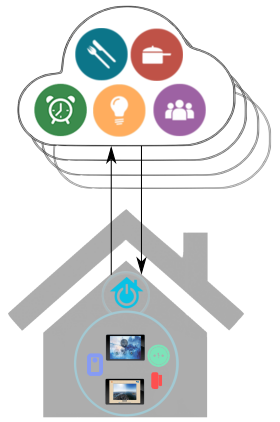
\includegraphics[width=\linewidth,totalheight=\textheight,keepaspectratio]{gfx/archi_domassist}
\caption{Illustration de l'architecture de la plate-forme DomAssist.}
\label{fig:archidomasssit}
\end{marginfigure} 

Dans l'étude DomAssist, un domicile typique est pourvu de quatre
capteurs de contact (porte d'entrée, frigidaire, armoire, \etc), six
détecteurs de mouvements (zone de l'entrée, cuisine, salle de bain,
\etc), et deux capteurs de consommation électrique, qui peuvent
également allumer et éteindre les appareils qui y sont branchés
(chemin lumineux, micro-onde, machine à café, \etc). Le nombre et le
type de capteurs/actionneurs peut varier en fonction de la
configuration du domicile et des activités à surveiller. Enfin, le
domicile est équipé avec deux tablettes. La première, une tablette
fixe, est placée à un endroit central dans le domicile et est toujours
alimentée électriquement. Cette tablette est dédiée aux interactions
de la plate-forme avec l'utilisateur via les notifications émises par
les applications d'assistance, qui alertent l'utilisateur d'une
situation donnée (\eg porte d'entrée ouverte et non surveillée depuis
un certain temps)~\paulcite{consel2015unifying}.  La seconde tablette,
dont la mobilité est autorisée, est utilisée pour les activités
sociales. Elle dispose notamment d'une application de gestion
simplifiée du courrier électronique, avec synthèse vocale. D'autres
applications de communication et des jeux collaboratifs sont également installées.
La Figure~\ref{fig:mapdeployed} montre un exemple de domicile équipé.

\begin{figure*}[]
  \centering
      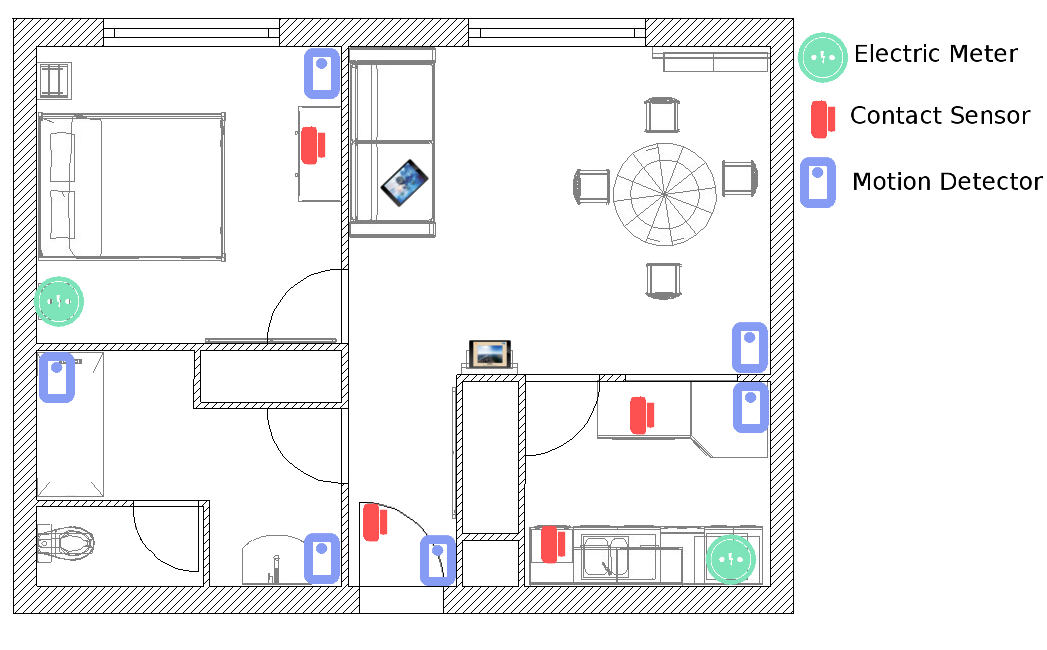
\includegraphics[width=\linewidth,totalheight=\textheight,keepaspectratio]{gfx/Map.png}
      \caption{Exemple de domicile déployé avec son installation de capteurs.}
      \label{fig:mapdeployed}
\end{figure*}


%**********************************************
\section{Scénarios pour le maintien à domicile}\label{domain:scenario}
Les services proposés par les applications disponibles sur la
plate-forme DomAssist concernent l'assistance domiciliaire. Cependant,
il existe de nombreux autres services nécessaires au fonctionnement de
la plate-forme, notamment sa maintenance (\eg infrastructure de
capteurs, infrastructure logicielle, réseau, \etc), qui vont
influencer le bon fonctionnement des services d'assistance.  Ces
services {\em annexes} sont instanciés, non pas directement au sein de
la plate-forme DomAssist en tant qu'applications disponibles, mais avec différents framework spécialisés
(\eg surveillance de la communication réseaux, charge des serveurs,
état des batteries des capteurs, état de l'infrastructure de capteurs,
\etc).

Pour définir quels sont les besoins des intervenants en matière de
services, nous avons recours à la plate-forme d'assistance déployée à
large échelle, aux intervenants ayant contribué à la définition de
services d'assistance, et aux intervenants participant à son
exploitation.  À partir de cet ensemble d'expertise, nous décrivons
dans la Table~\ref{scenario-fig}, quelques scénarios illustrant la
variété d'intervenants et la variété de préoccupations nécessaires au maintien à
domicile de personnes âgées, lorsque des services d'assistance sont
sensibles au contexte.


\begin{table*}[!h]
\begin{small}
\begin{tabular}{| p{2cm} | l | p{2.3cm} | p{7.5cm} |} \hline
{\bf Stakeholder} & {\bf Domain} & {\bf Name} & {\bf Description} \\ \hline \hline
Older adult& Safety & Door Alert & Entrance door \uline{is open} and  \uline{is unattended} \dotuline{for 5 minutes} \\ \hline
Caregiver & Daily Activities 
       & Reheating  A Frozen Meal 
          & Freezer \dashuline{gets used} and stove \dashuline{gets turned on} \dotuline{within 10 minutes} or Freezer \dashuline{gets used} during stove \uline{is on},
during \uline{lunch time} (or dinner time) \\ \hline
 Home Technician
               & Maintenance & Presence Dependency 
                  & The cupboard \dashuline{gets opened} in the kitchen, while a presence in the kitchen \uline{is false} \\ \hline
Home Technician
   & Maintenance 
        & Communication Failure 
             & A sensor \uline{fails to communicate} \dotuline{for 24 hours} %and its status does not \dashuline{get updated} 
\\ \hline
\end{tabular}
\end{small}
\vspace{5mm}
\label{scenario-fig}
\caption{Example de scénarios de services d'assistance.}
\end{table*}

Le premier scénario concerne la sécurité de l'utilisateur. Ce scénario
surveille la porte d'entrée pour s'assurer qu'elle ne reste pas
ouverte trop longtemps sans être surveillée.  Le deuxième scénario
implique à la fois l'utilisateur et l'aidant. Il illustre un besoin
exprimé par les aidants, en fournissant un service qui rappelle à
l'utilisateur une routine du quotidien, dans le cas où il ne l'aurait
pas réalisée (dans l'exemple, la préparation du repas). La formulation du
scénario est déterminée par l'utilisateur qui va définir lui-même la
façon dont il effectue ses routines quotidiennes.
Les deux derniers scénarios concernent des besoins exprimés par les techniciens 
pour garder opérationnels les domiciles sensible au contexte. 
Le premier scénario de maintenance détecte l'utilisation d'un placard sans que 
celle-ci soit recouverte par la détection d'une présence. 
Le second scénario de maintenance détecte quand la passerelle échoue à 
communiquer avec un capteur~;
cette situation se produit lorsque le capteur n'a plus de batterie ou dysfonctionne.

Ces scénarios offrent un aperçu des types de services sensibles au contexte 
nécessaires pour le maintien à domicile de personnes âgées. 
Ces services fournissent directement une assistance ou servent de support au 
bon fonctionnement de la plate-forme.
Certains services tels que ``Door Alert'', peuvent convenir à la plupart des 
utilisateurs. En revanche, d'autres services, typiquement les services concernant 
les activités du quotidien, nécessitent un certain degré de personnalisation pour 
être efficaces. Ceci est illustré par l'activité de préparation de repas et 
le scénario ``Reheating a Frozen Meal''.

De même, ``Communication Failure'' peut s'appliquer à n'importe quel 
domicile sensible au contexte, alors que ``Presence Dependency'' demande 
d'instancier les règles en fonction de la localisation des capteurs. 

Il est à noter que la formulation de certains scénarios, principalement les scénarios de sécurité de la personne ou les scénarios de maintenance, décrit des situations anormales. Par exemple, pour le scénario de ``Presence Dependency'', la situation normale serait décrite ainsi~: {\it ``Quand le placard est est ouvert dans la cuisine, la présence dans la cuisine est vraie''}. Or, dans ces cas là, le but de ces scénarios est d'identifier les situations inhabituelles, c'est donc ces situations qu'ils doivent décrire.

Une autre observation frappante est que certains services de maintenance reprennent directement des règles
qui faisaient partie du modèle d'infrastructure des capteurs, décrit dans le Chapitre~\ref{cha:fiabilite},
sauf qu'elles sont maintenant formulées par la négative, pour chercher les situations non-désirées,
comme expliqué ci-haut. En fait, {\em toutes} les régles du modèle explicite d'infrastructure peuvent
être ainsi exprimées comme des services d'acquisition de contexte, où le contexte concerne alors
les dysfonctionnements de l'infrastructure. Ainsi, le spectre des services contextuels dans une
maison connectée inclut comme un sous-ensemble le modèle d'infrastructure, dans le spectre bien plus large 
des services destinés à tous les intervenants de l'assistance domiciliaire.

\section{Analyse de commonalités et variabilités}\label{domain:commonvar}
Les scénarios définis nous permettent de faire une étude de commonalités et de variabilités.

\subsection{Commonalités} 
Tous les services se réfèrent à une notion d'{\em environnement} dans 
lequel sont effectuées les mesures. Ces mesures observent des interactions 
qui peuvent se passer soit dans l'environnement physique (\eg un mouvement détecté), soit dans 
l'environnement numérique (\eg un rappel d'évènement délivré par un agenda). 
Concernant ces mesures de l'environnement, nous avons identifiés deux concepts 
récurrents dans les scénarios étudiés~: les évènements et les états.
Un {\em évènement} définit une mesure de l'environnement au moment où 
l'interaction correspondante se produit (\eg une porte {\em devient} ouverte/fermée) -- les 
évènements sont soulignés avec des pointillés dans les scénarios de la Table\ref{scenario-fig}.
Un {\em état} exprime l'accès au statut courant d'une mesure préalable de l'environnement
%la persistance d'un évènement dans le temps 
(\eg la porte 
{\em est} ouverte/fermée) -- les états soulignés avec une ligne pleine dans 
la Table~\ref{scenario-fig}.
Ces deux concepts d'état et d'évènement permettent donc d'exprimer 
soit le moment où une interaction se produit, pour les évènements, soit
le statut d'une interaction déjà produite qui persiste dans 
le temps, pour les états.

Il est possible également d'identifier dans les scénarios, des concepts de 
{\em composition}. Spécifiquement, la combinaison de mesures d'environnement 
peut définir un {\em ordre} dans lequel les interactions doivent arriver et 
la {\em durée}, tant des interactions que des compositions -- ces contraintes 
sont soulignées avec des points dans la 
Table~\ref{scenario-fig}.

\subsection{Variabilités} 
Les mesures environnementales peuvent être réalisées 
par une variété d'entités, matérielles (\eg capteurs), logicielles (\eg agenda), 
locales (\eg porte), distante (\eg nouvel email), \etc 
Le niveau d'abstraction varie énormément selon les mesures environnementales. 
Par exemple, un évènement peut être produit par un capteur, sitôt qu'un 
mouvement est détecté dans l'entrée. Parallèlement, cette même interaction 
peut servir pour être agrégée avec d'autres évènements et produire un évènement
``rentrée au domicile''. 
Plusieurs contraintes d'ordre sont possibles pour la composition des 
interactions. Une interaction peut en {\em précéder} une autre, une interaction 
peut se produire {\em durant} une autre, et une interaction peut en {\em chevaucher} une 
autre. Cependant, toutes ces contraintes ne sont pas applicables à tous les types 
d'interactions (\ie évènements et états). Par exemple, seulement deux états 
peuvent se chevaucher, alors que les évènements ne peuvent pas se
chevaucher à cause de leur nature ponctuelle.
% dans la pratique cette situation suppose deux interactions strictement simultanées.

\subsection{Concepts spécifiques au domaine}
%Reccurrence dans les séquences à detecter

Suivant cette analyse, nous pouvons d'ores et déjà exprimer certains
concepts.  Nous retrouvons un modèle d'environnement, comme évoqué en
Section~\ref{seq:fiabilite:cas}, avec des informations sur
l'interaction (le type d'interaction mesurée, sa localisation,
la valeur mesurée, la positionnement dans le temps) et les niveaux
d'abstraction d'une interaction (\eg physiques, logiciels, \etc).
%(\eg état du capteur, type d'interaction mesurée, localisation de l'interaction, timer, agenda, etc).
Il est maintenant possible de définir plus précisément le concept d'évènement et d'état~:

\myparagraph{Évènement~:} un changement de valeur, pour une entité mesurée, qui se produit à un moment donné. 

\myparagraph{État~:} Une valeur qui subsiste pendant une période. L'état débute à un moment donné et finit à un autre moment.

Pour composer ces états et évènement dans le temps, nous avons extrait de notre analyse des opérateurs de composition (\eg précédence, chevauchement, \etc).

\section{Besoins communs}\label{domain:needs}
L'analyse des services d'une plate-forme d'assistance domiciliaire met en évidence certaines contraintes indispensables à l'exploitation des services. Du fait de leur sensibilité au contexte, et leur objectifs parfois critiques dans l'assistance domiciliaire (\eg sécurité, maintenance, \etc), les services doivent être capables de réagir rapidement aux mesures d'environnement qu'ils traitent.

De plus, des services avec des objectifs différents doivent pouvoir accéder aux mêmes données pour effectuer des traitements différents.
La variété d'intervenants et la variété de leur expertise impliquent une forte hétérogénéité de données qu'il faut exprimer en terme d'état et d'évènements.

Les services expriment un ensemble d'interactions qui peut revenir de façon récurrente dans le flux d'évènements d'interactions. Par exemple, les évènements décrivant l'activité de préparation d'un repas reviennent typiquement tous les jours. Par conséquent, un service vérifiant que l'activité à été effectué doit être testé de manière récurrente.

Comme observé, il y a une forte composante temporelle dans l'expression des services. Tant pour expliciter la durée de la persistance d'un état, que pour exprimer de simples relations entre états/évènements et la durée de cette relation, cette composante temporelle doit être partie intégrante de l'expressivité des services sensibles au contexte.

La variété d'intervenants implique également autant de manières de formuler un scénario de service.
Les scénarios exprimés par les intervenants doivent couvrir l'ensemble des services nécessaires à une plate-forme d'assistance de maintien à domicile des personnes âgées. Il faut donc être capable de proposer une solution permettant d'exprimer ces services en couvrant leur spectre d'expertise et d'objectifs. Cependant, malgré l'hétérogénéité des données captées et malgré la large variété des besoins entre les intervenants des différents domaines d'expertise, ces services sensibles au contextes agencent des concepts communs qui permettent d'uniformiser leur formulation et leur traitements.

\chapter{Maloya : Un langage spécifique dédié aux services sensibles au contextes}\label{sec:dsl}
\begin{preamble}
Ce chapitre présente notre approche dédiée au domaine de l'assistance domiciliaire. Dans un premier
temps, nous décrivons l'architecture logicielle sous-jacente à notre approche. Ensuite, nous
introduirons un langage dédié pour développer des services sensibles au contexte
%\footnotemark{}\footnotetext{Ce travail à fait l'objet d'une soumission~:~\fullcite{carteron2017domain}.}
. 
\end{preamble}
\chpsummary{Contributions}
{
{\em Architecture logicielle} Un architecture qui couvre les besoins d'unification de données hétérogènes et d'exécuter des services en continu sur le flux d'évènements. ;
{\em Langage dédié} Un langage spécifique pour développer un large spectre de services sensibles au contexte, avec un haut niveau d'asbtraction et un traitement uniforme de sources de données hétérogènes.;
{\em Validation} redéfinition de 55 services, couvrant les besoins de tous les intervenants d'une plate-forme d'assistance pour le maintien à domicile de personnes âgées.
}

Sur la base de l'analyse de domaine présentée dans le chapitre précédent, 
nous somme en mesure de proposer un langage dédié aux services sensibles au 
contexte, appelé Maloya, ainsi que l'architecture logicielle sur
laquelle repose ce langage~:
\begin{itemize}
\item Notre architecture logicielle  est {\em centrée données}, en unifiant des sources 
hétérogènes de données, que ce soit en provenance de capteurs matériels ou de capteurs logiciels.
%fournir 
Elle fournit à l'ensemble des services une vue canonique des données mesurées. Ainsi, cette
forme canonique couvre d'une part, les
services de maintenance requérant l'état bas niveau des capteurs, et d'autre part, 
les services spécifiques aux aidants nécessitant des mesures d'activités de haut 
niveau. 
\item Le langage dédié Maloya fournit à la fois un cadre 
conceptuel et des outils pour concevoir et développer des services domiciliaires 
pour les personnes âgées. Notre langage est {\em orientée données} avec des services définis en 
terme de règles traitant des évènements et des états, et des opérateurs pour les combiner. 
%Pour unifier les source hétérogènes de données, des composants matériels aux 
%composant logiciels, notre approche promeut un paradigme ``centré données'' 
%et ``orienté données''. 
\end{itemize}

\section{Une approche dédiée au domaine de l'assistance domiciliaire}
Nous présentons ici les étapes principales de notre approche spécifique au domaine 
pour développer des services sensibles au contexte dédié au maintien à domicile 
des personnes âgées.

La fourniture d'un service sensible au contexte, selon notre approche, implique deux phases principales, illustrées en Figure~\ref{fig:functionalarchi}: 
\begin{itemize}
\item La phase de développement~: les intervenants définissent un service sous 
forme de règle en langage Maloya. Cette règle métier est ensuite compilée vers une règle de plus bas niveau en 
langage de traitement d'évènements. Les outils assistant le développeur de service lors de cette phase comprennent le 
compilateur et une interface de gestion des services.
\item La phase d'exploitation~: les services compilés sont exécutés sur les flux 
d'évènements provenant d'une maison sensible au contexte. Une fois mise en place, une règle est 
exécutée de façon à révéler chaque occurrence de la séquence d'évènements 
qu'elle décrit, jusqu'à ce que la règle soit supprimée, ou mise à jour. 
La phase d'exploitation est implantée par un analyseur d'évènements d'interaction qui 
transforme ces évènements en une forme canonique appelée {\em StreamEvent} 
(ou simplement, flux d'évènement, par la suite) pour alimenter un moteur de traitement d'évènements 
complexes (CEP). Ce moteur CEP est chargé de l'exécution des règles compilées sur le flux d'évènements.
%qui exécute les règles sur ce flux d'èvenements et retourner un signal lorsqu'une séquence d'évènements correspondant à une règle est identifiée dans le flux. 
\end{itemize}
\begin{figure*}[h]
\centering
  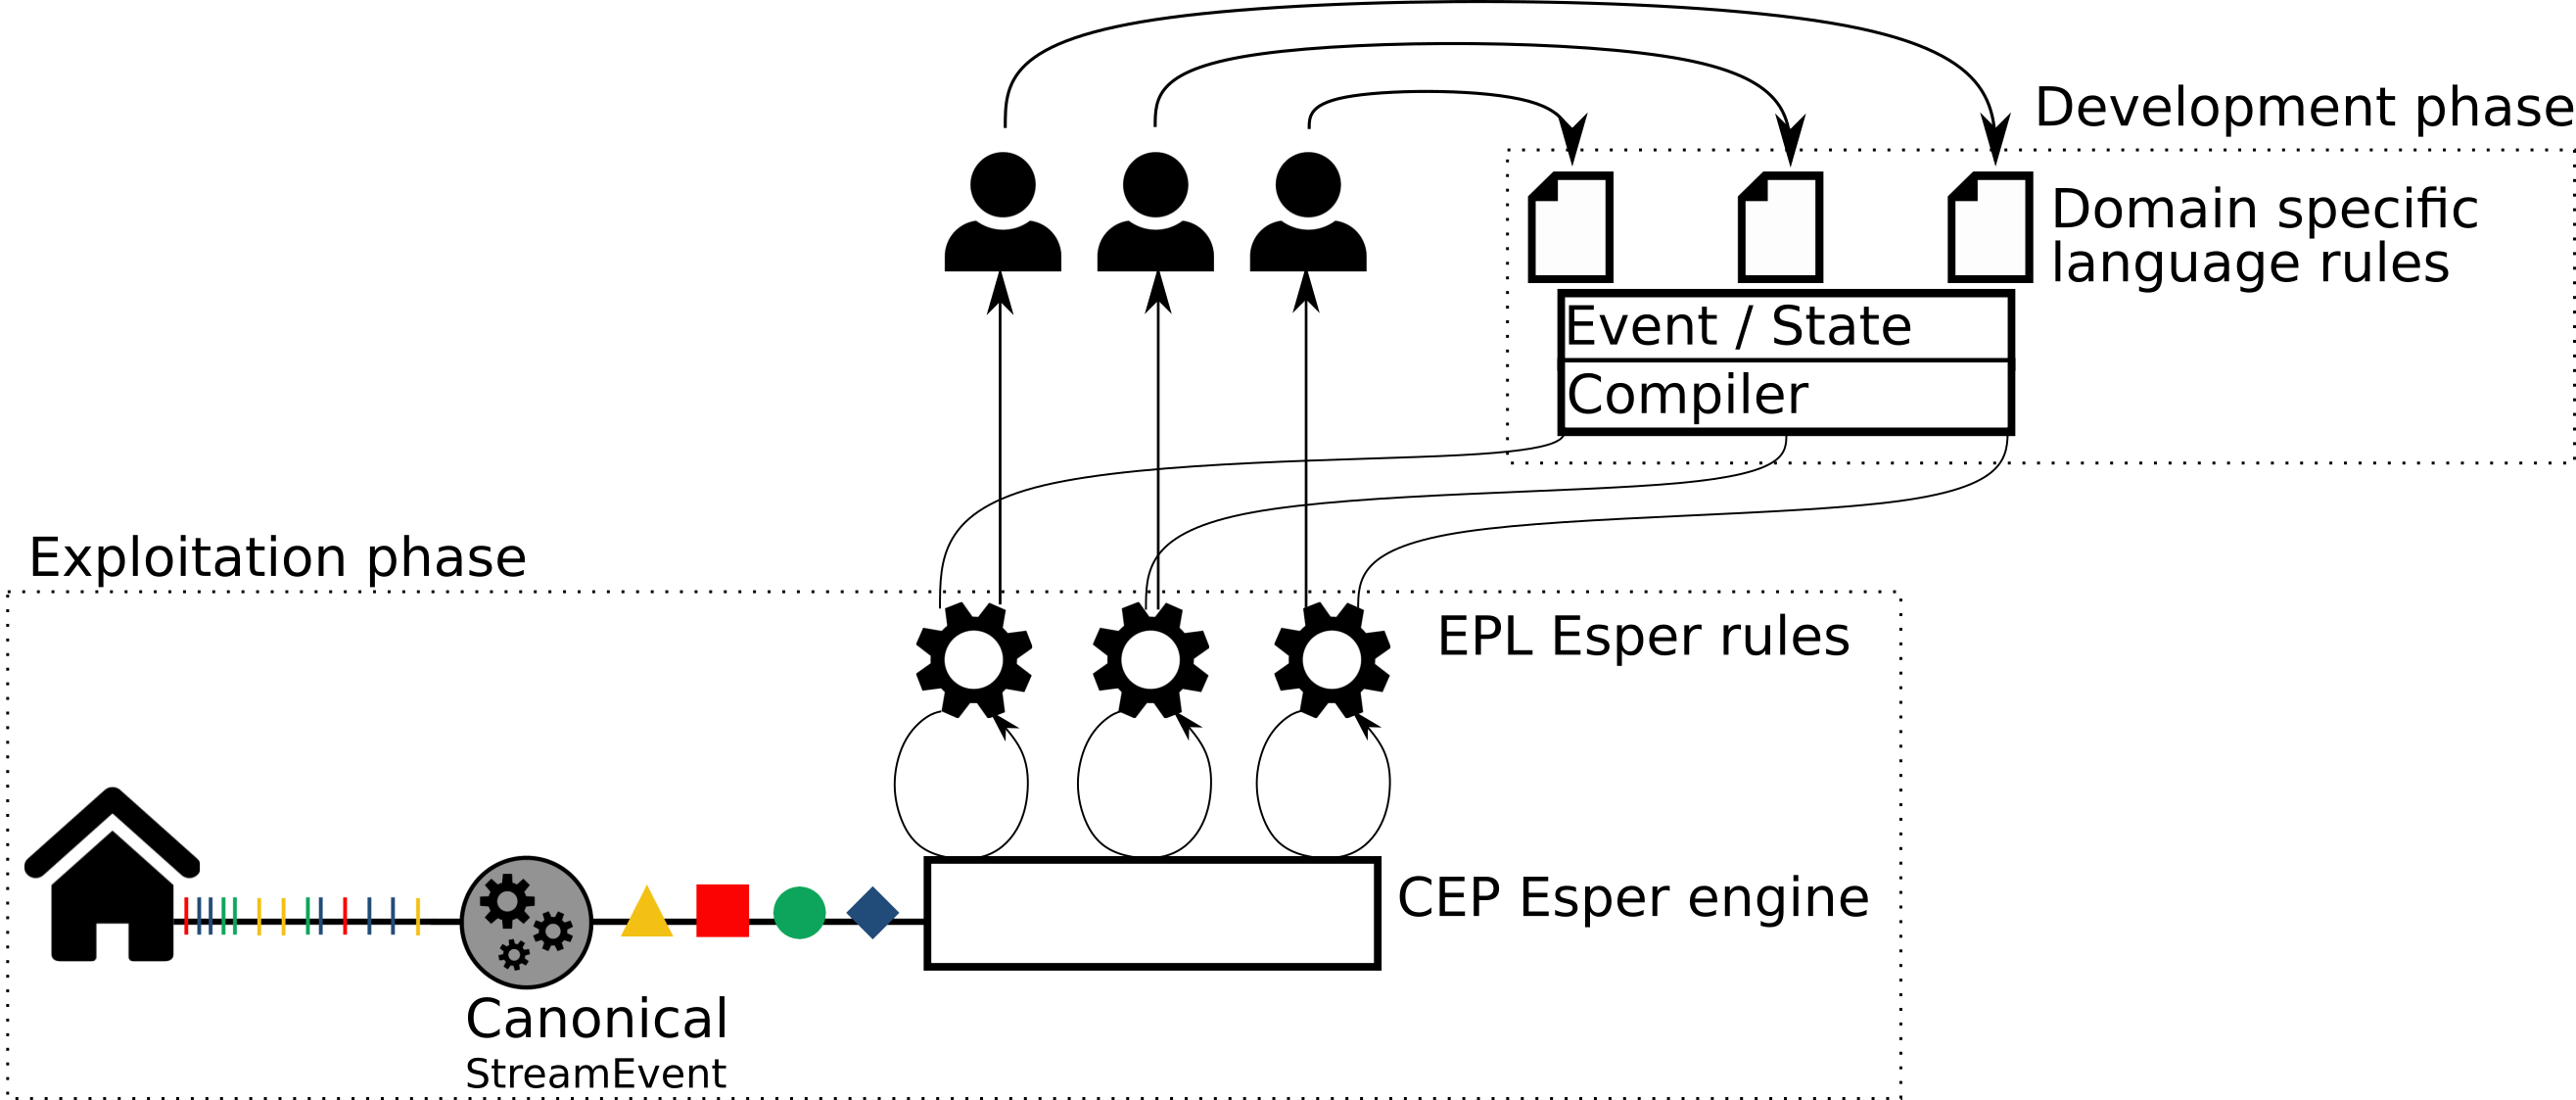
\includegraphics[width=\linewidth,totalheight=\textheight,keepaspectratio]{gfx/approach}
\caption{Vue globale de notre approche dédiée au domaine.}
\label{fig:functionalarchi}
\end{figure*}

\subsection{Définition du service}
La première étape est initiée par les intervenants qui expriment les scénarios 
de services. Ces scénarios sont soit directement écrits dans notre langage dédié par 
l'intervenant en exploitant les concepts d'états/évènements et les opérateurs 
de composition disponibles, si ils ont le bagage nécessaire, soit par un 
développeur de services, dans le cas contraire.
% dans le langage coeur

Notre implantation offre une interface graphique simple pour définir, compiler,
supprimer, et mettre à jour un service, 
comme illustré en Figure~\ref{fig:ui_rule}.
\begin{figure*}[h]
\centering
  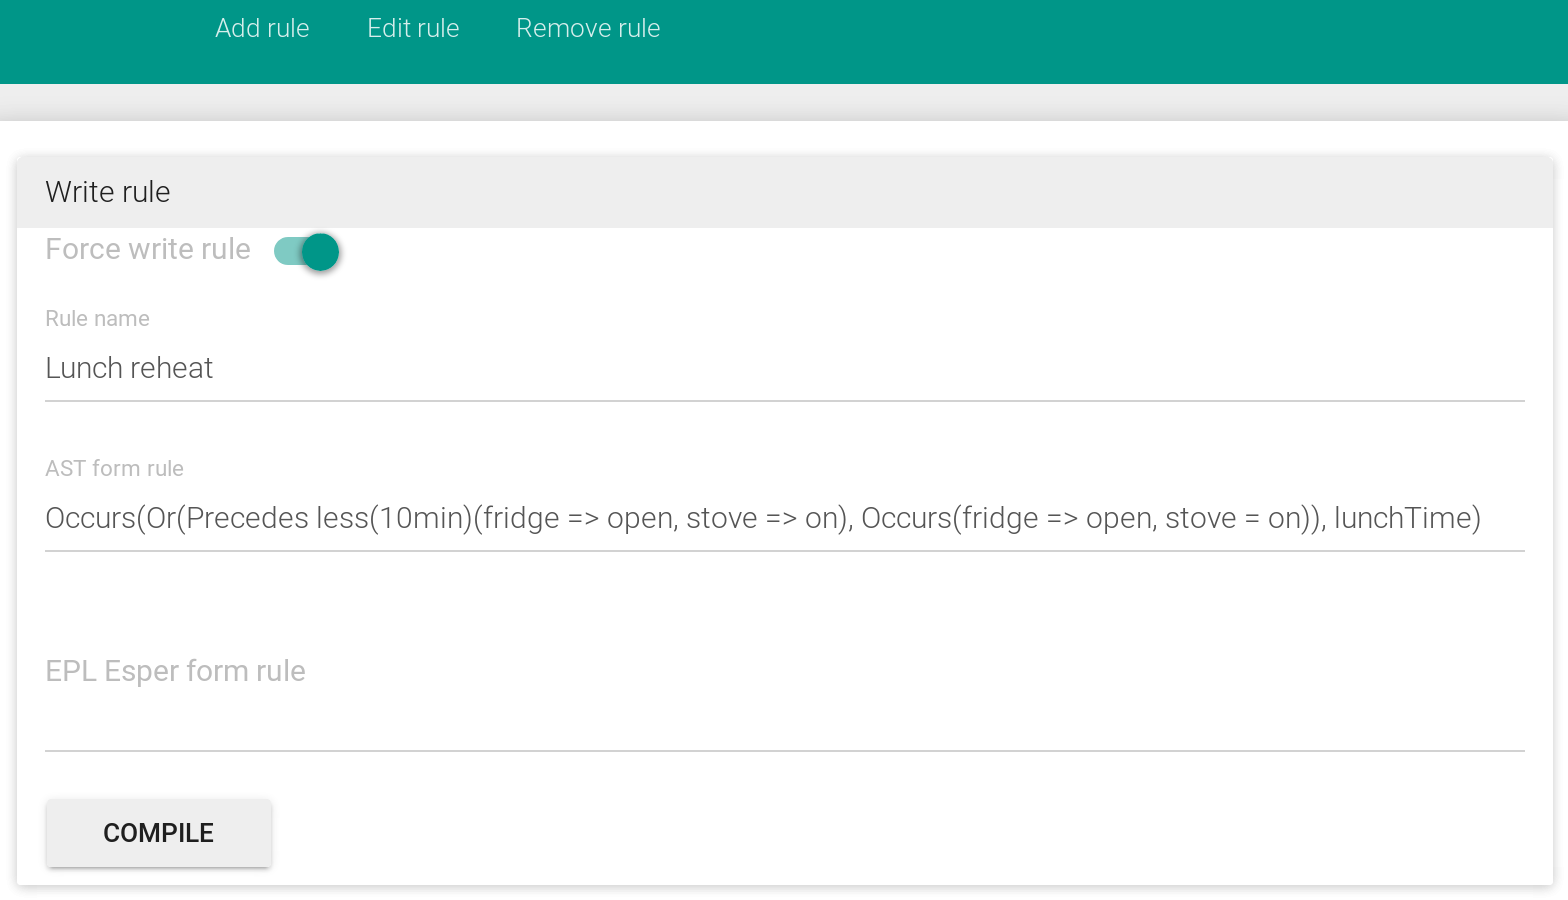
\includegraphics[width=\linewidth,totalheight=\textheight,keepaspectratio]{gfx/ui_add_rule}
\caption{Interface d'administration de service.}
\label{fig:ui_rule}
\end{figure*}

\subsection{Compilation du service}
Les services de haut niveau sont compilés vers un langage de traitement d'évènements qui exprime des règles de plus bas niveau. 
Le langage cible de traitement d'évènements ne supporte pas directement la notion d'état ainsi que nos opérateurs. Lors des étapes de compilation, ces concepts sont donc explicités sous forme de combinaisons d'évènements correspondants.

\subsection{Exécution du service}
Pour être déployées, les règles compilées sont enregistrées auprès du moteur CEP. Notre moteur d'exécution de règle est basé sur Esper, un CEP open-source développé par EsperTech\footnote{\url{http://www.espertech.com/esper/}}. 
Esper propose des interfaces Java et .Net avec NEsper, en tant que bibliothèques pour développer des programmes 
événementiels. Nous avons choisi Esper parce qu'il s'agit d'un moteur CEP 
populaire utilisé à la fois dans l'industrie et dans la recherche. Esper fournit 
un langage spécifique et déclaratif pour le traitement d'évènements complexes, 
appelé EPL (pour Event Processing Language). 
Ce langage inclut tous les opérateurs de SQL, et ajoute des constructions telles que la définition et l'interaction avec des fenêtres, ainsi que pour la génération de sorties.
EPL permet également de décrire des motifs 
d'évènements (ou ``Patterns'' EPL) à identifier dans un flux d'évènements temps réel, en utilisant des 
opérateurs pour ordonner les évènements, des contraintes temporelles, {\em etc.}. Ces opérateurs peuvent s'imbriquer
et permettent de définir explicitement la politique de sélection d'évènements avec la clause ``every''. 
Esper permet de recevoir les données en sorties d'une règle, soit en mode push, par l'utilisation de listeners, soit en mode pull, en utilisant des itérateurs.
%La seconde manière d'exprimer les motifs d'évènements utilise des expressions régulières. 
%Les deux syntaxes offrent la même expressivité.
% Esper propose des interface Java et C\# pour développer des programmes 
% événementiels. Nous avons choisi Esper parce qu'il s'agit d'un moteur CEP 
% populaire utilisé à la fois dans l'industrie et dans la recherche. Esper fournie 
% un langage spécifique et déclaratif pour le traitement d'évènements complexes, 
% appelé EPL (pour Event Processing Language). EPL permet de décrire des motifs 
% d'évènements à identifier dans un flux d'évènements temps réel, en utilisant des 
% opérateurs pour ordonner les évènements, des contraintes temporelles, {\em etc.} 
Cependant, Esper ne permet pas de manipuler le concept d'état, d'où la nécessité
d'encoder cette notion par des motifs purement évènementiels. 

\subsection{Forme canonique}
La forme canonique des données produites par un domicile sensible au contexte 
permet de traiter les mesures d'interaction indépendamment 
de leur format original. Cette forme canonique 
de données, nommée {\em StreamEvent}, est ainsi une couche d'abstraction sur l'hétérogénéité
des évènements des différentes sources, constituant un flux d'évènements uniforme. 
Dans cette représentation, chaque évènement est un 
quadruplet comprenant le type de l'évènement, sa localisation, sa valeur, et l'horodatage de son occurrence.

\[K\] (pour Kinds) est l'ensemble des types d'interactions (\eg Freezer)
\[L\] (pour Locations) est l'ensemble des localisation d'interactions (\eg Kitchen)
\[V\] (pour Values) est l'ensembles des valeurs de chaque domaine d'interaction (\eg open/close)
\[\mathds{N}\] est l'ensemble des horodatages (timestamps) d'instances d'interactions
\[
  v \in \mathds{V} \in \overset{m}{\underset{j=0}\cup}D_{K_i}
\] 
\[ 
t \in \mathds{N}
\]
in
\[
  s \in S=\mathcal{P}(K\times L\times \mathds{V}\times \mathds{N})
\]
\[
  s =\{(k_0,l_0,v^{D_{k_0}}_0,t_0), \dots, (k_n,l_o,v^{D_{k_n}}_n,t_n)\}
\]

Notons que le flux d'évènements en format StreamEvent ainsi défini est plus bas niveau que
le format des rôle défini en Section~\ref{archi:algebra}. En effet, comme dans les langages de CEP, utilisés comme cible,
les évènements sont toujours ponctuels (\ie n'ont pas de durée)\footnote{Même
dans les langages CEP avec une sémantique d'intervalle, les évènements élémentaires
sont toujours ponctuels, comme discuté en Section~\ref{sec:cep}.}, nous ne pouvons pas réutiliser
directement les évènements de rôles, qui étaient estampillés par des intervalles de temps (les périodes).
En revanche, ce nouveau format permet de détecter de manière plus précoce certains évènements
complexes, sans attendre la fin d'un évènement, pouvant avoir une durée non négligeable. Par exemple,
prenons la règle vérifiant si une porte reste ouverte pendant plus de 3 heures. Avec un log
d'évènements de rôles, cette règle ne pouvait déclencher que lorsque la porte était refermée,
car c'est à ce moment-là que l'évènement ``interaction de porte'' se produisait. Au contraire,
avec un log en format StreamEvent, il devient possible d'observer l'ouverture de porte indépendamment
de sa fermeture, et donc de réagir, en principe, dès que le délai de 3 heures s'est écoulé. Nous
verrons par la suite comment notre langage dédié atteint effectivement cette réactivité en
s'appuyant sur le langage cible Esper. Ce niveau de réactivité n'était pas capital dans le contexte
du Chapitre~\ref{cha:fiabilite}, où le signalement à la volée des dysfonctionnements des capteurs 
servait au service de maintenance, ayant un cycle d'intervention de l'ordre de plusieurs jours. Il en
est tout autrement dans le contexte du chapitre actuel où l'on s'intéresse à une classe bien plus large de services,
incluant des assistances de sécurité et des rappels d'activités.


\section{Langage de règles}

Le langage Maloya fournit une base d'expressions contraintes
permettant d'exprimer l'ensemble des services nécessaires à
l'assistance domiciliaire des personnes âgées.  Ce langage permet aux
intervenants de définir des services plus simplement que par des
langages de programmations conventionnels.  En effet, il restreint son
expressivité aux seuls concepts nécessaires au domaine des services
sensibles au contexte pour l'assistance domiciliaire. Pour ce faire,
Maloya rend explicite les notions d'évènements, d'états et les
opérateurs de composition.  

Les intervenants peuvent définir les scénarios correspondant à un
service à travers des règles constituées simplement par des
compositions d'évènements et/ou d'états.  En outre, à cause de la
nature récurrente des services relatifs à l'assistance domiciliaire
(\eg les activités quotidiennes telles que les repas ou la toilette),
une règle est conçue pour que son exécution détecte chaque occurrence
de la composition qu'elle décrit.

Il existe deux représentations du langage~; une représentation interne,
qui constitue la représentation de base de notre langage, et une représentation
textuelle qui permet d'exprimer des règles sous forme d'une phrase en
langage naturel contraint.  Il est important de noter que les
représentations internes et textuelles de notre langage sont
parfaitement équivalentes~: la représentation textuelle étant simplement une
formulation plus naturelle des expressions définies dans la
représentation interne.

\section{Évènements et États}\label{sec:dsl:eventstate}
Notre langage est construit autour de l'expression d'évènements et d'états. 
Un évènement est exprimé ainsi~: 
\begin{lstlisting}[language=MaloyaText]
p becomes v
\end{lstlisting}
% en langage textuel. 
Un état est exprimé comme suit~: 
\begin{lstlisting}[language=MaloyaText]
p is v
\end{lstlisting}
%en langage textuel. 
Dans chaque cas, {\tt p} est l'identification d'une interaction
(matérielle ou logicielle) et {\tt v} appartient à l'ensemble des
valeurs possibles pour l'interaction considérée. L'évènement {\tt p
  {\em becomes} v} survient quand la mesure de l'interaction {\tt p}
signale une valeur {\tt v}, si sa précédente valeur était
différente. L'état {\tt p {\em is} v} commence précisément quand
l'évènement {\tt p {\em becomes} v} se produit~; il se termine quand
l'évènement {\tt p {\em becomes} v'} se produit, où {\tt v'} $\neq$
{\tt v}. Nous voyons la période durant laquelle un état se maintient
comme l'{\em intervalle de temps} d'un état.
%Cette notion est généralisée pour les évènements en les considérant comme des intervalles de temps nuls. 
%NV: a-t-on besoin de considérer un event comme un état de longueur nulle? Je pensais qu'au contraire,
%les opérateurs demandant un état n'acceptent pas un event!

La notion d'intervalle de temps est utilisée pour définir les
opérateurs et leur sémantique. La Figure~\ref{fig:event_state}
présente la syntaxe et la sémantique informelle des évènements et
états.  Un évènement est représenté comme une pointe de signal.
% avec ses points de départs et de fin fusionnés.
Un état est représenté par un signal rectangulaire~; ses points de
départ et de fin correspondent à l'occurrence d'évènements provoquant
son début et sa fin.

\begin{figure}[h]
  \begin{footnotesize}
    % \begin{center}
    \begin{tikzpicture}[node distance=\dx and \dy,
      >=latex,shorten >=2pt,shorten <=2pt,auto,
      semithick,initial distance=1cm,
      every initial by arrow/.style={*->} ]
      \draw[gray!50,line width=0.1mm,dashed] (-1.5,.5) -- (-1.5,-1.2);
      \draw[gray!50,line width=0.1mm,dashed] (1.5,.5) -- (1.5,-1.2);  
      \draw[gray!50,line width=0.1mm,dashed] (-.5,.2) -- (-.5,-1.);
      \draw[gray!50,line width=0.1mm,dashed] (.5,.2) -- (.5,-1.);  
      \draw[] (-1.5,.) 
      node[xshift=-3 cm,yshift=.125cm] { Event~:} 
      node[xshift=-1.5 cm,yshift=.3cm] { {\tt p {\em becomes} v}} 
      node[xshift=-1.5 cm,yshift=. cm] { $p\Rightarrow v$} 
      node[xshift=-.2 cm,yshift=0 cm] { {\tt e}} --(-.5,.)--(-.5,.4) -- (-.5,.) -- (1.5,.);
      \draw[] (-1.5,-.6) 
      node[xshift=-.12 cm,yshift=.25cm] { ${\tt v}$} 
      node[xshift=-.1 cm,yshift=. cm] { ${\tt v'}$} 
      node[xshift=-.25 cm,yshift=.125 cm] { {\tt p}} -- (-.5,-.6) -- (-.5,-.2) -- (.5,-.2) -- (.5,-.6) -- (1.5,-.6);
      \draw[] (-1.5,-1.2) 
      node[xshift=-3 cm,yshift=.125cm] { State~:} 
      node[xshift=-1.5 cm,yshift=.3cm] { {\tt p {\em is} v}} 
      node[xshift=-1.5 cm,yshift=. cm] { $p=v$} 
      node[xshift=-.2 cm,yshift=0 cm] { {\tt s}} -- (-.5,-1.2) -- (-.5,-.8) -- (.5,-.8) -- (.5,-1.2) -- (1.5,-1.2);
    \end{tikzpicture}
  \end{footnotesize}
  \caption{Semantique informelle et syntaxe des état et évènement.}
  \label{fig:event_state}
\end{figure}

Les états disposent également de filtres sur leur durée.  Ces filtres
permettent de borner la période d'un état avec une limite haute ou une
limite basse. La limite haute de la durée d'un état est exprimée
ainsi~:
\begin{lstlisting}[language=MaloyaText]
p is v less than t
\end{lstlisting}
et la limite basse est exprimée comme suit~:
\begin{lstlisting}[language=MaloyaText]
p is v for at least t
\end{lstlisting}
où {\tt t} représente une période de temps.

\section{Les opérateurs}\label{sec:dsl:operator}
Une {\em règle} dans notre langage est constituée d'opérateurs manipulant les 
états et/ou les évènements. Tous les opérateurs retournent des évènements.
Plus précisément, un opérateur produit un évènement de succès quand le contexte 
décrit par l'application de l'opérateur à des états/évènements est détecté.
Puisqu'un opérateur retourne un évènement, les opérateurs qui prennent en argument un évènement
peuvent prendre également une application d'opérateur comme argument.
En revanche, les opérateurs qui prennent un état comme argument ne peuvent 
pas prendre une application d'opérateur comme argument.
L'imbrication des opérateurs n'est ainsi pas arbitraire et suit notre étude de domaine.

La Figure~\ref{fig:operators} présente la double syntaxe des
opérateurs de notre langage (représentation interne et textuelle),
ainsi que sa sémantique informelle.  La syntaxe est présentée sur la
partie gauche. Sur la partie droite, une représentation graphique,
suggère la sémantique de l'opérateur comme une fonction booléene
définie sur le temps.  Cette représentation permet de visualiser les
évènements et les états impliqués dans une application d'opérateur, et
la façon dont les opérateurs les combinent.
%Chaque construction en langage textuelle est complétée de sa construction équivalente en langage c\oe ur.
% example greater less
%variant : precedes less, precedes greater

%\end{center}
 % \begin{multicols}{2}
\begin{figure*}[!h]
\begin{footnotesize}
\begin{tikzpicture}[node distance=\dx and \dy,
      >=latex,shorten >=2pt,shorten <=2pt,auto,
      semithick,initial distance=1cm,
      every initial by arrow/.style={*->} ]   
      \draw[gray!50,line width=0.1mm,dashed] (-1.5,.5) -- (-1.5,-1.2);
      \draw[gray!50,line width=0.1mm,dashed] (1.5,.5) -- (1.5,-1.2);  
      %%%%%%%%%%%%%%%%%%%%%%%%%%%%%%%%%%%%%%%%%%%%%%%%%%%%%%%%%%%%%%%%%%%%%%%
      \draw[gray!50,line width=0.1mm,dashed] (.5,.) -- (.5,-1.2);   
      \draw[] (-1.5,.) 
      node[xshift=-.25 cm,yshift=.125cm] {{\tt e$_1$}}  --(-.5,.)--(-.5,.4) -- (-.5,.) -- (1.5,.);
      \draw[] (-1.5,-.6) 
      node[xshift=-.25 cm,yshift=.125cm] {{\tt e$_2$}} -- (.5,-.6) -- (.5,-.2) -- (.5,-.6) -- (1.5,-.6);
      \draw[] (-1.5,-1.2) 
      node[xshift=-4.1 cm,yshift=1.cm] {Every time {\tt e$_1$} {\em immediately} precedes {\tt e$_2$}}
      node[xshift=-3. cm,yshift=.25cm] {{\tt e$_1$ {\bf precedes} e$_2$ $\Leftrightarrow$ $Precedes(e_1,e_2)$}}
      node[xshift=-1.5 cm,yshift=-.45cm] {Variants:}
      node[xshift=3.5 cm,yshift=-.3cm] {{\tt e$_1$ {\bf precedes within} t e$_2$ $\Leftrightarrow$ $Precedes\_less(t)(e_1,e_2)$}}
      node[xshift=3.45 cm,yshift=-.65cm] {{\tt e$_1$ {\bf precedes by} t e$_2$ $\Leftrightarrow$ $Precedes\_greater(t)(e_1,e_2)$}} -- (.5,-1.2) -- (.5,-.8) -- (.5,-1.2) -- (1.5,-1.2);
      %%%%%%%%%%%%%%%%%%%%%%%%%%%%%%%%%%%%%%%%%%%%%%%%%%%%%%%%% 
      \draw[gray!50,line width=0.1mm,dashed] (-1.5,-2.) -- (-1.5,-3.7);
      \draw[gray!50,line width=0.1mm,dashed] (1.5,-2.) -- (1.5,-3.7);  
      \draw[gray!50,line width=0.1mm,dashed] (-.5,-2.5) -- (-.5,-3.7);   
      \draw[gray!50,line width=0.1mm,dashed] (.,-2.5) -- (.,-3.7);  
      \draw[gray!50,line width=0.1mm,dashed] (.5,-2.5) -- (.5,-3.7);
      \draw[] (-1.5,-2.5) 
      node[xshift=-.25 cm,yshift=.125cm] {{\tt e}} --(-.5,-2.5)--(-.5,-2.1)--(-.5,-2.5)--(.,-2.5)--(.,-2.1)--(.,-2.5)--(.5,-2.5)--(.5,-2.1)--(.5,-2.5) -- (1.5,-2.5);
      \draw[] (-1.5,-3.1) 
      node[xshift=-.25 cm,yshift=.125cm] {{\tt s}} -- (-1,-3.1) -- (-1,-2.7) -- (1,-2.7) -- (1,-3.1) -- (1.5,-3.1);
      \draw[] (-1.5,-3.7) 
      node[xshift=-4.35 cm,yshift=1.cm] {Every time {\tt e} occurs during state {\tt s}}
      node[xshift=-3. cm,yshift=.125cm] {{\tt e {\bf during} s $\Leftrightarrow$ $During(e,s)$}}  -- (-.5,-3.7) -- (-.5,-3.3)--(-.5,-3.7)--(.,-3.7)--(.,-3.3)--(.,-3.7)--(.5,-3.7)--(.5,-3.3)--(.5,-3.7) -- (1.5,-3.7);
      %%%%%%%%%%%%%%%%%%%%%%%%%%%%%%%%%%%%%%%%%%%%%%%%%%%%%%%%%%%%%%%%%%%%%%% 
      \draw[gray!50,line width=0.1mm,dashed] (-1.5,-4.6) -- (-1.5,-6.2);
      \draw[gray!50,line width=0.1mm,dashed] (1.5,-4.6) -- (1.5,-6.2);
      \draw[gray!50,line width=0.1mm,dashed] (.5,-5.) -- (.5,-6.2);
      \draw[] (-1.5,-5) 
      node[xshift=-.25 cm,yshift=.125cm] {{\tt s$_1$}} -- (-1,-5) -- (-1,-4.6) -- (.5,-4.6) -- (.5,-5) -- (1.5,-5);
      \draw[] (-1.5,-5.6) 
      node[xshift=-.25 cm,yshift=.125cm] {{\tt s$_2$}} -- (-.5,-5.6) -- (-.5,-5.2) -- (1,-5.2) -- (1,-5.6) -- (1.5,-5.6);
      \draw[] (-1.5,-6.2) 
      node[xshift=-3.9 cm,yshift=1.cm] {Every time state {\tt s$_1$} overlaps with state {\tt s$_2$}}
      node[xshift=-3. cm,yshift=.25cm] {{\tt s$_1$ {\bf overlapping} s$_2$ $\Leftrightarrow$ $Overlapping(s_1,s_2)$}} 
      node[xshift=-1.5 cm,yshift=-.45cm] {Variants:}
      node[xshift=4.10 cm,yshift=-.3cm] {{\tt s$_1$ {\bf overlapping} {\bf within} t s$_2$ $\Leftrightarrow$ $Overlapping\_less(t)(s_1,s_2)$}}
      node[xshift=4.05 cm,yshift=-.65cm] {{\tt s$_1$ {\bf overlapping} {\bf for} t s$_2$ $\Leftrightarrow$ $Overlapping\_greater(t)(s_1,s_2)$}} -- (-.5,-6.2) -- (.5,-6.2) -- (.5,-5.8) -- (.5,-6.2) -- (1.5,-6.2);
      %%%%%%%%%%%%%%%%%%%%%%%%%%%%%%%%%%%%%%%%%%%%%%%%%%%%%%%%%%%%%%%%%%%%%%%
      \draw[gray!50,line width=0.1mm,dashed] (-1.5,-7.1) -- (-1.5,-8.7);
      \draw[gray!50,line width=0.1mm,dashed] (1.5,-7.1) -- (1.5,-8.7);
      \draw[gray!50,line width=0.1mm,dashed] (-.5,-7.1) -- (-.5,-8.7);
      \draw[] (-1.5,-7.5) 
      node[xshift=-.25 cm,yshift=.125cm] {{\tt e}} --(-.5,-7.5)--(-.5,-7.1)--(-.5,-7.5)--(.,-7.5)--(.,-7.1)--(.,-7.5)--(.5,-7.5)--(.5,-7.1)--(.5,-7.5) -- (1.5,-7.5);
      \draw[] (-1.5,-8.1) 
      node[xshift=-.25 cm,yshift=.125cm] {{\tt s}} -- (-1.,-8.1) -- (-1.,-7.7) -- (1.,-7.7) -- (1,-8.1) -- (1.5,-8.1);
      \draw[] (-1.5,-8.7) 
      node[xshift=-3.7 cm,yshift=1.cm] {The first occurrence of event {\tt e} during state {\tt s}}
      node[xshift=-3 cm,yshift=.125cm] {{\tt e {\bf occurs while} s $\Leftrightarrow$ $Occurs(e,s)$}} -- (-.5,-8.7) -- (-.5,-8.3) -- (-.5,-8.7) -- (1.5,-8.7);
      % %%%%%%%%%%%%%%%%%%%%%%%%%%%%%%%%%%%%%%%%%%%%%%%%%%%%%%%%%%%%%%%%%%%%%%% 
      \draw[gray!50,line width=0.1mm,dashed] (-1.5,-9.6) -- (-1.5,-11.2);
      \draw[gray!50,line width=0.1mm,dashed] (1.5,-9.6) -- (1.5,-11.2);  
      \draw[gray!50,line width=0.1mm,dashed] (-.5,-9.6) -- (-.5,-11.2);  
      \draw[line width=0.1mm,dashed](-1.,-9.6)--(1,-9.6) ; 
      \draw[]  (-.5,-9.6) 
      node[xshift=-1.25 cm,yshift=-.25cm] {{\tt s$_1$}}  -- (.,-9.6); 
      \draw[] (-1.5,-10.6) 
      node[xshift=-.25 cm,yshift=.125cm] {{\tt s$_2$}} -- (-1,-10.6) -- (-1,-10.2) -- (1,-10.2) -- (1,-10.6) -- (1.5,-10.6);
      \draw[] (-1.5,-11.2) 
      node[xshift=-4.6 cm,yshift=1.3cm] {The first occurrence of state {\tt s$_1$}}
      node[xshift=-3. cm,yshift=1.cm] {(partially) superposed with state {\tt s$_2$}}
      node[xshift=-3.2 cm,yshift=.25cm] {{\tt s$_1$ {\bf occurs while} s$_2$ $\Leftrightarrow$ $Occurs(${\tt s$_1$},{\tt s$_2$}$)$}}
      node[xshift=-1.5 cm,yshift=-.45cm] {Variants:}
      node[xshift=3.8 cm,yshift=-.3cm] {{\tt s$_1$ {\bf occurs within} t {\bf while} s$_2$ $\Leftrightarrow$ $Occurs\_less(t)(s_1,s_1)$}}
      node[xshift=3.75 cm,yshift=-.65cm] {{\tt s$_1$ {\bf occurs for} t {\bf while} s$_2$ $\Leftrightarrow$ $Occurs\_greater(t)(s_1,s_1)$}}  -- (-.5,-11.2) -- (-.5,-10.8) -- (-.5,-11.2) -- (1.5,-11.2) ;
      % %%%%%%%%%%%%%%%%%%%%%%%%%%%%%%%%%%%%%%%%%%%%%%%%%%%%%%%%%%%%%%%%%%%%%%%
      \draw[gray!50,line width=0.1mm,dashed] (-1.5,-12.1) -- (-1.5,-15);
      \draw[gray!50,line width=0.1mm,dashed] (1.5,-12.1) -- (1.5,-15);  
      \draw[gray!50,line width=0.1mm,dashed] (-.5,-13.1) -- (-.5,-14);  
      \draw[gray!50,line width=0.1mm,dashed] (.5,-12.1) -- (.5,-15); 
      
      \draw[] (-1.5,-12.5) 
      node[xshift=-.25 cm,yshift=.125cm] {{\tt e$_1$}} -- (.5,-12.5)--(.5,-12.1)--(.5,-12.5)--(1.5,-12.5);
      \draw[] (-1.5,-13.1) 
      node[xshift=-.25 cm,yshift=.125cm] {{\tt e$_n$}} -- (-.5,-13.1) -- (-.5,-12.7) -- (-.5,-13.1) -- (1.5,-13.1);

      % \draw[gray!50,line width=0.1mm,dashed] (-1.5,-5.6) -- (-1.5,-6.);
      % \draw[gray!50,line width=0.1mm,dashed] (1.5,-5.6) -- (1.5,-6.);  
      \draw[] (-1.5,-14.) 
      node[xshift=-3.7 cm,yshift=.5cm] {Trigger whenever any of the events happens}
      node[xshift=-3. cm,yshift=.125cm] {{\tt {\bf \{}e$_1$ {\bf or} $\dots$ {\bf or} e$_n${\bf\}} $\Leftrightarrow$ $Or(e_1,\dots , e_n)$ }} -- (-.5,-14.) -- (-.5,-13.6) -- (-.5,-14.) -- (.5,-14.) -- (.5,-13.6) -- (.5,-14.) -- (1.5,-14.);
      % %%%%%%%%%%%%%%%%%%%%%%%%%%%%%%%%%%%%%%%%%%%%%%%%%%%%%%%%%%%%%%%%%%%%%%% 
      % \draw[gray!50,line width=0.1mm,dashed] (-1.5,-6.6) -- (-1.5,-7.);
      % \draw[gray!50,line width=0.1mm,dashed] (1.5,-6.6) -- (1.5,-7.);  
      \draw[] (-1.5,-15) 
      node[xshift=-4. cm,yshift=.5cm] {Trigger as soon as every event happens}
      node[xshift=-3. cm,yshift=.125cm] {{\tt {\bf\{}e$_1$ {\bf and} $\dots$ {\bf and} e$_n${\bf\}} $\Leftrightarrow$ $And(e_1,\dots , e_n)$ }} -- (.5,-15) -- (.5,-14.6) -- (.5,-15) -- (1.5,-15);
      %%%%%%%%%%%%%%%%%%%%%%%%%%%%%%%%%%%%%%%%%%%%%%%%%%%%%%%%%%%%%%%%%%%%%%% 
    \end{tikzpicture}
%  \end{multicols}
  \caption{Sémantique informelle et syntaxe des opérateurs du langage Maloya.}
  \label{fig:operators}
  \end{footnotesize}
\end{figure*} 
Les opérateurs définis dans le langage, listés dans la Figure~\ref{fig:operators}, 
correspondent à des opérateurs de l'algèbre d'Allen sur les intervalles de temps~\paulcite{allen1983maintaining}.
% , 
% si on considère les états et les évènements en tant qu'intervalles de temps, 
% comme expliqué précédemment. 

Cependant, 
% NV: On ne peut pas faire la discussion en général car Precedes est le seul opérateur ou on
% n'admet que les occurrences les plus proches; pour During par exemple, on les prend toutes, au contraire, non?
%les opérateurs d'Allen modélisent toutes les relations possibles 
%entre deux intervalles de temps, telles que la relation de {\em précédence}, 
%un intervalle qui arrive {\em durant} un autre, ou un intervalle qui en 
%{\em chevauche} un autre, et ce, pour toutes leurs occurrences. Par exemple 
l'opérateur de l'algèbre d'Allen
\begin{lstlisting}
X before Y
\end{lstlisting}
reconnaît toutes les occurrences de {\tt X} qui précèdent toutes les
occurrences de {\tt Y}. Par exemple, dans la série d'intervalle
suivante~:
\begin{small}
\begin{Verbatim}[fontsize=\small] 
XXX YY
\end{Verbatim}
\end{small}
il identifie 6 paires (X,Y) correspondant à toutes les combinaisons
des occurrences.  Dans le cadre de la sensibilité au contexte pour
l'assistance domiciliaire, il n'est pas nécessaire d'identifier
plusieurs combinaisons des occurrences des évènements X et Y. Par
exemple, si il y a eu une détection d'ouverture du frigidaire, suivie
d'une détection de l'utilisation du four, il est inutile de prendre en
considération les autre occurrences d'ouverture du frigidaire qui
précèdent, ni les utilisations suivantes du four.  Pour cette raison,
notre opérateur Precedes prend en compte seulement la dernière
occurrences de l'évènement X (ouverture du frigidaire dans l'exemple)
immédiatement suivie par la première occurrence de l'évènement Y
(utilisation du four dans l'exemple).
% NV: je ne comprends pas cette notation:
%Par conséquent, le résultat obtenu serait:
%\begin{small}
%\begin{Verbatim}[fontsize=\small]
%X Y
%\end{Verbatim}
%\end{small}
% NV: what else? (que Precedes)
%Ainsi, certains de nos opérateurs contraignent leurs opérandes à une seule occurrence reconnue.

% NV: Je pense que dans tout CEP, les évènements d'un même type se cheauchant ont 
% des attributs différents. Mais alors nous aussi on a des events de Presence qui se chevauchent,
% correspondant à des pièces différentes, non?

%De plus, le flux d'évènements du domicile est séquentiel dans le sens où il ne 
%peut pas y avoir plusieurs occurrences d'un même interaction qui se chevauchent, 
%limitant ainsi le besoin d'expressivité de nos opérateurs. Par exemple, l'opérateur d'Allen
%\begin{lstlisting}
%X during Y
%\end{lstlisting}
%Autorise la reconnaissance de la série d'intervalle suivante:
%\begin{small}
%\begin{Verbatim}[fontsize=\small]
% X X X X X
%YYYYYY
%   YYYYYYYY
%\end{Verbatim}
%\end{small}
%Dans notre domaine il ne peut pas il avoir de chevauchement d'occurrences de {\tt Y}. 

Nous avons ainsi généralisé les opérateurs d'Allen entre deux
intervalles pour prendre en compte les multiples occurrences de ces
intervalles. De plus, les opérateurs d'Allen n'acceptent que des
intervalles non vides~; nous les avons donc généralisés, lorsque
nécessaire, pour accepter aussi des évènements.  En outre, pour
certains opérateurs, nous avons défini une variante prenant en compte
une contrainte temporelle, introduisant une limite basse et une limite
haute pour la durée de la composition des opérandes.

Dans la suite du chapitre, par convention, les évènements
%{\tt p {\em becomes} v} 
seront notés avec la lettre {\tt e} (possiblement indicée), et les états 
%{\tt p {\em is} v} 
seront notées avec la lettre {\tt s} (possiblement indicée).

\subsection{Precedes}
Cet opérateur rapporte un succès lorsqu'une occurrence de l'évènement 
{\tt e$_1$} précède {\em immédiatement} une occurrence de l'évènement {\tt e$_2$}. 
Il ne doit pas y avoir d'autres occurrence des évènements {\tt e$_1$} ou 
{\tt e$_2$} entre les occurrences identifiées. 
\begin{lstlisting}[language=MaloyaText]
e$_1$ precedes e$_2$
\end{lstlisting}
Pour couvrir les scénarios d'assistance dans notre domaine cible, nous
devons étendre l'expressivité de cet opérateur, avec des contraintes
temporelles optionnelles. Plus précisément, nous introduisons deux
variantes de cet opérateur~:
\begin{lstlisting}[language=MaloyaText]
e$_1$ precedes within t e$_2$
e$_1$ precedes by t e$_2$
\end{lstlisting}
La contrainte temporelle est définie par le paramètre {\tt t}. Ces
variantes définissent les limites hautes et basses des durées entre
les occurrences des opérandes évènements.

\subsection{During}
Cet opérateur réussit chaque fois que l'évènement {\tt e} se produit
durant l'état {\tt s}.
\begin{lstlisting}[language=MaloyaText]
e during s
\end{lstlisting}
Il n'y a pas de versions de cet opérateur avec des contraintes
temporelles.

\subsection{Overlapping}
Cet opérateur réussit quand une occurrence de l'état {\tt s$_1$} chevauche 
une occurrence suivante de l'état
%l'occurrence {\em immédiatement} suivante de l'état 
{\tt s$_2$}. L'état {\tt s$_1$} commence avant le début de l'état 
{\tt s$_2$}, et se termine durant {\tt s$_2$}, comme montré en 
Figure~\ref{fig:operators}. 
\begin{lstlisting}[language=MaloyaText]
s$_1$ overlapping s$_2$
\end{lstlisting}
%\clearpage

Les versions avec contraintes temporelles définissent les limites
hautes et basses de la durée de chevauchement des occurrences de ces
états. Ces versions sont notées comme suit~:
\begin{lstlisting}[language=MaloyaText]
s$_1$ overlapping within t s$_2$
s$_1$ overlapping for t s$_2$
\end{lstlisting}

\subsection{Occurs while}
Cet opérateur est similaire à l'opérateur {\tt during}, mais réussit
{\em uniquement} pour la première occurrence de l'évènement {\tt e} qui se 
produit durant l'état {\tt s}.
\begin{lstlisting}[language=MaloyaText]
e occurs while s
\end{lstlisting} 
Une variante de cette règle est 
\begin{lstlisting}[language=MaloyaText]
s$_1$ occurs while s$_2$
\end{lstlisting}
Dans ce cas, l'opérateur réussit la première fois que l'état {\tt
  s$_1$} se superpose au moins partiellement avec {\tt s$_2$}. Les
versions avec contraintes temporelles de cet opérateur donnent les
limites hautes et basses pour la durée de superposition des
états. Elles sont notées comme suit~:
\begin{lstlisting}[language=MaloyaText]
s$_1$ occurs within t while s$_2$
s$_1$ occurs for t while s$_2$
\end{lstlisting}


%En langage coeur les contraintes temporelles sont exprimés avec les marqueurs $greater(t)$ ou $less(t)$ ajouté aux opérateur à dériver.

Bien que les opérateurs d'Allen expriment un large éventail de
situations, ils ne couvrent pas tous les besoins révélés par notre
analyse de domaine. De nouveaux opérateurs doivent être introduits. 

\subsection{Or}
En
particulier, une disjonction d'événements est nécessaire pour
permettre l'expression de contextes alternatifs. Une règle disjonctive
est de la forme~:
\begin{lstlisting}[language=MaloyaText]
{ e$_1$ or $\dots$ or e$_n$ }
\end{lstlisting}
%{\tt \{e$_1$ {\bf or} \ldots~{\bf or} e$_n$\}}; 
Elle réussit quand le premier des évènements {\tt e$_i$} se produit dans le flux. 

\subsection{And}
Nous introduisons également une règle de conjonction de la forme~: 
\begin{lstlisting}[language=MaloyaText]
{ e$_1$ and $\dots$ and e$_n$ }
\end{lstlisting}
%{\tt \{e$_1$ {\bf and} \ldots~{\bf and} e$_n$\}}. 
Cette règle réussit une fois que chacun des évènements {\tt e$_i$} s'est produit au moins une fois.

\section{Les opérandes}
Comme expliqué précédemment, les opérandes sont soit des états, soit des évènements. Si les opérandes ne sont pas des compositions de règles (possible si l'opérande requise par l'opérateur est un évènement), ils sont alors l'expression des mesures d'interactions de l'utilisateur avec son environnement. Dans ce cas ils sont exprimé de façon à correspondre aux besoins du domaine, et plus particulièrement d'une installation.

Les interactions sont décrites dans une tables statique. Cette table définit les attributs de chaque interaction dans un domicile donné, comme illustré en Figure~\ref{listing:table_static_generique}.

\begin{figure}
\begin{lstlisting}[frame=bt]
"name":{
  "location":"location",
  "kind":"kind",
  "values":["val1","val2"]
}
\end{lstlisting}
\caption{Table statique générique.}
\label{listing:table_static_generique}
\end{figure}

Cette table décrit le nom de l'interaction (\eg freezer), sa localisation (\eg kitchen), son type (\eg Freezer), et ses valeurs possibles (\eg open/close). Cependant, certaines interactions, principalement les interactions de présence, n'ont pas de localisation spécifiée dans cette table. En effet, ces interactions, étant possibles à de multiples endroits dans le domicile, sa localisation doit être précisée lors de son instanciation dans la règle entre parenthèse (\eg {\it Presence(Kitchen)}). De plus, il est possible de vouloir définir un opérande qui concerne toutes les interactions, par exemple pour définir une règle qui identifie les problèmes de communication de tout capteur. Pour ce faire nous avons introduit le mot clé {\em ``Any''}~:
\begin{lstlisting}[language=MaloyaText]
Commfailure( Any ) becomes true
\end{lstlisting}

\section{Exprimer un service}
Nous illustrons maintenant l'utilisation de nos opérateurs en écrivant la règle 
en Maloya pour l'activité ``Lunch Reheat'', décrite précédemment (Section~\ref{domain:scenario}). 
%It is used as a running example throughout this section to further introduce our DSL and its implementation.
\begin{figure}[h]
\begin{lstlisting}[language=MaloyaText,frame=bt]
{ ( freezer becomes open precedes 
    within 10 minutes stove becomes on )
  or
  ( freezer becomes open occurs while stove is on ) 
} occurs while lunchTime
\end{lstlisting}
\caption{Code Maloya textuel pour le service ``Lunch Reheat''.}
\label{listing:maloyaText_reheat}
\end{figure}

Notons que cette spécification encode deux variantes d'un scénario~: (1) prendre 
un repas depuis le frigidaire, ensuite allumer le four dans les 10 minutes qui suivent~; (2) prendre un repas 
depuis le frigidaire pour le mettre dans le four, qui est déjà allumé. Le tout durant la période du déjeuner.

% Notons également que les éléments de la règle décrivant les interactions comme 
% {\em freezer} et leurs états possibles, doivent être décrits dans une table 
% statique, dont un exemple est donné en Figure~\ref{listing:table_static_freezer}. 
% Cette table définie les attributs de chaque interaction dans un domicile donné.
% \begin{figure}[h!]
% %\begin{footnotesize}
% \begin{lstlisting}[frame=bt]
% "freezer":{
% 	"location": "Kitchen",
% 	"kind": "Freezer",
% 	"values": ["open", "close"]
% }
% \end{lstlisting}
% \caption{Exemple de table statique pour l'interaction freezer.}
% \label{listing:table_static_freezer}
% %\end{footnotesize}
% \end{figure}

\section{Étapes de compilation}\label{dsl:compilation}
La compilation est faite en trois étape. La règle en langage textuel est 
compilée vers le langage interne, qui sont équivalents. La règle en 
langage interne est ensuite compilée vers une représentation intermédiaire qui est un 
pseudo-code EPL. Ce dernier est finalement compilé vers sa représentation finale en EPL.
\clearpage
\subsection{Représentation interne}
La première étape consiste à retranscrire le texte de la règle en langage dédié vers 
la représentation interne du langage Maloya~; cette traduction est définie par une correspondance biunivoque.
Par exemple, dans le langage interne, la représentation de l'opérateur {\tt e {\bf during} s} devient $During(e,s)$. 
Ainsi, la traduction de notre exemple vers le langage interne de Maloya correspond à ce qui suit.
\begin{figure}[!h]
\begin{lstlisting}[language=Maloya]
  Occurs(Or(
          Precedes_less(10min)(freezer => open, stove => on),
          Occurs(freezer => open, stove = on)),
       lunchTime)
\end{lstlisting}
\caption{Code Maloya interne pour le service ``Lunch Reheat''.}
\label{listing:maloya_reheat}
\end{figure}

\noindent
où ``{\em =$>$}'' désigne un évènement qui se produit et ``{\em =}'' désigne un 
état qui se maintient.
% et auquel on souhaite accéder.

\subsection{Pseudo-code EPL}
L'étape de compilation suivante génère du pseudo-code EPL. Ce pseudo-code 
utilise seulement les opérateurs EPL, mais n'instancie pas les attributs des 
évènements~; cette instanciation est faite ultérieurement. Cette étape implique 
plusieurs transformations. Premièrement, comme EPL n'offre pas la notion d'état, 
chaque état dans une règle est traduit par une séquence correspondant aux 
évènements qui marquent le début et la fin de l'état, ordonnée avec des opérateurs 
EPL standards. De cette façon, l'état exprimant le four comme étant allumé est 
traduit en une séquence EPL correspondant au four devenant allumé, suivi par 
n'importe quel évènement d'intérêt mais sans que le four n'ait été éteint. 
Par conséquent, l'opérateur ``{\em Occurs(\dots, stove = on)}'' est traduit en EPL par 
%\begin{quote} {\em stove $=>$ on $\rightarrow$ \dots\ and\ not\ (stove $=>$ off)} \end{quote}
\begin{lstlisting}[language=EPLPseudoCode,frame=none]
stove => on -> $\dots$ and not stove => off
\end{lstlisting}
\noindent 
utilisant les opérateurs EPL ``{\em and}'', ``{\em not}'' et ``->'', 
qui correspond à {\em followed by} (suivi de la première occurrence de). De plus, 
dans cette phase de compilation, les contraintes temporelles sont traduites par 
l'utilisation explicite de la construction EPL ``{\tt $where$ $timer$:$within$}'' pour 
exprimer la limite haute, et l'utilisation explicite de ``{\tt $and$ $timer$:$interval$}'' 
pour exprimer la limite temporelle basse. 



Par défaut, EPL limite la reconnaissance d'un évènement à une seule occurrence. 
Cette étape introduit donc la construction EPL ``{\em every}'', 
%Cette étape introduit donc les constructions EPL ``{\em every}'' et ``{\em every-distinct}'', 
pour (1) gérer les occurrences d'un évènement en fonction de l'expressivité requise 
par l'opérateur, et (2) pour gérer la nature récurrente des règles en elles-mêmes.

La composition d'opérateurs peut nécessiter la construction d'une fenêtre (``{\em window}''). 
L'opérateur utilisé comme opérande est alors compilé séparément et l'évènement produit est capturé dans une
fenêtre nouvellement créée. 
L'opérateur composé peut alors utiliser cet évènement de la même manière qu'un évènement élémentaire,
à travers l'identifiant de la fenêtre.

En poursuivant notre exemple, le résultat de 
cette phase de compilation en pseudo-code EPL est~:
\begin{figure}[!h]
\begin{lstlisting}[language=EPLPseudoCode]
//Window1:
( every freezer => open -> 
    stove => on 
    and not ( freezer => open ) where timer:within(10min) ) 
or  
( every stove => on -> 
    freezer => open 
    and not ( stove => off ) ) 

//Main rule:
every lunchTime => begin ->
  Window1( timestamp > (lunchTime => begin).timestamp )
  and not ( lunchTime => end )
\end{lstlisting}
\caption{Pseudo-code EPL pour le service ``Lunch Reheat''.}
\label{listing:pseudo_reheat}
\end{figure}

\subsection{EPL Esper}
L'étape finale consiste à obtenir la représentation EPL Esper, depuis le pseudo-code EPL, 
en effectuant l'instanciation des attributs nécessaires dans le flux d'événements 
canoniques ({\em i.e.,} la forme StreamEvent) en utilisant la table
statique mentionnée précédemment.

De plus, cette étape lie dans la formule EPL tous les évènements comme provenant d'un même domicile 
(avec la contrainte EPL ``{\tt user=$X$.user}''). 

Les résultats de ces transformations nous permettent d'obtenir la représentation finale de la 
règle en EPL Esper qui est exécutée par le moteur Esper~:
\clearpage
\begin{figure}[h!]
\begin{lstlisting}[language=EPL]
create window Wind.std:unique(location,kind,user) 
select * from StreamEvent

insert into Wind select arg from pattern [ 
  (every arg=StreamEvent( location='Kitchen',kind='Freezer',
                          status='open' ) ->
     StreamEvent( location='Kitchen',kind='Stove',
                  status='on',user=arg.user ) 
     and not ( StreamEvent( location='Kitchen',kind='Freezer',
                            status='open',user=arg.user )) 
     where timer:within (10min) )
  or ( every arg=StreamEvent( location='Kitchen',kind='Stove',
                              status='on' ) -> 
         StreamEvent( location='Kitchen',kind='Freezer',
                      status='open',user=arg.user ) 
         and not StreamEvent( location='Kitchen',kind='Stove',
                              status='off',user=arg.user )) 
]

select Cal_L_b,arg from pattern [ 
  every Cal_L_b= StreamEvent( location='Lunch',kind='Calendar',
                              status!='end') ->
    arg=Wind(timestamp>Cal_L_b.timestamp,
             user=Cal_L_b.user) 
    and not StreamEvent( location='Lunch',kind='Calendar',
                         status='end',user=Cal_L_b.user )) 
]
\end{lstlisting}
\caption{Code EPL compilé final pour le service ``Lunch Reheat''.} 
\label{listing:epl_reheat}
\end{figure}

% \begin{figure}[h!]
% \begin{lstlisting}[language=EPL]
% select Cal_L_b,Fre_K_o,Sto_K_o from pattern [ 
%   every Cal_L_b=StreamEvent(role.location='Lunch',
%                             role.kind='Calendar',
%                             status!='end') -> 
%     every-distinct(location,kind)
%     ((every
%       Fre_K_o=StreamEvent(role.location='Kitchen',
%                           role.kind='Freezer',
%                           status='open',
%                           user=Cal_L_b.user) -> 
%         Sto_K_o=StreamEvent(role.location='Kitchen',
%                             role.kind='Stove',
%                             status='on',
%                             user=Cal_L_b.user) 
%         where timer:within(10min)
%         and not (StreamEvent(role.location='Kitchen',
%                              role.kind='Freezer',
%                              status='open',
%                              user=Cal_L_b.user))) 
%    or(every
%       Sto_K_o=StreamEvent(role.location='Kitchen',
%                           role.kind='Stove',
%                           status='on', 
%                           user=Cal_L_b.user) -> 
%       every-distinct(location,kind)
%       (Fre_K_o=StreamEvent(role.location='Kitchen', 
%                            role.kind='Freezer',
%                            status='open', 
%                            user=Cal_L_b.user)) 
%        and not (StreamEvent(role.location='Kitchen',
%                             role.kind='Stove',
%                             status='off',
%                             user=Cal_L_b.user))) 
%     ) and not (StreamEvent(role.location='Lunch',
%                            role.kind='Calendar',
%                            status='end',
%                            user=Cal_L_b.user)) ]
% \end{lstlisting}
% \caption{Code EPL compilé final pour le service ``Lunch Reheat''.} 
% \label{listing:epl_reheat}
% \end{figure}

Notons que, même si ces étapes de transformations peuvent paraître simples, 
elles impliquent certaines subtilités. Les détails seront présentés dans le chapitre suivant.

\section{Validation}\label{sec:validation}
%NV: ce serait pas plutot le chapitre suivant, compilation?
Nous avons validé l'expressivité de notre langage en redéfinissant des
services existant de DomAssist, incluant des services d'assistance et des services liés à la maintenance. 
L'exactitude du code produit par
notre compilateur a été validée en comparant les résultats de
l'exécution de nos règles compilées avec ceux des services existants
et déployés sur la plate-forme. Enfin, l'efficacité de notre langage a
été validée en mesurant certains critères de performance pertinents
pour notre domaine d'application.

\subsection{Expressivité}\label{validation:expressiveness}
Pour valider l'expressivité de notre langage, nous avons réimplanté 55
services déjà déployés dans DomAssist. Ces services sont les
variations des 13 familles de règles listées en
Figure~\ref{app_examples}. Des variations sont requises pour
satisfaire les spécificités des différentes personnes. Par exemple, la
détection des activités du quotidien comme la préparation du repas et
le lever/coucher, doit être personnalisée pour chaque utilisateur en
prenant en compte l'infrastructure déployée dans son domicile, les
créneaux de reconnaissance des activités, et des périodes de temps
entre les séquences d'interactions.  Ainsi, pour préparer le
petit déjeuner, une personne peut utiliser un presse agrume électrique
et prendre un verre dans un placard spécifique, alors qu'une autre
peut utiliser une bouilloire et ouvrir le frigidaire pour prendre du
lait.  %\begin{landscape}
\begin{table*}[!h]
  \scriptsize
  \begin{tabular}{|p{1.45cm}|p{8cm}|c|c|c|c|p{1.65cm}|} 
    \hline
    \multirow{3}{*}{\textbf{Name}}&\multirow{3}{*}{\textbf{Description / DSL}}&\multicolumn{4}{c|}{\textbf{Metrics}}&\multirow{3}{*}{\textbf{Stakeholders}}\\
    \cline{3-6}
                                  &                 &\multicolumn{2}{c|}{\textbf{DSL}}&\multicolumn{2}{c|}{\textbf{EPL}}&\\
                                  & & \#events & \#states & \#events & \#not &\\
    \hline
%**********************************************
     & \cellcolor{gray!15}Detect if cupboard status changes while no presence in kitchen& & & & & \\ % \cline{2-2}
    Presence dependency  & \begin{mtext}             
      cupboard becomes open occurs while presence(Kitchen) is false 
    \end{mtext} & 1 & 1 & 2 & 1 & Sensor installer\\
    \hline
%**********************************************
    %  & \cellcolor{gray!15}Detect if the stove becomes unatended for 30 minutes& & & & & User \\ % \cline{2-2}
    % Stove security  & \begin{mtext}             
    %   Presence(Kitchen) is false occurs for 30 minutes while Stove is on 
    % \end{mtext} & 0 & 2 & 4 & 6 & Caregiver\\
    % \hline
%**********************************************
     & \cellcolor{gray!15} Detect if entrance door is opened at least for 5 minutes during calendar night time & & & & & Occupational therapist\\
    Departure alert & \begin{mtext}  
      door is open for 5 minutes occurs while nightTime
    \end{mtext} & 1 & 1 & 2 & 2 & Caregiver  \\ 
    \hline
%**********************************************
    & \cellcolor{gray!15} Detect if entrance door is opened at least for 5 minutes during their is no presence in entrance& & & & &User \\
                                  Door alert & \begin{mtext}
                                    door is open occurs for 5 minutes while presence(Entrance) is false
                                  \end{mtext} & 0 & 2 & 4 & 6 &  Caregiver \\
    \hline
%**********************************************
     &\cellcolor{gray!15} Detect if no movement in Bedroom since 24 hours & & & & & Caregiver \\ %\cline{2-2}
    Long inactivity & \begin{mtext}
      presence(Bedroom) is false for 24 hours
    \end{mtext} & 0 & 1 & 1 & 1&Occupational therapist\\                              
    \hline
%**********************************************
    &\cellcolor{gray!15} Detect if fridge remains open at least 5 minutes & & & & & User\\% \cline{2-2}
    Fridge opened & \begin{mtext} 
      fridge is open for 5 minutes
    \end{mtext}& 0 & 1 & 1 & 1 & Caregiver \\
    \hline
%********************************************** 
     &\cellcolor{gray!15} Detect cupboard and coffeemaker opening (any order) during breakfast period &&&&& User\\% \cline{2-2}
                                 Breakfast &  \begin{mtext} 
                                    {cupboard becomes open and coffeeMaker becomes on} occurs while breakfastTime 
                                  \end{mtext} &2 &1 &3 &1& Caregiver \\
    \hline
%**********************************************
     &\cellcolor{gray!15} Detect freezer opening and stove use in the 10 minutes following or freezer opening during stove use all during lunch period & & & & & Caregiver \\ %\cline{2-2}
     Lunch reheat& \begin{mtext}  
      { ( freezer becomes open precedes within 10 minutes stove becomes on ) or ( freezer becomes open occurs while stove is on ) } occurs while lunchTime
    \end{mtext}&3 &2 &5 &3 &User \\                              
    \hline
%**********************************************
     & \cellcolor{gray!15} Detect fridge opening and microwave use (any order) during dinner period & & & & & User\\ %\cline{2-2}
    Dinner& \begin{mtext}  
      {fridge becomes open and microwave becomes on} occurs while dinnerTime
    \end{mtext} & 2& 1& 2&1& Caregiver \\
    \hline
%**********************************************
    &\cellcolor{gray!15} Detect end of presence in bathroom and begin of presence in bedroom in the 10 minutes following during go-to-bed period & & & & &Caregiver \\ % \cline{2-2}
     Go to bed&  \begin{mtext} 
      ( presence(Bathroom) becomes false precedes within 10 minutes presence(Bedroom) becomes true ) occurs while gotobedTime
    \end{mtext} & 2& 1& 3& 2& User\\
    \hline
%**********************************************
     &\cellcolor{gray!15} Detect end of presence in bedroom and begin of presence in kitchen in the 10 minutes following during go-to-bed period & & & &  & Caregiver \\ %\cline{2-2}
    Wake-up& \begin{mtext} 
      ( presence(Bedroom) becomes false precedes within 10 minutes presence(Kitchen) becomes true ) occurs while wakeupTime
    \end{mtext}&2 &1 &3 &2&User \\
    \hline
%**********************************************
    Commfailure &\cellcolor{gray!15} Detect any sensor that fails to communicate & & & & & Platform \\% \cline{2-2}
      warning& \begin{mtext}  
        commfailure( Any ) becomes true 
        \end{mtext}& 1 & 0&1 &0& maintainer \\
    \hline
%**********************************************
    Commfailure &\cellcolor{gray!15} Detect any sensor that has failed to communicate since 24 hours & & & & & Sensor installer \\ %\cline{2-2}
      alert&  \begin{mtext} 
        commfailure( Any ) is true for 24 hours 
        \end{mtext}& 0& 1& 1&1& Platform maintainer\\
    \hline
%**********************************************
    Battery alert & \cellcolor{gray!15} Detect battery level of any senser that become less than 5\% & &  &  &  & Sensor\\ %\cline{2-2}
     & \begin{mtext}
      batteryLevel( Any ) becomes less than 5 
      \end{mtext}&1 &0 &1 & 0& installer\\
    \hline
  \end{tabular}
  \caption{Exemple de services en langage Maloya textuel.}
  \label{app_examples}
\end{table*}
%\end{landscape}

Réécrire un éventail de services nous permet de valider notre langage et 
ses concepts sous-jacents (évènements, états, opérateurs dérivés d'Allen), en
vérifiant notamment qu'ils sont suffisamment expressifs pour couvrir des cas réels de 
services dans le domaine du maintien à domicile de personnes âgées.

\subsection{Exactitude}\label{validation:results}
%We did not attempt to prove the correctness of our DSL compiler with respect to a formal semantics of its operators, although this work would be of interest. Instead, we empirically validated the correctness of the compiled services by a combination of visual code inspection and extensive testing. We performed manual inspection of all the intermediate forms described earlier (core DSL, EPL pseudo-code, Esper EPL) to ensure that they remain consistent with their original counterparts.

Nous avons validé empiriquement l'exactitude de nos services compilés
par inspection manuelle et des tests étendus. Nous avons inspecté
manuellement les formes intermédiaires décrites précédemment
(pseudo-code EPL, EPL Esper) pour les différentes règles, afin de nous
assurer de la cohérence des résultats des différentes étapes de
compilation.

Ensuite, nous avons validé la sortie du compilateur (\ie règle EPL
résultante) en deux phases. Premièrement, nous avons testé les règles
en les exécutant sur des fichiers de logs provenant du projet
DomAssist. Ces logs contiennent des mesures d'évènements horodatés
produits par tous les capteurs de l'infrastructure, qu'ils soient
matériels ou logiciels. Cependant, ces logs ne contenaient pas les
actions entreprises par les services existants. Pour compenser cette
information manquante, nous avons implanté des scripts Perl implantant
les spécifications de services originaux.  Ces scripts sont plus
simples à écrire que les vraies applications déployées puisqu'ils
s'exécutent sur les logs de données~: ils n'ont ainsi pas à traiter les
résultats en temps réel, ni à se préoccuper de l'infrastructure de
capteurs.  Ainsi, les résultats des règles compilées ont été comparées
automatiquement, dans cette première phase, avec ceux de scripts
simulant les services d'origine.  Ces comparaisons nous ont permis de
corriger certains schémas de compilation, jusqu'à trouver des
résultats identiques.

%We repeatedly compared the results produced by the compiled DSL services and the scripted specifications on extended log histories. This iterative process allowed us to refine our compilation schemas until it produced the same results as the scripted specifications.

Dans une seconde phase, nous avons connecté nos services au flux
d'évènements temps réel sur la plate-forme de production pendant un
mois, et évalué les résultats pour les services de neuf utilisateurs,
en parallèle des services existants écrits en Java. Aucune différence
n'a été observée entre les résultats des deux systèmes (Java et règles
compilées depuis notre langage). De plus, cette phase nous a permis
d'évaluer les performances à l'exécution de notre implantation.

\subsection{Performances}\label{validation:performance}
Pour valider l'utilisabilité en pratique de notre approche à base d'un
langage dédié, nous avons mesuré, en conditions réelles, les
performances des règles EPL produites par notre compilateur avec deux
indicateurs~: la latence de détection, et la consommation mémoire de
notre moteur d'exécution. Les règles sont exécutées sur le serveur de
production du projet DomAssist (quad-core Intel(R) Xeon(R) E5-2407 v2
2.4 GHz CPU et 125GB RAM).

\paragraph{Latence}
La latence de détection d'une règle donne le temps entre le dernier
évènement qui déclenche une règle, et le déclenchement effectif de la
règle. Une latence faible indique que la règle est suffisamment
réactive pour un usage pratique.  D'après nos mesures, cette latence
pour nos règles est toujours inférieure à une seconde. Cet ordre de
grandeur est parfaitement compatible avec le type de règles qui sont
implantées dans la plate-forme pour le maintien à domicile des
personnes âgées, et convient y compris pour les services critiques de
sécurité et de maintenance.

\paragraph{Occupation mémoire}
Nous avons également mesuré l'occupation mémoire de notre implantation
pour nous assurer que le passage à l'échelle est possible pour des
centaines d'utilisateurs et des dizaines de services. D'après nos
mesures, la consommation mémoire est de 352MB en moyenne pour 55
règles, traitant les données de 129 domiciles pendant un mois 24
heures sur 24.

Encouragés par ces résultats, nous avons entrepris d'explorer la
possibilité d'appliquer notre approche et notre implantation sur une
architecture plus limitée, mais plus accessible et fréquemment
utilisée en informatique ubiquitaire.  Nous avons ainsi déployé notre
implantation sur un Raspberry Pi 3 (quad-core ARM Cortex-A53 1.2 GHz
CPU et 1GB RAM). Durant cette expérimentation, nous avons exécuté les
même 55 règles avec les mêmes 129 installations pendant un mois. La
consommation mémoire constatée est de 173MB en moyenne.  Cette moindre
consommation mémoire sur le Raspberry Pi s'explique par son
architecture 32-bit.  Ces mesures nous montre que notre approche est
applicable tant sur une infrastructure cloud que sur une
infrastructure embarquée directement à l'intérieur du domicile.

\section{Synthèse}
Le langage Maloya permet d'exprimer des services sensibles au contexte en proposant une expressivité suffisante pour le domaine de l'assistance domiciliaire. Il permet de concevoir des règles en manipulant des données de contextes exprimées sous forme d'états et d'événements. Les opérateurs disponibles pour composer ces données offrent une abstraction suffisante pour masquer la complexité des règles de traitement événementiel. En effet, dans notre langage, les détails de bas niveau d’état et de gestion temporelle sont inclus dans la sémantique des opérateurs. Cette simplicité dans l'expression des règles est illustrée avec  la règle pour l'activité ``Lunch Reheat''. Cette règle, en langage Maloya, est composée de trois évènements et deux états, et quatre opérateurs sont utilisés pour leurs composition. Une fois compilée en langage EPL, la règle contient cinq évènements, trois évènements {\it ``not''}, trois opérateurs {\it ``followed by''} et un opérateur {\it or}. Surtout, la règle Maloya est proche, dans sa structure, des besoins exprimés par les intervenants.

La redéfinition de services existants avec notre langage dédié et leur déploiement dans des conditions écologiques ont été un succès en terme d'efficacité
de réalisation des tâches spécifiques aux intervenants. De plus notre implantation occupe des ressources matérielles satisfaisantes pour le domaine, montrant que notre approche est exploitable dans un environnement réel.

\chapter{Compilateur}
\begin{preamble}
Nous avons présenté dans le chapitre précédent les étapes de 
compilation de manière succincte afin d'illustrer le résultat 
de la compilation globale d'une règle Maloya. Dans ce chapitre 
nous nous attachons à présenter les mécanismes de compilation 
détaillés et leur spécificités.
\end{preamble}
\chpsummary{Aperçu
}
{
Présentation de la sémantique des opérateurs EPL utilisés à l'issue de la compilation d'une règle en Maloya.;
Description de la sémantique des opérateurs Maloya et de leur schéma de compilation.
}

Notre langage repose sur des opérateurs couvrant le domaine des services sensibles au contexte. Ces opérateurs permettent de manipuler des concepts d'états et d'évènements et peuvent être composés afin de formuler des services couvrant les besoins des intervenants du domaine du maintien à domicile des personnes âgées.
Nous présentons le schéma de compilation pour chacun des opérateurs ainsi que leur sémantique formelle.

Puisque nos opérateurs sont traduits dans des formules EPL, nous devons expliquer tout d'abord la sémantique d'EPL.

\section{Sémantique informelle des opérateurs EPL}
Le langage EPL fournit des opérateurs permettant de décrire des motifs à identifier dans un flux d'évènements. Cette section décrit les clauses fournies par EPL et utilisées dans la compilation finale des règles Maloya. Il n'existe pas, à notre connaissance, une sémantique formelle des opérateurs EPL~; nous décrivons donc de manière informelle la sémantique opérationnelle de chaque opérateur d'après le manuel de référence, enrichi par nos propres tests lorsque celui-ci n'est pas suffisamment détaillé.
\newline

La clause {\bf pattern} définit l’ensemble des évènements à détecter, ainsi que leurs
contraintes logiques et temporelles.%  Pour cela, des opérateurs logiques de conjonction et
\newline

La clause {\bf where} spécifie l’ensemble de contraintes associées à la règle. Il s’agit essentiellement de filtres et de conditions s’appliquant aux attributs des évènements.
\newline

La clause {\bf timer:within}, utilisée à la suite de la clause ``where'', permet de terminer la sous-expression concernée. Cette clause teste si la sous-expression concernée devient vraie au bout d'une durée donnée. Dans le cas contraire, la sous expression sera considérée comme fausse. Cette clause nous permet de borner la durée d'un état par exemple.
\newline

L'expression {\bf timer:interval} permet d'attendre une période de temps donnée avant de considérer cette expression comme vraie. Cette construction nous permet d'évaluer la persistance d'un état dans le temps par exemple.
\newline

La clause {\bf every}, préfixant une expression, indique que l'expression doit redémarrer sitôt évaluée à vrai ou faux. En effet, avec le comportement par défaut d'un motif EPL, sans le mot-clé ``every'', sitôt que la sous expression est évaluée à vrai ou faux, elle s'arrête.
\newline

La clause {\bf followed-by}, noté ``{\em ->}'', spécifie que l'expression à gauche de l'opérateur doit d'abord être vraie, et seulement après, l'expression de droite est évaluée pour trouver les évènements correspondants~: {\tt X~->~Y}.
Si l'expression {\tt Y} ne comporte pas de clause {\bf every}, comme expliqué ci-dessus, EPL ne reconnaîtra que sa première occurrence. Autrement dit, il ne peut pas y voir d'autres occurrences de {\tt Y} entre les {\tt X} et {\tt Y} identifiés par cette règle.
\newline

La clause {\bf not} inverse la valeur attendue pour qu'une expression réussisse. Les motifs d'expressions préfixés avec ``$not$'' sont considérés comme provisoirement vrais au départ, et deviennent définitivement faux quand l'expression incluse devient vraie. Dans les constructions EPL, cet opérateur est généralement utilisé en conjonction avec l'opérateur ``$and$''. Lors de notre compilation, nous utilisons toujours la construction {\tt X~and~not~Y}.
Cette expression impose qu'il n'y ait pas d'évènements {\tt Y} avant de reconnaître l'évènement {\tt X}.
\newline

La clause {\bf window}, associée à {\em create} permet de définir des fenêtres.  Les fenêtres sont des constructions qui permettent de définir des évènements utilisateur, identifiables par un nom, et contenant un nombre quelconque d'occurrences.
\newline

La clause {\bf insert into} insère des occurrences d'un évènement dans une fenêtre.


\section{Sémantique et compilation des opérateurs Maloya}
Dans la Section~\ref{sec:dsl:operator}, nous avons introduit les opérateurs du langage Maloya et présenté de manière informelle leur comportement. Nous décrivons maintenant leur compilation en pseudo-code EPL, c'est-à-dire en séquence d'évènements, ainsi que leur sémantique formelle. La sémantique est présentée avant la règle de compilation de chaque opérateur et est formalisée sous forme d'une fonction booléenne du temps~\paulcite{chakravarthy1994composite}. Nous notons $\llangle X\rrangle$ la fonction booléenne donnant la sémantique d'une expression Maloya $X$.  Cette fonction booléenne renvoie la valeur vrai exactement dans les moments où l'expression $X$ doit réussir.

Pour un évènement élémentaire, la fonction $\llangle e\rrangle$ renvoie vrai pour tous les moments où l'évènement $e$ se produit. Pour un état, la fonction $\llangle s=v\rrangle$ renvoie vrai à tous les moments où la dernière valeur fournie par le capteur $s$ est $v$.
La notation utilisée pour notre formalisation ne traitant que des évènements, nous exprimons les états en fonction de leurs évènements de début et de fin. Nous notons ainsi $[$E$_{sb},$E$_{se}]$ les évènements de début et de fin de l'état S.% (possiblement indicé).

Enfin, pour définir le schéma de compilation des opérateurs, nous notons $\llbracket X\rrbracket$, le code EPL produit pour une expression $X$ du langage Maloya.

Notons que pour chaque évènement de base, c'est-à-dire les évènements d'interactions exprimés dans une règle Maloya, le code de cet évènement correspond à l'expression de cette interaction que nous notons $\llbracket e\rrbracket=e$. Les états étant décomposés en évènements à la compilation, ils ne sont pas concernés.

\subsection*{Precedes(e$_1$,e$_2$)}
{\em Precedes} décrit la séquence de deux évènements E$_1$ et E$_2$. 
$\operatorname{Precedes}(E_1,E_2)$ est reconnu lorsqu'une occurrence de E$_2$ succède immédiatement à une occurrence de E$_1$. Ceci implique qu'il n'existe pas d'autres occurrences de E$_1$ ou de E$_2$ entre ces deux instants. Cet opérateur est défini ainsi~:
\begin{small}
\begin{equation*}
\begin{split}
\llangle\operatorname{Precedes}(E_1,E_2)\rrangle(t)=(\exists t_1)(\forall t_2)(&E_2(t)\wedge \\
&(t_1<t)\wedge\\
&E_1(t_1)\wedge\\
&((t_1<t_2<t)\rightarrow \thicksim (E_1(t_2)\vee E_2(t_2))))
\end{split}
\end{equation*}
\end{small}

La séquence d'évènements résultant de la compilation de l'opérateur {\em Precedes} spécifie qu'un évènement {\tt e$_1$} doit être suivi par un évènement {\tt e$_2$}, en respectant la définition de l'opérateur Esper ``followed-by'', avec la condition supplémentaire qu'aucun autre évènement {\tt e$_1$} ne doit se produire entre temps. La clause {\bf every} permet de tester la règle pour chaque occurrence de {\tt e$_1$}. Notons que les fonctions auxiliaires de compilation telles que ``WindowIfComplex'' sont décrites dans la Section suivante.
\begin{figure}
\begin{lstlisting}[language=EPLPseudoCodeCompile]
$\llbracket$Precedes(e$_1$,e$_2$)$\rrbracket$=
  every WindowIfComplex(e$_1$) $\rightarrow$ 
    WindowIfComplex(e$_2$) 
      and not WindowIfComplex(e$_1$) 
\end{lstlisting}
\end{figure}

\subsection*{During(e,s)}
{\em During} filtre toutes les occurrences d'un évènement durant la persistance d'un état donné. Plus précisément, soient E, E$_{sb}$ et E$_{se}$ trois évènements, où $[$E$_{sb}$,E$_{se}]$ décrit les évènements de début et de fin d'un état S. L'opérateur signale toutes les occurrences de E qui se produisent pendant l'intervalle démarré par E$_{sb}$ et terminé par E$_{se}$. Plus précisément~:
\begin{small}
\begin{equation*}
\begin{split}
\llangle\operatorname{During}(E,[E_{sb},E_{se}])\rrangle(t)=(\exists t_1)(\forall t_2)(&E(t)\wedge   \\
&(t_1<t)\wedge\\
&E_{sb}(t_1)\wedge\\
&((t_1<t_2< t)\rightarrow \thicksim E_{se}(t_2)))
\end{split}
\end{equation*}
\end{small}

La compilation de l'opérateur {\em During} décrit une occurrence d'un évènement correspondant au début de l'état {\tt s} (\ie la mesure d'interaction qui donne la valeur {\tt v$_{sb}$}), suivie de toutes les occurrences de l'évènement {\tt e}, sans qu'il n'y ait eu d'occurrence de l'évènement correspondant à la fin de l'état {\tt s} (\ie la mesure d'interaction qui donne la valeur {\tt v$_{se}$}). La clause {\em every} permet de tester la règle pour chaque occurrence de l'état {\tt s}. La fonction ``BoundedWindowIfComplex'' garantit que si {\tt e} est issue d'une séquence d'évènements fenêtrée, cette séquence à commencé après le début de l'état {\tt s}.
\begin{figure}
\begin{lstlisting}[language=EPLPseudoCodeCompile]
$\llbracket$During(e,s)$\rrbracket$=
  every Becomes(s,1) $\rightarrow$ 
    every BoundedWindowIfComplex(e,Becomes(s,1)) 
    and not Becomes(s,0)
\end{lstlisting}
\end{figure}


\subsection*{Occurs(e,s)}
{\em Occurs} a une sémantique similaire à {\em During}, excepté qu'il reconnaît seulement la première occurrence d'un évènement durant la persistance d'un état donné.
Soient E, E$_{sb}$ et E$_{se}$ trois évènements, où $[$E$_{sb}$,E$_{se}]$ décrit les évènements de début et de fin d'un état S. L'opérateur signale un évènement au moment de la première occurrence de E, qui se produit pendant l'intervalle démarré par E$_{sb}$ et terminé par E$_{se}$. 
Plus précisément,
\begin{small}
\begin{equation*}
\begin{split}
\llangle\operatorname{Occurs}(E,[E_{sb},E_{se}])\rrangle(t)=(\exists t_1)(\forall t_2)(&E(t)\wedge \\
&(t_1<t) \wedge\\
&E_{sb}(t_1)\wedge \\
&((t_1<t_2<t)\rightarrow \thicksim (E_{se}(t_2) \vee E(t_2))))
\end{split}
\end{equation*}
\end{small}

La compilation de l'opérateur {\em Occurs} est semblable à celle de l'opérateur {\em During}, excepté que seule la première occurrence de l'évènement {\tt e} déclenche un évènement. 
\begin{figure}
\begin{lstlisting}[language=EPLPseudoCodeCompile]
$\llbracket$Occurs(e,s)$\rrbracket$= 
  every Becomes(s,1) $\rightarrow$ 
    BoundedWindowIfComplex(e,Becomes(s,1))
    and not Becomes(s,0)
\end{lstlisting}
\end{figure}


\subsection*{Occurs(s$_1$,s$_2$)}
Cette version de l'opérateur {\em Occurs} exprime la superposition partielle de deux états persistants. Il s'agit d'une disjonction de deux évènements {\em Occurs(e,s)}.
Soient $[$E$_{s_{1}b}$,E$_{s_{1}e}]$ les évènements de début et de fin d'un état S$_1$ et, $[$E$_{s_{2}b}$,E$_{s_{2}e}]$ les évènements de début et de fin d'un état S$_2$. 
\begin{small}
\begin{equation*}
\begin{split}
\llangle\operatorname{Occurs}([E_{s_{1}b},E_{s_{1}e}],[E_{s_{2}b},E_{s_{2}e}])\rrangle(t)=&\llangle Occurs(E_{s_{2}b},E_{s_{1}b},E_{s_{1}e})\rrangle(t)\vee\\
& \llangle Occurs(E_{s_{1}b},E_{s_{2}b},E_{s_{2}e})\rrangle(t)
\end{split}
\end{equation*}
\end{small}

La compilation de l'opérateur {\em Occurs} prenant deux états en argument définit une disjonction sur la version de {\em Occurs} qui reçoit un évènement et un état en argument.
Pour que l'opérateur déclenche un évènement, l'état {\tt s$_2$} doit commencer durant l'état {\tt s$_1$} ou l'état {\tt s$_1$} doit commencer durant l'état {\tt s$_2$}.
\begin{figure}
\begin{lstlisting}[language=EPLPseudoCodeCompile]
$\llbracket$Occurs(s$_1$,s$_2$)$\rrbracket$=
  $\llbracket$Occurs(Becomes(s$_2$,1),s$_1$)$\rrbracket$
  or 
  $\llbracket$Occurs(Becomes(s$_1$,1),s$_2$)$\rrbracket$
\end{lstlisting}
\end{figure}

\subsection*{Overlapping(s$_1$,s$_2$)}
{\em Overlapping} décrit le chevauchement de deux états S$_1$,S$_2$, où S$_1$ commence avant S$_2$. 
Soient $[$E$_{s_{1}b}$,E$_{s_{1}e}]$ les évènements de début et de fin d'un 
état S$_1$ et,  $[$E$_{s_{2}b}$,E$_{s_{2}e}]$ les évènements de début et de 
fin d'un état S$_2$. 
Cet opérateur signale un évènement lorsqu'une occurrence de E$_{s_{1}b}$ est suivie d'une occurrence de E$_{s_{2}b}$, elle-même suivie d'une occurrence de E$_{s_{1}e}$.
De plus, il n'existe pas d'instant entre E$_{s_{1}b}$ et E$_{s_{2}b}$ pendant lequel se produit E$_{s_{1}e}$. Enfin, il n'existe pas d'instant entre E$_{s_{2}b}$ et E$_{s_{1}e}$ pendant lequel se produit E$_{s_{2}e}$. Plus spécifiquement,
\begin{small}
\begin{equation*}
\begin{split}
\llangle\operatorname{Overlapping}([E_{s_{1}b},E_{s_{1}e}],[E_{s_{2}b},E_{s_{2}e}])\rrangle(t)=&\\
(\exists t_1)(\exists t_2)(\forall t_3)(& E_{s_{1}e}(t)\wedge \\
&(t_1<t_2<t)\wedge \\
&E_{s_{1}b}(t_1)\wedge\\
&E_{s_{2}b}(t_2)\wedge\\
&((t_1<t_3 < t)\rightarrow  \thicksim E_{s_{1}e}(t_3)) \wedge \\
&((t_2<t_3 < t)\rightarrow  \thicksim E_{s_{2}e}(t_3)))%\\
\end{split}
\end{equation*}
\end{small}

La séquence d'évènements de l'opérateur {\em Overlapping} reconnaît une occurrence de l'évènement de début de {\tt s$_1$}, suivie d'une occurrence de l'évènement de début de {\tt s$_2$}, sans qu'il n'y ait eu d'occurrence de fin de {\tt s$_1$}, suivie d'une occurrence de fin de {\tt s$_1$}, sans qu'il n'y ait eu d'occurrence de fin de {\tt s$_2$}.
\begin{figure}
\begin{lstlisting}[language=EPLPseudoCodeCompile]
$\llbracket$Overlapping(s$_1$,s$_2$)$\rrbracket$ = 
  every Becomes(s$_1$,1) $\rightarrow$ 
    Becomes(s$_2$,1) 
    and not Becomes(s$_1$,0) $\rightarrow$ 
      Becomes(s$_1$,0) 
      and not Becomes(s$_2$,0) 
\end{lstlisting}
\end{figure}

\subsection*{And(e$_0$,$\dots$,e$_n$)}
{\em And} exprime la conjonction d'un ensemble d'évènements {E$_1$,$\dots$,E$_n$}. 
L'opérateur signale un évènement la première fois que tous les évènements E$_i$ se sont produits. 
Cela implique que le denier évènement manquant, E$_{i_0}$, vient de se produire pour la première fois.
Cet opérateur est défini comme suit.
\begin{small}
\begin{equation*}
\begin{split}
\llangle\operatorname{And}(E_1, \dots , E_n)\rrangle(t)=(\exists t_{i=1;n})(\exists i_0)(\forall t')(& (t_1\leq t)\wedge \dots \wedge (t_n\leq t) \wedge \\
& E_1(t_1)\wedge \dots \wedge E_n(t_n)\wedge \\
& (t_{i_0}=t) \wedge \\
&((t'<t)\rightarrow \thicksim E_{i_0}(t')))
\end{split}
\end{equation*}
\end{small}
Pour que l'opérateur {\tt And} déclenche un évènement, il faut qu'une occurrence de chaque évènement qu'il prend en argument se soit produit.
\begin{figure}
\begin{lstlisting}[language=EPLPseudoCodeCompile]
$\llbracket$And(e$_1$, $\dots$ ,e$_n$)$\rrbracket$=
  WindowIfComplex(e$_1$) and $\dots$ and WindowIfComplex(e$_n$)
\end{lstlisting}
\end{figure}

\subsection*{Or(e$_0$,$\dots$,e$_n$)}
{\em Or} exprime la disjonction d'un ensemble d'évènements {E$_1$,$\dots$,E$_n$}. L'opérateur signale un évènement quand un évènement de cet ensemble se produit. 
La définition de cet opérateur est la suivante~:
\begin{small}
\begin{equation*}
\begin{split}
\llangle\operatorname{Or}(E_1, \dots , E_n)\rrangle(t)=E_1(t)\vee \dots \vee E_n(t)
\end{split}
\end{equation*}
\end{small}

{\em Or} définit une disjonction normale et déclenche à chaque occurrence d'un évènement {\tt e$_i$}. 
\begin{figure}
\begin{lstlisting}[language=EPLPseudoCodeCompile]
$\llbracket$Or(e$_1$, $\dots$ ,e$_n$)$\rrbracket$=
  EveryIfLeaf(e$_1$) or $\dots$ or EveryIfLeaf(e$_n$)
\end{lstlisting}
\end{figure}

\section{Fonctions internes au compilateur}
La compilation des opérateurs vers du pseudo-code EPL utilise certaines fonctions auxiliaires de compilation. Par exemple il peut être nécessaire de vérifier si une fenêtre doit être créée pour une opérande, en fonction de son type~; ou encore d'extraire l'évènement de début ou de fin d'un état.  Ces opérations conditionnelles sont factorisées dans les fonctions suivantes, internes au compilateur.

Notons que toutes ses fonctions acceptent en entrée une expression en représentation interne de Maloya et offrent en sortie une expression en pseudo-code EPL.
\subsection*{Becomes}%: $\mathds{S}\times\mathds{B}\rightarrow \mathds{E}$}
Cette fonction traduit un état par l'évènement marquant son début ou sa fin, selon le deuxième argument booléen.
\begin{figure}[!h]
\begin{lstlisting}[frame=bt]
  $Becomes(p=v,1)\rightarrow p=>v$
  $Becomes(p=v,0)\rightarrow p=>v', v' \neq v$
\end{lstlisting}
\caption{Fonction Becomes. Traduit un état en un évènement.}
\label{listing:becomes}
\end{figure}
\subsection*{WindowIfComplex}
Cette fonction décide si une fenêtre doit être créée, en vérifiant si le fils du n{\oe}ud courant est une séquence d'évènements.
La fonction retourne l'identifiant de la fenêtre, si elle est crée~; sinon, le code du fils lui-même.
\begin{figure}[!h]
\begin{lstlisting}[frame=bt]
  $WindowIfComplex(e)\rightarrow$
    if e is leaf
    then
      $\llbracket$e$\rrbracket$
    else
      createWindow(e)
\end{lstlisting}
\caption{Fonction WindowIfComplex. Cette fonction vérifie si une fenêtre doit être créée.}
\label{listing:windoifcomplex}
\end{figure}

\subsection*{BoundedWindowIfComplex}
Cette fonction vérifie si le fils doit être fenêtré, de la même manière que la fonction WindowIfComplex. Si une fenêtre est créée, un argument est ajouté à l'identifiant de la fenêtre afin d'assurer que l'évènement produit par celle-ci est bornée par le n{\oe}ud passé
en deuxième argument.
\begin{figure}[!h]
\begin{lstlisting}[frame=bt]
  $BoundedWindowIfComplex(e_1,e_2)\rightarrow $
    if e$_1$ is leaf
    then
      $\llbracket$e$_1\rrbracket$
    else
      let window_id=createWindow(e$_1$)
      window_id `(timestamp >' e$_2$ `.timestamp)'
\end{lstlisting}
\caption{Fonction BoundedWindowIfComplex. Cette fonction vérifie si une fenêtre dont les évènements seront bornés doit être créée.}
\label{listing:createwindow}
\end{figure}

\subsection*{CreateWindow}
Cette fonction 
calcule le code de l'évènement complexe {\tt e} et le stocke dans un attribut de {\tt e}. %l'encapsule dans une fenêtre EPL.
Elle retourne ensuite l'identifiant de la fenêtre nouvellement créée.
\begin{figure}[!h]
\begin{lstlisting}[frame=bt]
  $CreateWindow(e)\rightarrow$ 
    code$_e\leftarrow \llbracket$e$\rrbracket$;
    window_id$_e$
\end{lstlisting}
\caption{Fonction CreateWindow. Cette fonction calcule le code correspondant à l'évènement complexe qu'il a en argument et retourne l'identifiant de la fenêtre.}
\label{listing:createwindow}
\end{figure}

\subsection*{EveryIfLeaf}
Cette fonction vérifie si le fils est une feuille et dans ce cas, retourne son code précédé de la clause {\em every}~; sinon, elle retourne simplement le code du fils. 
\begin{figure}[!h]
\begin{lstlisting}[frame=bt]
  $EveryIfLeaf(e)\rightarrow $
    if e is leaf
    then 
      `every' $\llbracket$e$\rrbracket$
    else 
      $\llbracket$e$\rrbracket$
\end{lstlisting}
\caption{Fonction EveryIfLeaf. Cette fonction vérifie la clause {\em every} doit être ajoutée devant le code de l'évènement.}
\label{listing:windoifcomplex}
\end{figure}


\section{Compilation finale vers EPL}
L'étape finale de compilation du pseudo-code EPL vers la représentation finale EPL peut survenir en deux circonstances~: (1) une fois sur l'expression complète à compiler~;
(2) pour chaque fenêtre créée par la fonction ``CreateWindow'', expliquée précédemment. 

Ainsi, la construction 
%\newline
{\em ``select~from~pattern~[$\llbracket$e$\rrbracket$]''} est générée pour l'expression complète.
De la même manière, pour chaque fenêtre ``window\_id$_e$'', cette étape génère le code EPL implantant la fenêtre en utilisant les constructions EPL: %\newline
%\begin{itemize}
%\item

{\em ``create~window~window\_id$_e$''} 

%\item
{\em ``insert~into~window\_id$_e$''} 

%\item
{\em ``select~from~pattern~[code$_e$]''}

%\end{itemize} 
\noindent
De cette façon, le ``pattern'' contient le code calculé par l'étape de compilation précédente.

Cette étape de compilation instancie également les évènements dans le pseudo-code EPL selon la forme {\em StreamEvent} en utilisant la fonction TranslateEvent~\ref{listing:translateevent}.
De plus, cette fonction lie tous les évènements dans la formule EPL à un même domicile, ou spécifie un domicile. Ce lien avec un domicile peut être fait de deux manières~: (1) si un domicile particulier est spécifié dans la règle, alors l'identification du domicile est transmise à l'attribut ``user'' de chacun des évènements (\eg ``user=userId'')~; (2) si aucun domicile n'est spécifié, alors, pour lier toute la séquence à un même domicile, chaque évènement de la séquence prend l'attribut ``user'' du premier évènement de la séquence (\eg ``user=X.user'', X correspondant à l'identifiant du premier évènement de la séquence).

\subsection*{TranslateEvent}
Cette fonction traduit les évènements pseudo-code EPL en évènements structurés EPL à partir
des informations présentes dans la tables statique~\ref{listing:table_static_generique}.
\begin{figure}[!h]
\begin{lstlisting}[frame=bt]
  $TranslateEvent(p=>v,e)\rightarrow$ 
    p=StreamEvent(location=p.location,
                  kind=p.kind,
                  value=`v',
                  user=e`.user')
  $TranslateEvent(p=>v,userId)\rightarrow$ 
    p=StreamEvent(location=p.location,
                  kind=p.kind,
                  value=`v',
                  user=userId)
\end{lstlisting}
\caption{Fonction TranslateEvent. Cette fonction transforme les évènements en pseudo-code EPL vers des évènements structurés EPL.}
\label{listing:translateevent}
\end{figure}

\section{Synthèse}
La compilation d'une règle en langage Maloya s'effectue en deux étapes: depuis la représentation interne vers le pseudo-code EPL, et depuis le pseudo-code vers le code EPL final. 
La première étape constitue l'étape principale de la compilation. Elle consiste à appliquer le schéma de compilation de chacun des opérateurs suivant leur sémantique afin de compiler les concepts d'états, d'évènements, et les contraintes temporelles en une séquence d'évènements. 
La compilation vers le code final EPL permet principalement d'instancier les évènements de cette séquence en respectant la forme canonique {\em StreamEvent} et de lier chacune de ces informations de contexte à un même domicile.

On constate que tous nos opérateurs peuvent, en principe, être programmés directement dans le langage EPL. Cependant, on constate également que les formules dans ce langage peuvent s'avérer complexes. Ainsi, la ré-implantation récurrente des motifs représentés par des opérateurs comme {\em Occurs} ou {\em Overlapping} peut être une source importante d'erreurs. Au contraire, la compilation automatique de nos opérateurs depuis le langage Maloya rend ces motifs prédictibles dans leur fonctionnement et simplifie la programmation.


\chapter{Conclusion}
% \begin{preamble}

% \end{preamble}
% \chpsummary{Aperçu}
% {
% .
% }

%
Nous proposons une nouvelle approche pour développer des services sensibles au contexte et spécifique au domicile. Nous avons analysé une variété de couches logicielles existantes dédiées au traitement de données dans le domaine du maintien à domicile de personnes âgées. Cette analyse nous a permis d'identifier des concepts clés et des opérations spécifiques pour les traitements sensibles au contexte. Sur cette base, nous avons développé un langage dédié sensible au contexte et son architecture logicielle. Ces deux composants permettent de mettre en synergie les intervenants du domaine en leur fournissant une approche unifiée pour concevoir et développer des services. Notre approche offre des abstractions et des notations spécifiques au contexte, au sein d'un paradigme orienté et centré données. Nous avons validé notre approche en l'appliquant à une plate-forme d'assistance au maintien à domicile, déployée actuellement chez des personnes âgées. Plus particulièrement, nous avons utilisé notre langage dédié pour redéfinir des services existants sur la plate-forme. Ces nouveaux services ont été déployés et testés avec succès en terme d'efficacité de réalisation des tâches spécifiques aux intervenants: détection des activités du quotidien, détection des risques impliquant les utilisateurs, surveillance des défaillances des capteurs, {\em etc.}

\section{Discussion}

%unification verticale
%unification des données de contexte
 Notre langage permet de faire le pont entre des concepts de haut niveau propres au domaine des services sensibles au contexte pour de l'assistance domiciliaire et des mécanismes de gestion d'évènements de bas niveau. Il permet d'exprimer des règles concises et de simplifier leur développement, en encapsulant les détails de gestion d'évènements dans le compilateur. En effet, les applications Java actuellement déployées dans la plate-forme implantent explicitement des automates temporels, qui identifient les séquences d'évènements correspondant à chaque règle de notre langage. Les contraintes temporelles sont explicitement traitées en utilisant un service de minuterie. Ce service produit des évènements de temporisation qui sont insérés dans le flux d'évènements produit par l'infrastructure de capteurs. Dans notre langage, ces détails de bas niveau d'état et de gestion temporelle sont exprimés par des abstractions de haut niveau. Ainsi, le rôle de ces minuteries explicites correspond aux paramètres des variantes de nos opérateurs avec contraintes temporelles. Tout ceci rend nos règles plus simples à écrire et plus précises.  \newline

%Notre langage permet de faire le pont entre des concepts de haut niveau propres au domaine des services sensibles au contexte pour de l'assistance domiciliaire et des mécanismes de gestion d'évènements de bas niveau. Il permet d'exprimer des règles concises et de simplifier leur développement, en encapsulant les détails de gestion d'évènements dans le compilateur. En effet, les applications Java actuellement déployées dans la plate-forme implantent explicitement des automates temporels, qui identifient les séquences d'évènements correspondant à chaque règle de notre langage. Les contraintes temporelles sont explicitement traitées en utilisant un service de minuterie. Ce service produit des évènements de temporisation qui sont insérés dans le flux d'évènements produit par l'infrastructure de capteurs. Dans notre langage, ces détails de bas niveau d'état et de gestion temporelle sont exprimés par des abstractions de haut niveau. Ainsi, le rôle de ces minuteries explicites correspond aux paramètres des variantes de nos opérateurs avec contraintes temporelle. Tout ceci rend nos règles plus simples à écrire et plus précises.  \newline

%Validation
%unification horizontale
%La validation de notre langage montre que notre approche permet un passage à l'échelle. En effet, notre langage permet d'unifier la définition de services, de maintenance et d'assistance, pour un domicile sensible au contexte en offrant l'expressivité suffisante pour décrire les concepts d'états et d'évènements propres au domaine.

La validation de notre langage montre que notre approche permet un passage à l'échelle. En effet, notre langage permet d'unifier la définition de services, de maintenance et d'assistance, pour un domicile sensible au contexte en offrant l'expressivité suffisante pour décrire les concepts d'états et d'évènements propres au domaine. 
Par cette unification, le langage crée une synergie entre les intervenants 
qui peuvent par exemple partager l'expression de leur expertise. 
De plus, en simplifiant le développement des différents services, notre approche facilite leur personnalisation ce qui répond à un besoin important dans l'assistance domiciliaire, caractérisée par des fortes variations entre les personnes et entre les domiciles.
En outre, les performances de notre implantation sont suffisantes pour le domaine.  Effectivement, la latence de détection d'une règle, qui est de l'ordre de la seconde, convient même pour les services critiques comme les services de sécurité de l'utilisateur. Par ailleurs, l'occupation mémoire est relativement faible, et stable sur une longue période d'utilisation avec les flux de plus d'une centaine de domiciles. Par conséquent, il est possible d'exécuter notre approche sur des architectures à ressources limitées. Notre solution devient donc propice \`a un déploiement dans le domaine de l'assistance à domicile.  \newline


%La validation de notre langage montre que notre langage permet couvrir le domaine des services sensibles au contexte dans l'assistance domiciliaire en terme d'expressivité pour couvrir l'ensemble des besoins de contexte, qu'en terme de besoins de personnalisation des services.
%Nous avons évalué les services exprimés dans notre langage en comparant les résultats obtenus avec ces même services implanté en Java
%Passage à l'échelle, même sur des plates-formes très limitées en ressources
%Modèle d'infra
La première brique de notre approche, introduisant un modèle d'infrastructure, adresse des besoins en terme de fiabilité des informations contextuelles. Ce domaine, peu couvert par la littérature est central pour les services sensibles au contexte.  Notre modèle d'infrastructure permet ainsi d'assurer en continu la fiabilité des informations contextuelles alimentant les services, modèle lui-même implanté sous forme de services.  \newline

Dans une première version, ce modèle d'infrastructure de capteurs était implanté par des règles Prolog. Ce modèle d'infrastructure est maintenant décrit à travers des services en langage Maloya.  De cette façon, la méthodologie permettant d'assurer le bon fonctionnement des services sensibles au contexte est implanté comme n'importe quel service sensible au contexte. Ceci démontre la généralité de notre approche.  Si, précédemment, ces services exprimés en Prolog nécessitaient l'intervention d'un programmeur spécialisé, notre langage rend plus accessible l'expression de services.  Au delà de sa représentation textuelle que nous avons présentée, ce langage est destiné à être étendu à d'autres représentations (\eg visuelle) comme nous l'évoquerons plus bas. Cette perspective ouvrira l'acc\`{e}s au développement de services à des non-informaticiens.  D'autre part, la formulation des règles en Prolog nécessitait, pour pouvoir les exécuter, que l'intervalle complet de l'état d'une interaction soit connu, limitant la réactivité dans la reconnaissance des défaillances. Contrairement \`a la formulation en Prolog, Maloya permet à une règle de retourner un résultat dans la seconde qui suit l'évènement déclencheur.

%30 ecrit en prolog, maintenant ecrit en maloya => generalite de lapproche
%modele infra peut etre exprime comme des service, ces services exprime dans le mm dsl que les services d'assistance
% comparer prolog dsl, deja vu prolog exprim en positif, dsl en negatif, prolog pour prog aguérie, dsl text visu destiné aux autres intervenants
% 


%\subsection*{Limitations}

\section{Perspectives}
Notre approche est un premier pas vers la simplification du développement d'applications sensibles au contexte dans le domaine du maintien à domicile des personnes âgées. Toutefois, elle présente un certain nombre de limitations.

\subsection*{Définition de services par les intervenants}
La première limitation de notre approche, et la plus importante, est que le langage Maloya, bien que plus facile d'accès qu'un langage de programmation général (ne serait-ce que par le petit nombre d'opérateurs), reste un langage difficile d'accès pour un publique non-informaticien. Cependant, il constitue une base idéale pour construire des couches de plus haut niveau. La représentation textuelle de haut niveau présentée dans ce document illustre cette possibilité. Une évaluation est en cours pour déterminer la compréhension du langage par des utilisateurs non-informaticiens. Si les résultats sont encourageants, cette étude sera étendue à la conception de services. Au-del\`a des représentations textuelles, des langages visuels peuvent \^{e}tre explorés.  C'est un travail qui ne peut se faire qu'en collaborant étroitement avec les intervenants qui pourrons exprimer leurs besoins en terme de représentation visuelle des informations et avec des designers qui seront plus à même de traduire ces besoins en constructions d'un futur langage. En outre, un tel travail devrait permettre aux intervenants non-informaticiens de mieux s'approprier la technologie, favorisant ainsi son acceptation.
%La première limitation de notre approche, et la plus importante, est que Maloya est un langage difficile d'accès pour un publique non-informaticien. Cependant, il constitue une base idéale pour construire des couches de plus haut niveau. La représentation textuelle de haut niveau présentée dans ce document illustre cette possibilité. Une évaluation est en cours pour déterminer la compréhension du langage par des utilisateurs non-informaticiens. Si les résultats sont encourageant, cette étude sera étendue à la conception de services. Au-del\`a des représentations textuelles, des langages visuels peuvent \^{e}tre explorés.  C'est un travail qui ne peut se faire qu'en collaborant étroitement avec les intervenants qui pourrons exprimer leurs besoins en terme de représentation visuelle des informations et avec des designers qui seront plus à même de traduire ces besoins en constructions d'un futur langage.  En outre un tel travail devrait permettre aux intervenants non-informaticiens de mieux s'approprier la technologie, favorisant ainsi son acceptation.

% , et, dans une certaine mesure la sécurité compte tenu du fait que le service traite des informations contextuelles, en donnant le contrôle à l'utilisateur.


% études évaluation sur les utilisateurs sur la comprehension du langage, si les res sont encourageants, conception de services.
\subsection*{Définir des actions}
Notre langage présente également une limitation par rapport à d'autres approches~: il ne dispose pas de constructions pour effectuer des actions sur l'environnement lorsqu'un contexte est reconnu. À l'heure actuelle les actions doivent être programmées dans un langage de programmation générique. Il serait utile d'étendre notre analyse du domaine pour couvrir également la partie contrôle des applications, et de dériver les concepts et notations nécessaires pour effectuer des actions, dans un esprit similaire au travail effectué sur le langage évènementiel Dura~\paulcite{hausmann2014language}.

\subsection*{Extension à d'autres domaines}
Notre champs d'application reste limité au domaine du maintien à domicile des personnes âgées. Notre langage a donc été conçu et testé dans ce cadre, avec un ensemble d'opérateurs de composition spécifiques à ce domaine. Malgré tout, notre langage interne permet une expression riche de combinaisons de ces opérateurs. Il pourrait donc être intéressant d'explorer à l'avenir son applicabilité à d'autres domaines de services sensibles au contexte.

\subsection*{Nuance dans la valeur retournée par une règle}
Nos règles retournent des valeurs booléennes. Toutefois, les informations contextuelles peuvent être plus générales que simplement binaires. Par exemple, une activité telle que la préparation de repas peut être détectée de façon plus nuancée, avec un score d'exécution compris par exemple entre 0 et 1, pour prendre en compte d'éventuelles déviations de la routine de l'utilisateur. Pour le moment, notre langage nécessite que ces variations soient codées dans différentes règles, ce qui n'est pas toujours efficace. Dans le futur, il peut être intéressant de considérer l'extension de notre approche à des opérateurs qui retournent des valeurs non-booléennes.
% Such fuzzy detectors are sometimes used in the domain of aging in place.

\subsection*{Étendre les cibles de compilation}
Enfin, notre compilateur reste limité au langage EPL utilisé par le moteur CEP Esper. De nombreux autres moteurs CEP ont été développés, tant à des fins de recherche qu'à des fins plus industrielles.  De même, de nombreuses autres implantations basées sur le traitement de flux d'évènements existent, notamment l'écosystème Apache avec Spark et Flink. Une extension intéressante à fournir à notre langage serait ainsi de proposer une compilation vers différents langages de traitement événementiel.
%Enfin, notre compilateur reste limité au langage EPL utilisé par le moteur CEP Esper. De nombreux autres moteurs CEP ont été développés, tant à des fins de recherche qu'à des fins plus industrielles.  De même de nombreuses autres implantations basées sur le traitement de flux d'évènements existent, notamment l'écosystème Apache avec Spark et Flink. Une extension intéressante à fournir à notre langage serait ainsi de proposer une compilation vers différents langages de traitement événementiel.
% \chapter{Conclusion}
% % \begin{preamble}

% % \end{preamble}
% % \chpsummary{Aperçu}
% % {
% % .
% % }

% %
% Nous proposons une nouvelle approche pour développer des services
% sensibles au contexte pour le domicile. En analysant une variété de
% couches de traitement de données existantes dans le domaine du
% maintien à domicile de personnes âgées, nous avons identifié des
% concepts clés et des opérations spécifiques pour les traitements
% sensibles au contexte. Sur cette base, nous avons
% introduit un langage dédié sensible au contexte et son architecture
% logicielle. 
% Ils permettent de mettre en synergie les intervenants du
% domaine en leur fournissant une approche unifiée pour concevoir et
% développer des services. Notre approche offre des abstractions et des
% notations spécifiques au contexte, au sein d'un paradigme orienté et
% centré données. Nous avons validé notre approche en l'appliquant à
% une plate-forme d'assistance au maintien à domicile, 
% réellement déployée chez des personnes
% âgées. Plus particulièrement, nous avons utilisé notre langage dédié
% pour redéfinir des services existants sur la plate-forme. Ces
% services ont été déployés et testés avec succès en terme d'efficacité
% de réalisation des tâches spécifiques aux intervenants: détection des
% activités du quotidien, détection des risques impliquant les utilisateurs,
% surveillance des défaillances des capteurs, {\em etc.}

% \section{Discussion}

% %unification verticale
% %unification des données de contexte
% Notre langage permet de faire le pont entre des concepts de haut
% niveau propres au domaine des services sensibles au contexte pour de% contextuels
% %d'
% l'assistance domiciliaire et des mécanismes de gestion d'évènements de
% bas niveau. Il permet de d'exprimer des règles concises et de
% simplifier leur développement, en encapsulant les détails de gestion
% d'évènements dans le compilateur. En effet, les applications Java
% actuellement déployées dans la plate-forme implantent explicitement des automates
% temporels, qui identifient les séquences d'évènements correspondant à
% chaque règle de notre langage. Les contraintes temporelles sont
% explicitement traitées en utilisant un service de minuterie,
% produisant des évènements de temporisation qui sont insérés dans le
% flux d'évènements, produits par l'infrastructure de capteurs. Dans
% notre langage, ces détails de bas niveau d'état et de gestion
% temporelle sont inclus dans la sémantique des opérateurs. Ainsi, le
% rôle de ces minuteries explicites correspond aux paramètres des
% variantes de nos opérateurs avec contraintes temporelle. Tout ceci
% rend ces règles plus simples à écrire et plus précises.
% \newline

% %Validation
% %unification horizontale
% La validation de notre langage montre que notre approche permet un 
% passage à l'échelle. En effet notre langage permet d'unifier la 
% définition de services, de maintenance et d'assistance, pour un 
% domicile sensible au contexte en offrant l'expressivité suffisante 
% pour décrire les concepts d'états et d'évènements propres au domaine. 
% De plus l'unification des abstractions de contexte permet de couvrir 
% le besoin de personnalisation des services. Il existe ainsi une synergie 
% entre les intervenants et l'expression de leur expertise. De plus les 
% performances de notre implantation sont suffisantes pour le domaine. 
% Effectivement, la latence de détection d'une règle de l'ordre de la 
% seconde, convient même pour les services critiques comme les services 
% de sécurité de l'utilisateur. L'occupation mémoire relativement faible 
% sur une longue période d'utilisation avec les flux de plus d'une centaine 
% de domiciles, ainsi que la possibilité d'exécuter notre approche sur des 
% architectures à ressources limitées en font une solution exploitable dans 
% le domaine de l'assistance à domicile. 
% \newline

% %La validation de notre langage montre que notre langage permet couvrir le domaine des services sensibles au contexte dans l'assistance domiciliaire en terme d'expressivité pour couvrir l'ensemble des besoins de contexte, qu'en terme de besoins de personnalisation des services.
% %Nous avons évalué les services exprimés dans notre langage en comparant les résultats obtenus avec ces même services implanté en Java
% %Passage à l'échelle, même sur des plates-formes très limitées en ressources
% %Modèle d'infra
% La première brique de notre approche, introduisant un modèle 
% d'infrastructure, adresse des besoins en terme de fiabilité 
% des informations contextuelles. Ce domaine, peu couvert par la 
% littérature est central pour les services sensibles au contexte. 
% Notre modèle d'infrastructure permet ainsi d'assurer en continu 
% la fiabilité des informations contextuelles alimentant les services, 
% modèle lui-même implanté sous forme de services.
% \newline

% Dans une première version, ce modèle d'infrastructure de capteurs est exprimé 
% à travers des règles écrites en Prolog. Ce modèle d'infrastructure 
% est maintenant décrit à travers des services en langage Maloya. 
% De cette façon la méthodologie permettant d'assurer le bon 
% fonctionnement des services sensibles au contexte est implanté 
% comme n'importe quel service sensible au contexte. Ceci démontre 
% la généralité de notre approche.
% Si, précédemment, ces services exprimés en Prolog nécessitaient 
% l'intervention d'un programmeur spécialisé, notre langage 
% peut permettre l'expression de services en limitant le besoin d'une culture informatique.
% Au delà de sa représentation textuelle que nous avons montrée, ce langage est
% destiné à être étendu à d'autres moyens de formulation (\eg représentation visuelle) 
% comme nous le verrons dans la suite, ce qui
% élargira son ouverture à des non informaticiens.
% D'autre part, la formalisation des règles en Prolog nécessitait, 
% pour pouvoir exécuter une règle, que l'intervalle complet de l'état d'une interaction soit connu, 
% limitant la réactivité dans la reconnaissance des défaillances. La formalisation du langage Maloya 
% en revanche n'a pas cette limitation et permet à une règle de retourner un résultat dans la seconde 
% qui suit l'évènement déclencheur.

% %30 ecrit en prolog, maintenant ecrit en maloya => generalite de lapproche
% %modele infra peut etre exprime comme des service, ces services exprime dans le mm dsl que les services d'assistance
% % comparer prolog dsl, deja vu prolog exprim en positif, dsl en negatif, prolog pour prog aguérie, dsl text visu destiné aux autres intervenants
% % 


% %\subsection*{Limitations}

% \section{Perspectives}
% Notre approche est un premier pas vers la simplification du développement 
% d'applications sensibles au contexte dans le domaine du maintien à domicile 
% des personnes âgées et présente un certain nombre de limitations.

% \subsection*{Définition de services par les intervenants}
% La première limitation, et la plus importante, bien que notre langage 
% de part sa nature permette d'exprimer des services en utilisant 
% uniquement les concepts propres à l'assistance domiciliaire, il reste 
% difficile d'accès, dans sa représentation interne, à un publique de néophytes 
% en programmation. Cependant, il constitue une base idéale pour construire 
% des couches supérieures à notre langage. 
% La représentation textuelle illustre cette possibilité. Une évaluation 
% est en cours pour déterminer la compréhension du langage par des 
% utilisateurs non informaticiens. Si les résultats sont encourageant, 
% cette étude sera étendu à la conception de services.
% Quoi qu'il en soit, des extensions peuvent être proposées pour couvrir au mieux les besoins correspondants à l'expertise de chaque intervenant.
% Ces extensions peuvent se traduire, par exemple, par des langages visuels. 
% C'est un travail qui ne peut se faire qu'en collaborant 
% étroitement avec les intervenants qui pourrons exprimer leurs besoins 
% en terme de représentation visuelle des informations et avec des 
% designers qui seront plus à même de retranscrire ces besoins. 
% En outre un tel travail peut permettre de favoriser l'acceptation 
% de la technologie, et, dans une certaine mesure la sécurité compte 
% tenu du fait que le service traite des informations contextuelles, 
% en donnant le contrôle à l'utilisateur.


% % études évaluation sur les utilisateurs sur la comprehension du langage, si les res sont encourageants, conception de services.
% \subsection*{Définir des actions}
% Notre langage présente également une limitation par rapport à d'autres approches, 
% ils ne permet que de reconnaître les contextes.
% %Premièrement, notre langage ne permet que de reconnaître les contextes. 
% Effectivement, il ne dispose pas de constructions pour effectuer des actions sur l'environnement. 
% À l'heure actuelle celles-ci doivent être programmées dans un langage de 
% programmation générique. Il serait utile d'étendre notre analyse du domaine pour 
% couvrir également la partie contrôle des applications, et de dériver les 
% concepts et notations pour effectuer aussi des actions.

% \subsection*{Extension à d'autres domaines}
% Notre champs d'application reste limité au domaine du maintien à
% domicile des personnes âgées. Notre langage a donc été conçu et testé
% dans ce cadre avec un ensemble d'opérateurs de composition spécifiques
% à ce domaine. Malgré tout, notre langage interne permet une expression
% riche de combinaisons de ces opérateurs. Il pourrait donc être
% intéressant d'explorer à l'avenir son applicabilité à d'autres
% domaines de services sensibles au contexte.

% \subsection*{Nuance dans la valeur retournée par une règle}
% Nos règles retournent des valeurs booléennes. Toutefois, les
% informations contextuelles peuvent être plus générales que simplement
% binaires. Par exemple, une activité telle que la préparation de repas
% peut être détectée de façon plus nuancée, avec un probabilité
% d'exécution comprise entre 0 et 1, pour prendre en compte
% d'éventuelles déviations de la routine de l'utilisateur. Pour le
% moment, notre langage nécessite que ces variations soient codées dans
% différentes règles, ce qui n'est pas toujours efficace. Dans le futur,
% il peut être intéressant de considérer l'extension de notre approche à
% des opérateurs qui retournent des valeurs non booléennes.
% % Such fuzzy detectors are sometimes used in the domain of aging in place.

% \subsection*{Étendre les cibles de compilation}
% Enfin, notre compilateur reste limité au langage EPL utilisé par 
% le moteur CEP Esper. De nombreux autres moteurs CEP ont été développés, 
% tant à des fins de recherche qu'à des fins plus industrielles. 
% De même de nombreuses autres implantations basées sur le traitement 
% de flux d'évènements existent, notamment l'écosystème Apache avec Spark 
% et Flink. Une extension intéressante à fournir à notre langage serait ainsi 
% de proposer une compilation vers différents langages de traitement événementiel.

%langage visuel
%configuration par la simulation




%----------------------------------------------------------------------------------------

\backmatter

\cleardoublepage
\part*{Appendices}
\appendix % Tell LaTeX we're into Appendix numbering for Chapters (A, B, ...)
%% The following line prevents ToC containing anything except Chapter
%% headings for Appendices
\addtocontents{toc}{\protect\setcounter{tocdepth}{0}} 

\bookmarksetup{startatroot}% pop bibliography and code listings up to root level of ToC

\chapter{Grammaire du langage Maloya}
\section*{Représentation interne }
\begin{figure*}
  \centering
  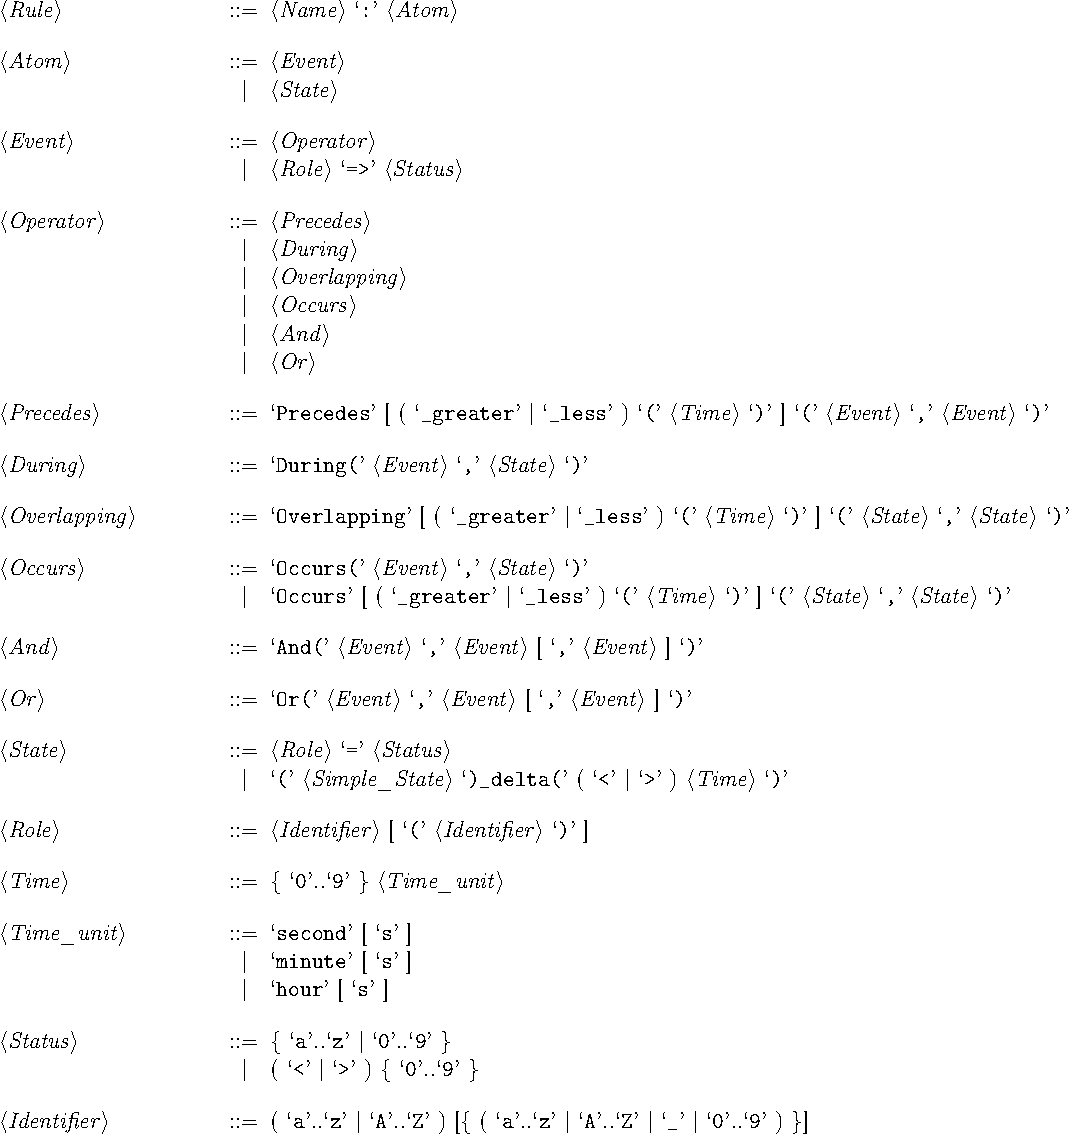
\includegraphics[scale=.8]{gfx/bnfintern.pdf}
  %\caption{bnf1.}
  \label{fig:bnf2}
\end{figure*}
\newpage
\section*{Représentation textuelle}
\begin{figure*}
  \centering
  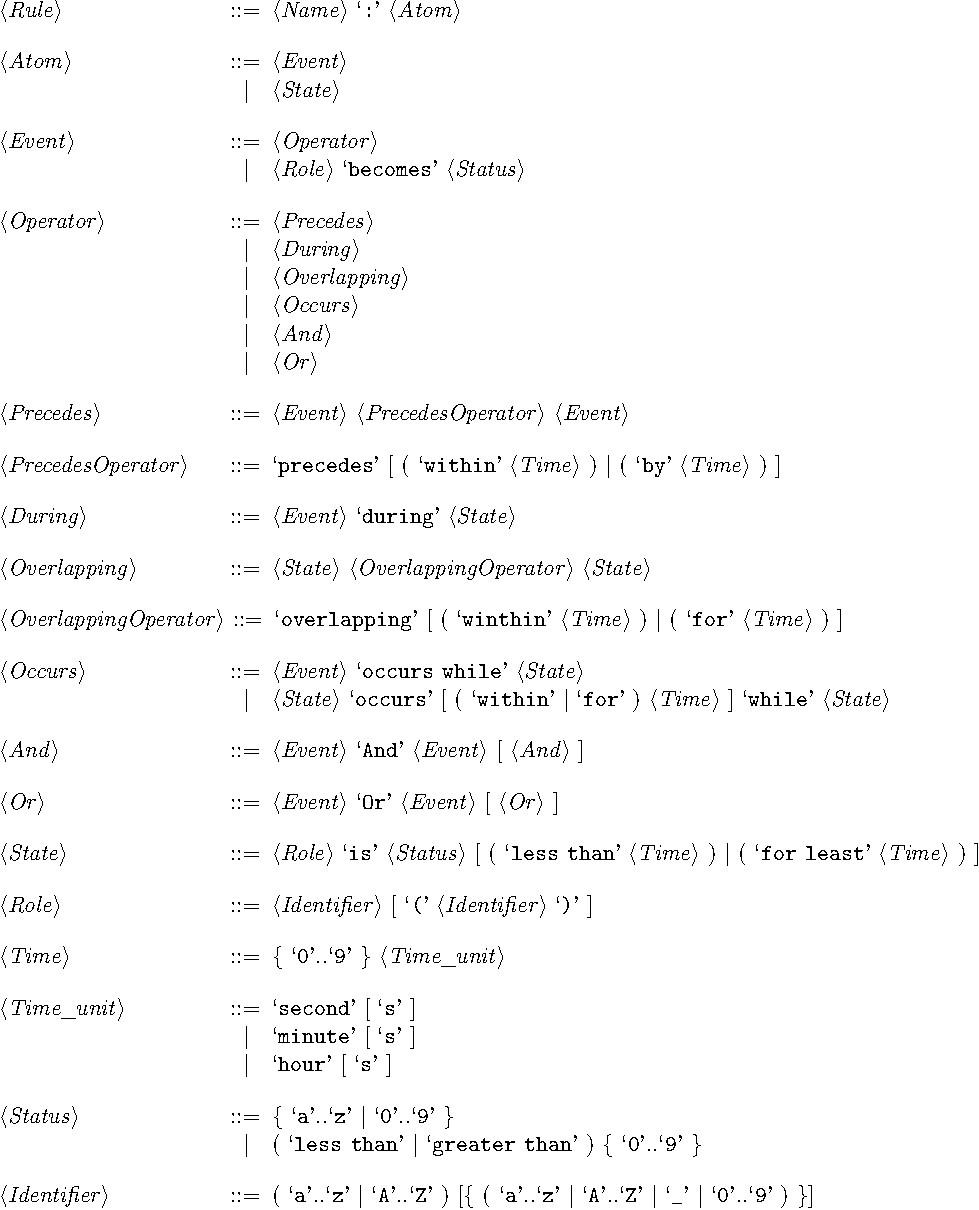
\includegraphics[scale=.8]{gfx/bnftext.pdf}
  %\caption{bnf1.}
  \label{fig:bnf1}
\end{figure*}

%\chapter{Table statique des interactions}
\begin{figure}[h!]
%\begin{footnotesize}
\begin{lstlisting}[basicstyle=\ttfamily\footnotesize]
{       
        "presence": {"kind": "Presence",
                "values": ["true", "false"]},
        "door": {"location": "Entrance","kind": "Door",
                "values": ["open", "close"]},
	"cupboard": {"location": "Kitchen", "kind": "Cupboard",
		"values": ["open", "close"]},
	"fridge": {"location": "Kitchen", "kind": "Fridge",
		"values": ["open", "close"]}, 
	"stove": {"location": "Kitchen", "kind": "Stove",
		"values": ["on", "off"]},
	"juicer": {"location": "Kitchen", "kind": "Juicer",
		"values": ["on", "off"]},
	"toaster": {"location": "Kitchen", "kind": "Toaster",
		"values": ["on", "off"]},
	"meatcleaver": {"location": "Kitchen", "kind": "Meatcleaver",
		"values": ["on", "off"]},
	"microwave": {"location": "Kitchen", "kind": "Microwave",
		"values": ["on", "off"]},
	"kettle": {"location": "Kitchen", "kind": "Kettle",
		"values": ["on", "off"]},
	"coffeeMaker": {"location": "Kitchen", "kind": "CoffeeMaker",
		"values": ["on", "off"]},
	"nightTime": {"location": "Night", "kind": "Calendar",
		"values": ["begin", "end"]},
	"dinnerTime": {"location": "Dinner", "kind": "Calendar",
		"values": ["begin", "end"]},
	"lunchTime": {"location": "Lunch", "kind": "Calendar",
		"values": ["begin", "end"]},
	"breakfastTime": {"location": "Breakfast", "kind": "Calendar",
		"values": ["begin", "end"]},
	"bedTime": {"location": "Bed", "kind": "Calendar",
		"values": ["begin", "end"]},
	"dressingTime": {"location": "Dressing", "kind": "Calendar",
		"values": ["begin", "end"]},
	"wakeUpTime": {"location": "WakeUp", "kind": "Calendar",
		"values": ["begin", "end"]}
}
\end{lstlisting}
\caption{Table statique complète des interactions dans domassist.}
\label{listing:table_static_complete}
%\end{footnotesize}
\end{figure}


%----------------------------------------------------------------------------------------
%	BIBLIOGRAPHY
%----------------------------------------------------------------------------------------
\chapter*{Bibliographie}
\label{sec:references}

\markboth{\smallcaps{Bibliographie}}{} % work-around to have small caps also

%\manualmark
%\phantomsection 
%\refstepcounter{dummy}

\addtocontents{toc}{\protect\vspace{\beforebibskip}} % to have the bib a bit from the rest in the toc
\addcontentsline{toc}{chapter}{Bibliographie}

% The entries in the bibliography are all sorted by the last name of the
% primary author.  Dashes signify that the list of authors is the same
% as the preceding bibliographic entry.

% \renewcommand{\finentrypunct}{\addperiod} % reset to dot after citations...
\printbibliography[notcategory=fullcited,heading=none]


% \bibliography{bibliography} % Use the bibliography.bib file for the bibliography
% \bibliographystyle{plainnat} % Use the plainnat style of referencing

%----------------------------------------------------------------------------------------

\printindex % Print the index at the very end of the document

\end{document}